%%
%% Copyright 2007-2025 Elsevier Ltd
%%
%% This file is part of the 'Elsarticle Bundle'.
%% ---------------------------------------------
%%
%% It may be distributed under the conditions of the LaTeX Project Public
%% License, either version 1.3 of this license or (at your option) any
%% later version.  The latest version of this license is in
%%    http://www.latex-project.org/lppl.txt
%% and version 1.3 or later is part of all distributions of LaTeX
%% version 1999/12/01 or later.
%%
%% The list of all files belonging to the 'Elsarticle Bundle' is
%% given in the file `manifest.txt'.
%%
%% Template article for Elsevier's document class `elsarticle'
%% with harvard style bibliographic references

\documentclass[preprint,12pt,authoryear]{elsarticle}

%% Use the option review to obtain double line spacing
%% \documentclass[authoryear,preprint,review,12pt]{elsarticle}

%% Use the options 1p,twocolumn; 3p; 3p,twocolumn; 5p; or 5p,twocolumn
%% for a journal layout:
%% \documentclass[final,1p,times,authoryear]{elsarticle}
%% \documentclass[final,1p,times,twocolumn,authoryear]{elsarticle}
%% \documentclass[final,3p,times,authoryear]{elsarticle}
%% \documentclass[final,3p,times,twocolumn,authoryear]{elsarticle}
%% \documentclass[final,5p,times,authoryear]{elsarticle}
%% \documentclass[final,5p,times,twocolumn,authoryear]{elsarticle}

%% For including figures, graphicx.sty has been loaded in
%% elsarticle.cls. If you prefer to use the old commands
%% please give \usepackage{epsfig}

%% The amssymb package provides various useful mathematical symbols
\usepackage{amssymb}
%% The amsmath package provides various useful equation environments.
\usepackage{amsmath}
%% The amsthm package provides extended theorem environments
%% \usepackage{amsthm}

%% The lineno packages adds line numbers. Start line numbering with
%% \begin{linenumbers}, end it with \end{linenumbers}. Or switch it on
%% for the whole article with \linenumbers.
%% \usepackage{lineno}

%% Additional packages required by the manuscript
%% (geometry, graphicx, natbib, hyperref are already loaded by elsarticle)
\usepackage{float}
\usepackage{placeins}
\usepackage{mathpazo}
\usepackage{mathtools}
\usepackage{caption}
\usepackage{subcaption}
\usepackage{colortbl}
\usepackage{longtable}
\usepackage{booktabs}
\usepackage{tikz}
\usetikzlibrary{arrows.meta,fit,backgrounds,positioning}
\usepackage{multirow}
\usepackage{enumitem}
\usepackage{tabularx}
\usepackage{array}
\usepackage[table]{xcolor}
\usepackage{pdflscape}
\usepackage{pifont}
\usepackage{mdframed}
\usepackage{rotating}
\usepackage{lscape}
\usepackage{afterpage}
\usepackage{arydshln}
\usepackage{pgfplots}
\pgfplotsset{compat=1.17}


\usepackage[normalem]{ulem}  % \sout{} for review-mode strikethrough
\usepackage[colorinlistoftodos]{todonotes}

\newcommand{\cmark}{\ding{51}} % Define command to print check mark
\newcommand{\xmark}{\ding{55}} % Define command to print x mark
% \newcommand{\dan}[1]{\textcolor{blue}{\textbf{Dan:} #1}}
% \newcommand{\ita}[1]{\textcolor{red}{\textbf{Itamar:} #1}}
% \newcommand{\itamar}[1]{\textcolor{teal}{\textbf{Itamar:} #1}}

% Define new column types for uniform styling and functionality
\newcolumntype{M}[1]{>{\centering\arraybackslash\small}m{#1}} % Small font, centered
\newcolumntype{B}[1]{>{\centering\arraybackslash\small\bfseries}m{#1}} % Bold font, centered
\newcolumntype{S}{>{\centering\arraybackslash\small\bfseries}m{0.8cm}} % Small and bold font, fixed width
\newcolumntype{T}{>{\centering\arraybackslash\tiny\bfseries}m{0.8cm}} % Small and bold font, fixed width


\newcommand{\fixme}[2]{\todo[inline,color=orange!45]{\textbf{#1:} #2}}
\newcommand{\dan}[1]{\fixme{Dan}{#1}}
\newcommand{\itamar}[1]{\fixme{Itamar}{#1}}

\journal{Applied Soft Computing Journal}

\begin{document}

\begin{frontmatter}

%% Title, authors and addresses

%% use the tnoteref command within \title for footnotes;
%% use the tnotetext command for theassociated footnote;
%% use the fnref command within \author or \affiliation for footnotes;
%% use the fntext command for theassociated footnote;
%% use the corref command within \author for corresponding author footnotes;
%% use the cortext command for theassociated footnote;
%% use the ead command for the email address,
%% and the form \ead[url] for the home page:
%% \title{Title\tnoteref{label1}}
%% \tnotetext[label1]{}
%% \author{Name\corref{cor1}\fnref{label2}}
%% \ead{email address}
%% \ead[url]{home page}
%% \fntext[label2]{}
%% \cortext[cor1]{}
%% \affiliation{organization={},
%%            addressline={},
%%            city={},
%%            postcode={},
%%            state={},
%%            country={}}
%% \fntext[label3]{}

\title{A Resource-Aware Benchmark of Feature Selection: When Does Additional Complexity Pay Off?}

%% use optional labels to link authors explicitly to addresses:
%% \author[label1,label2]{}
%% \affiliation[label1]{organization={},
%%             addressline={},
%%             city={},
%%             postcode={},
%%             state={},
%%             country={}}
%%
%% \affiliation[label2]{organization={},
%%             addressline={},
%%             city={},
%%             postcode={},
%%             state={},
%%             country={}}

\author{} %% Author name

%% Author affiliation
% \affiliation{organization={},%Department and Organization
%             addressline={},
%             city={},
%             postcode={},
%             state={},
%             country={}}

%% Abstract
\begin{abstract}
Feature selection (FS) practitioners face fragmented guidance when choosing among dozens of algorithms with substantially different resource requirements. We present a resource-oriented FS benchmark spanning five practical dimensions---runtime, method family, supervision, implementation effort, and optimization effort---covering 37 algorithms across 102 datasets. Rather than ranking individual algorithms, we group methods by resource cost and conduct paired within-dataset comparisons to test whether higher-cost categories consistently outperform lower-cost alternatives. Using Wilcoxon signed-rank tests, win rates, and Cliff's delta, we find that higher-cost resources typically provide no systematic performance advantage: fast methods match or outperform slow ones, library implementations match or exceed research-code methods, and simple Filter methods match or exceed complex alternatives. Supervision is the main exception, yielding consistent gains, although this advantage weakens on harder datasets. The largest effect is optimization: untuned FS degrades performance by 7--12 AUC points below the no-FS baseline, while proper tuning within low-cost categories recovers this baseline. Notably, the no-FS baseline itself frequently matches or exceeds FS methods, suggesting that FS should often be valued for dimensionality reduction, interpretability, or efficiency rather than predictive gains alone. These findings support a practical default: in most settings, practitioners should begin with fast, library-based, simple methods and tune them systematically before escalating to more expensive alternatives. 
\end{abstract}

\begin{graphicalabstract}
    \hspace*{-0.15\linewidth}
    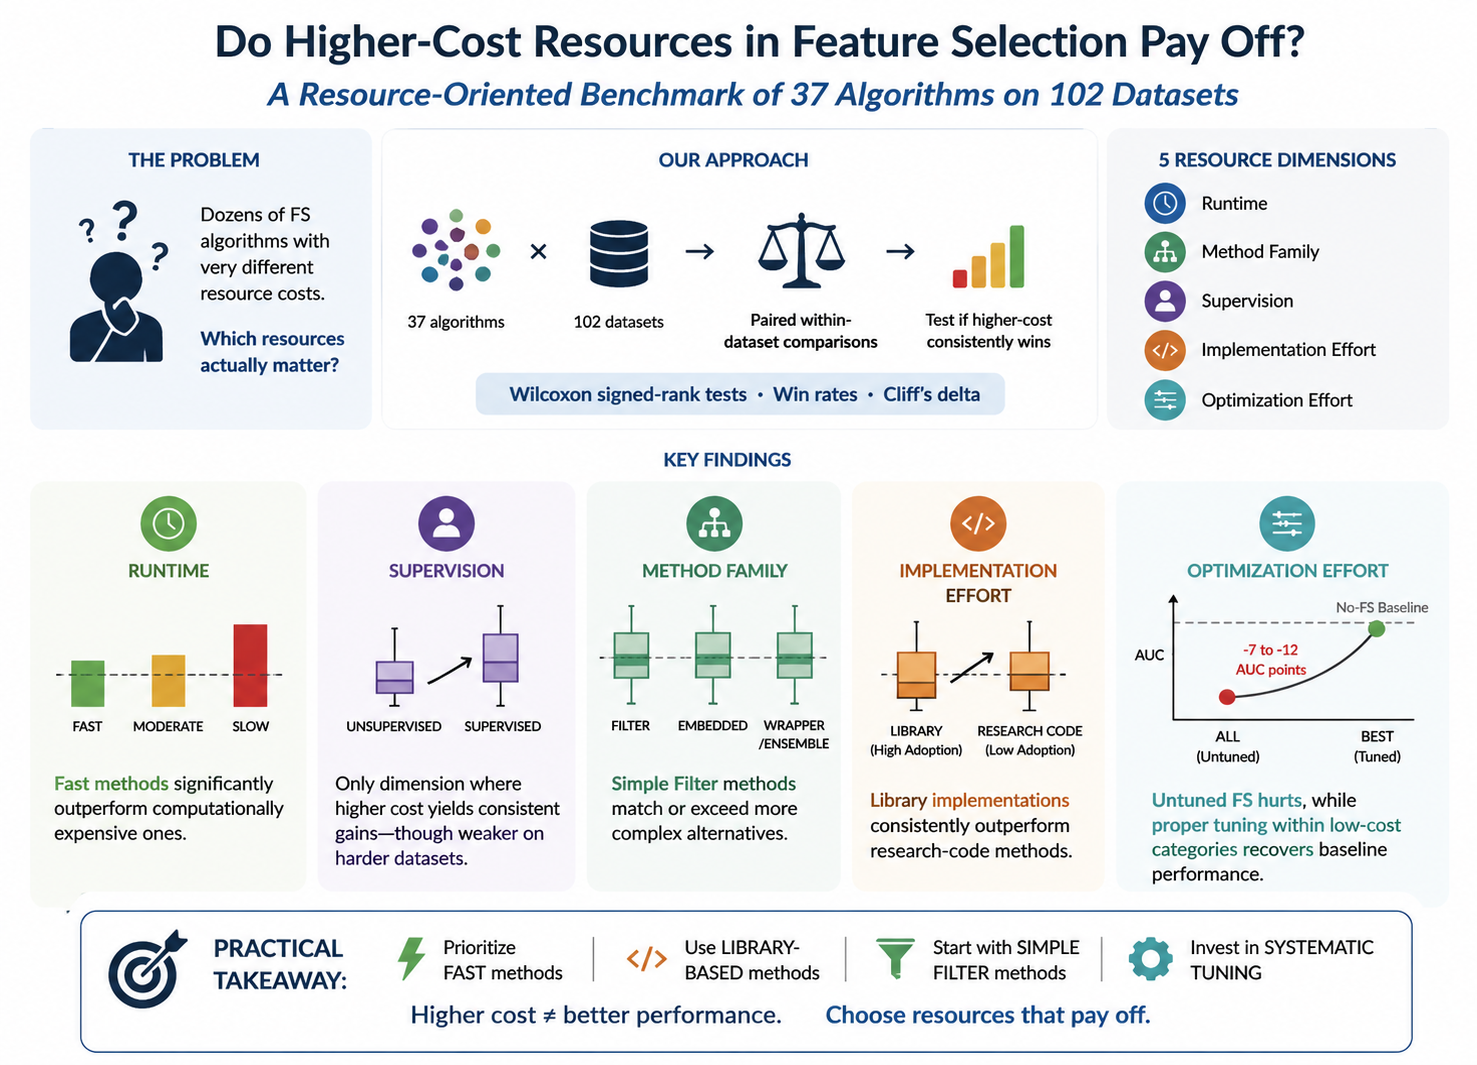
\includegraphics[width=1.3\linewidth]{assets/graphical_abstract.png}
\end{graphicalabstract}

\begin{highlights}
\item First resource-aware FS benchmark: 37 algorithms, 102 datasets, 5 cost dimensions
\item Higher resource cost provides no systematic predictive advantage in most dimensions
\item Fast, library-based, simple methods match or outperform complex alternatives
\item Untuned FS degrades performance by 7--12 AUC points below the no-FS baseline
\item Conclusions backed by paired Wilcoxon tests, win rates, and Cliff's delta at scale
\end{highlights}
\begin{keyword}
Feature selection \sep Benchmarking \sep Resource-aware learning \sep Computational cost \sep Implementation effort \sep Method comparison \sep Practical machine learning
\end{keyword}

% %% Keywords
% \begin{keyword}
% %% keywords here, in the form: keyword \sep keyword

% %% PACS codes here, in the form: \PACS code \sep code

% %% MSC codes here, in the form: \MSC code \sep code
% %% or \MSC[2008] code \sep code (2000 is the default)

% \end{keyword}

\end{frontmatter}

%% Add \usepackage{lineno} before \begin{document} and uncomment
%% following line to enable line numbers
%% \linenumbers

%% main text

\section{Introduction}
\label{chapter:intro}

High-dimensional data are common in bioinformatics, genomics, image processing, text mining, and other applied domains. In such settings, feature selection (FS) is often introduced as a way to reduce dimensionality, remove irrelevant or redundant variables, improve interpretability, and sometimes improve predictive performance \citep{bellman1957dynamic,donoho2000high,guyon2003introduction}. Yet the practical value of FS remains difficult to assess. Although the motivation is clear, the effect of FS depends on the dataset, the downstream learner, the number of selected features, and the amount of tuning invested. A basic question is therefore often left unresolved: does FS improve prediction relative to using all features, or is its value mainly computational and interpretive?

A practical issue that is often underemphasized is that FS itself consumes resources. A simple variance filter is transparent, requires little or no tuning, and runs quickly. In contrast, wrapper, neural, or metaheuristic-based methods may require substantial runtime, careful hyperparameter tuning, and non-trivial implementation effort. Thus, the relevant question is not only whether FS can improve performance, but whether the improvement justifies the resources required to obtain it. This question is especially important because several empirical studies suggest that strong learners and simple FS methods often perform competitively, while complex FS procedures may yield limited gains or even degrade performance due to instability or overfitting \citep{eklund2014choosing,nguyen2015unbiased,bommert2020benchmark,Grinsztajn22,zschaubitz2025benchmark}.

The abundance of FS algorithms reflects the absence of a universal best method. Numerous surveys classify FS methods by family, supervision, or data type, and compare their performance across collections of datasets \citep{weston2000feature,chandrashekar2014survey,bolon2014review,li2017feature,bommert2020benchmark,bommert2022benchmark,jiao2023survey}. Meta-learning approaches go further by learning per-dataset recommendations from meta-features \citep{filchenkov2015datasets,PARMEZAN20171}. These approaches are useful when the goal is to recommend a concrete algorithm for a concrete dataset, but they do not directly answer a simpler preceding question: before invoking a recommender or implementing a costly method, is escalation beyond low-cost FS justified at all in terms of predictive performance?

This paper addresses that question through a resource-aware empirical benchmark. Instead of ranking individual algorithms, we group 37 FS methods by practical resource dimensions---runtime, method family, supervision, implementation effort, and optimization effort---and test whether higher-cost categories consistently outperform lower-cost alternatives across 102 datasets. We further combine this resource view with dataset-hardness regimes and paired within-dataset dominance tests, allowing us to ask not only which methods perform well, but whether additional resource investment systematically pays off. This also explicitly tests the no-FS baseline, asking when FS improves prediction and when using all features is already competitive.

This framing connects to standard applied machine-learning advice: start with simple methods, tune carefully, and only then add complexity \citep{kuhn2013applied,kuhn2019feature,geron2019hands,domingos2012few}. Our contribution is to operationalize this principle specifically for FS at scale. We quantify whether slower methods, research-code implementations (i.e., methods implemented from papers rather than standard libraries), more complex families, and supervised selectors dominate cheaper alternatives, and whether the answer changes with dataset difficulty. In this sense, our framework is complementary to per-dataset meta-learning: it provides a transparent first decision layer. If tuned low-cost methods are sufficient, practitioners can avoid unnecessary complexity; if they fail, there is a clearer rationale for escalating to meta-learning or broader algorithm search.

Table~\ref{tab:survey_papers} summarizes representative prior benchmarking and recommendation studies, highlighting the comparatively limited scale or resource coverage of most previous evaluations.


\begin{figure*}[t]
\centering
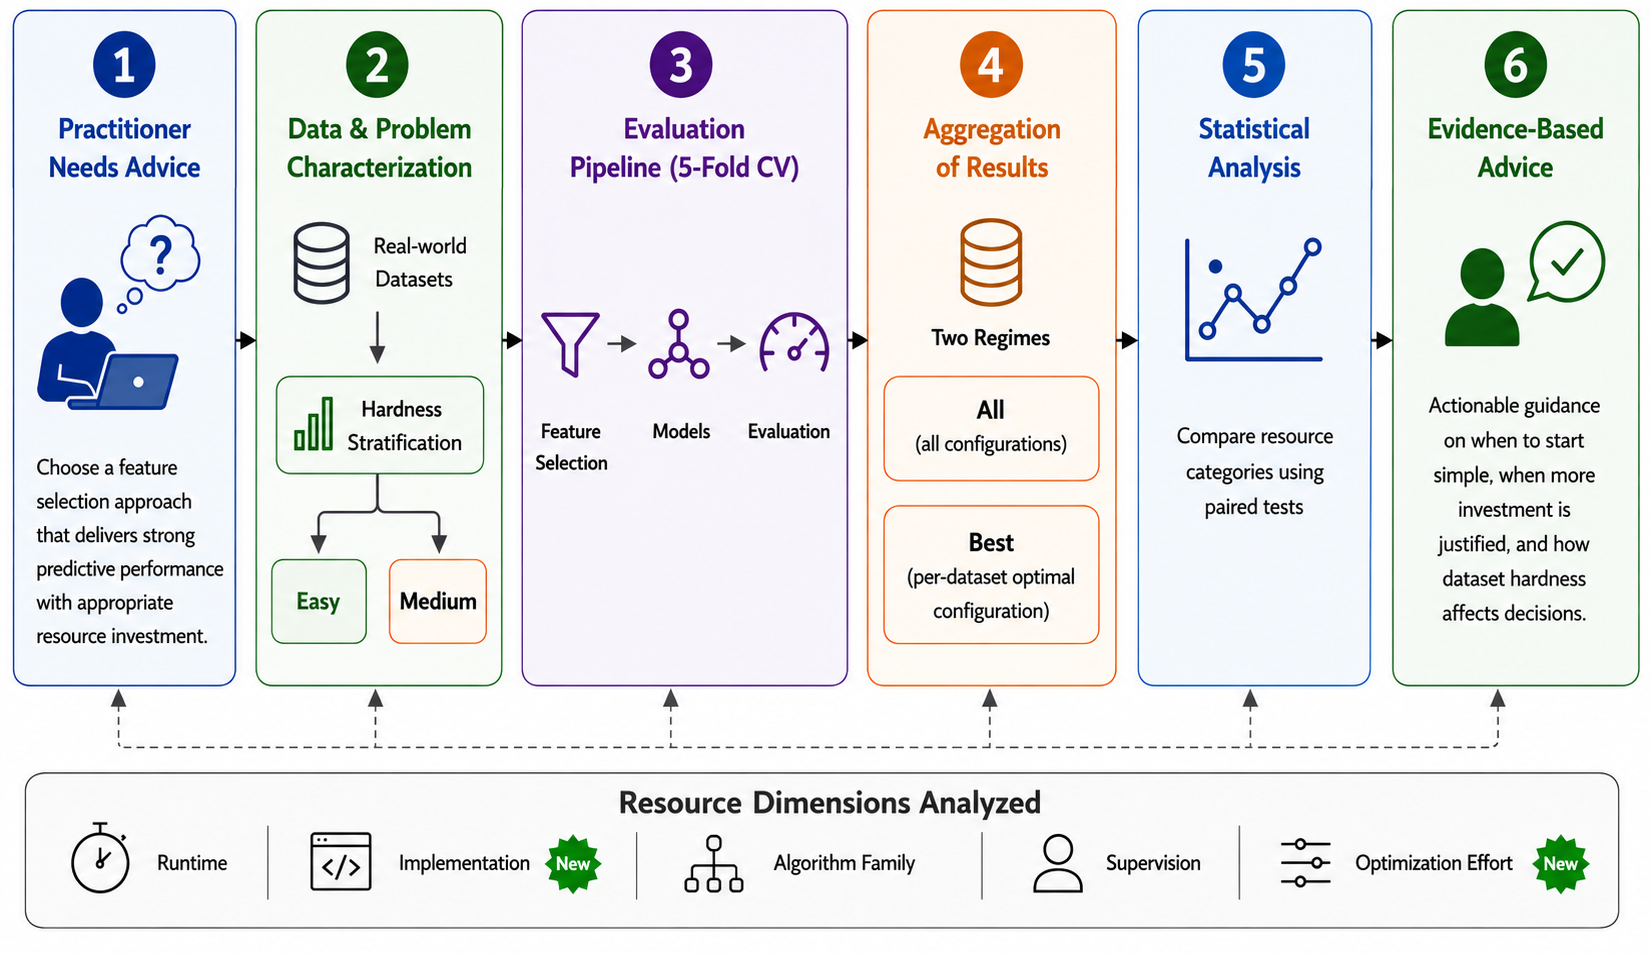
\includegraphics[width=\textwidth]{assets/pipeline_intro_genera.png}
\caption{High-level overview of the proposed resource-aware feature-selection framework. The framework starts from a practitioner seeking guidance under practical resource constraints, and proceeds through dataset characterization, large-scale benchmarking, cross-validated evaluation, aggregation across optimization regimes, and paired statistical analysis. The resulting evidence is translated into actionable guidance regarding when low-cost feature-selection methods are sufficient and when additional resource investment may be justified.}
\label{fig:framework_overview}
\end{figure*}


\begin{table}[h!]
\centering 
\caption{Summary statistics for prominent feature-selection benchmarking, survey, and algorithm-selection studies. Papers are sorted approximately by number of citations. The table shows the typically limited number of datasets and algorithms considered in prior work.}
\label{tab:survey_papers}
{\small
\begin{tabularx}{\textwidth}{|>{\centering\arraybackslash}X|>{\centering\arraybackslash}X|>{\centering\arraybackslash}X|>{\centering\arraybackslash}X|}
\hline
\textbf{Paper} & \textbf{\#Citations} & \textbf{\# Datasets} & \textbf{\# Algorithms} \\
\hline
\citep{chandrashekar2014survey} & 5728 & 7 & 2 \\
\hline
\citep{bolon2014review} & 756 & 9 & 7 \\
\hline
\citep{filchenkov2015datasets} & 55 & 84 & 16 \\
\hline
\citep{li2017feature} & 3353 & 29 & 34 \\
\hline
\citep{PARMEZAN20171} & 77 & 150 & 4 \\
\hline
\citep{zhang2019unsupervised} & 126 & 16 & 8 \\
\hline
\citep{bommert2020benchmark} & 636 & 16 & 22 \\
\hline
\citep{bommert2022benchmark} & 107 & 14 & 11 \\
\hline
\citep{tanveer2022large} & 38 & 14 & 11 \\
\hline
\citep{jiao2023survey} & 57 & 2 & 23 \\
\hline
\end{tabularx}

\vspace{2mm}
\raggedright

}
\end{table}


\paragraph{Contributions and empirical takeaways}
This paper makes four main contributions, illustrated schematically in Figure~\ref{fig:framework_overview}. First, we conduct a large-scale empirical study of 37 FS algorithms across 102 real-world datasets (Table~\ref{tab:all_datasets}), including both binary and multiclass settings. Second, to the best of our knowledge, this is the first comprehensive resource-oriented FS benchmark that explicitly defines, measures, and compares practical resource axes (Table~\ref{tab:fs_resource_summary}). Rather than ranking individual algorithms, we group methods by runtime, implementation effort, method family, supervision, and optimization effort, and ask whether moving to a higher-cost category is empirically justified. Third, we introduce implementation effort as a practical resource: methods available through standard libraries are distinguished from methods that require research-level implementation, adaptation, or validation. This dimension captures a real cost faced by practitioners but is rarely treated as an explicit axis in FS benchmarking. Fourth, we combine this resource view with the dataset-hardness taxonomy of \citep{elmakias2025choosing} (Table~\ref{tab:auc_performance_all}), allowing us to ask whether resource investment behaves differently on Easy and Medium datasets rather than only on average across all problems (see Section~\ref{sec:related} for details on the Easy--Medium taxonomy). This provides a low-dimensional alternative to richer descriptions of dataset complexity, such as those produced by the Problexity library \citep{Komorniczak2023Problexity}. While such descriptors are informative, they can also lead to highly nuanced, dataset-specific analyses that are difficult to translate into simple resource-level guidance, as reflected in the meta-learning setting of \citep{PARMEZAN20171}.

\begin{table}[t]
\centering
\footnotesize
\caption{Distribution of the 37 feature selection algorithms across resource dimensions. Each row corresponds to a resource, and columns (C1--C5) denote its categories.}
\label{tab:fs_resource_summary}

\resizebox{\linewidth}{!}{
\begin{tabular}{lccccc}
\toprule
\textbf{Resource} & \textbf{C1} & \textbf{C2} & \textbf{C3} & \textbf{C4} & \textbf{C5} \\
\midrule
Runtime
& 20 (Fast)
& 6 (Moderate)
& 4 (Slow)
& 7 (Mixed)
& -- \\

Implementation
& 11 (Library)
& 26 (Article)
& --
& --
& -- \\

Supervision
& 29 (Supervised)
& 8 (Unsupervised)
& --
& --
& -- \\

Family
& 11 (Filter)
& 6 (Wrapper)
& 13 (Embedded)
& 3 (Ensemble)
& 4 (Hybrid) \\

\bottomrule
\end{tabular}
}
\end{table}

A central contribution of the framework is the distinction between two optimization regimes. The \emph{All} setting represents a low-effort scenario: all configurations are pooled across algorithms, values of $K$ (the number of selected features), and hyperparameters of the FS algorithm, reflecting what may happen when a practitioner applies FS without systematic tuning. The \emph{Best} setting represents a higher-effort scenario: for each dataset and resource category, we retain the configuration that achieves the highest performance, approximating a practitioner who searches over several algorithms, values of $K$, and recommended parameter settings under a fixed resource budget. This distinction allows us to separate the effect of FS itself from the effect of optimization effort.

The largest empirical effect we observe is precisely this optimization effect. In the \emph{All} setting, applying FS without systematic tuning substantially degrades performance relative to the no-FS baseline, by approximately $7$ AUC points on Easy datasets and $12$ AUC points on Medium datasets. In contrast, in the \emph{Best} setting, performance typically recovers to the no-FS level in at least one low-cost category of each resource. This suggests that, when practitioners allocate effort to FS, the first investment should be in trying several low-cost methods, several values of $K$, and reasonable configurations, before escalating to slower, harder-to-implement, or more complex methods. Full details of the optimization framework are given in Section~\ref{sec:resource_dimensions}.

Our statistical analysis uses paired within-dataset comparisons to assess whether higher-cost categories consistently outperform lower-cost alternatives. For each dataset, we compare the best-performing configuration in a higher-cost category with the corresponding best-performing configuration in the lower-cost category, using one-sided Wilcoxon signed-rank tests complemented by win rates and Cliff's delta effect sizes. This approach controls for dataset-level heterogeneity and provides a direct test of whether additional resource investment yields consistent gains.

The results reveal a consistent pattern: in most resource dimensions, higher-cost categories do not systematically dominate lower-cost ones. For runtime, slow methods are significantly dominated by fast methods (Cliff's $\delta = 0.72$ for Easy datasets), indicating that additional runtime investment often fails to improve performance and may even degrade it. For implementation effort, library methods consistently match or exceed research-code implementations (Cliff's $\delta = 0.36$ for Easy, $0.64$ for Medium), an effect that grows with dataset difficulty and suggests that research-code methods may be more sensitive to suboptimal conditions or harder-to-tune settings. For method families, simple Filter methods match or exceed more complex alternatives, with Hybrid methods being significantly dominated. Only supervision shows the expected pattern where higher cost provides advantages, and this effect weakens substantially for Medium datasets.

Under this evidence, the practical implication is not that a single simple method is universally best, but rather that low-cost, transparent methods constitute a strong default starting point. More expensive FS machinery should be introduced only when systematic low-cost search fails to provide satisfactory performance.

\paragraph{From resource categories to algorithm-level guidance}
A natural concern is that ``low cost'' along one resource axis may not imply low cost along others: for example, an algorithm may be fast but difficult to implement, or library-based but sensitive to tuning. To operationalize the resource-level analysis, Table~\ref{tab:meta_resource} summarizes the algorithms by their combined cost profiles across runtime, tuning, and implementation effort. The table shows that low-resource behavior is not merely an artifact of a single dimension; rather, a subset of methods consistently exhibits favorable properties across multiple resources, including fast runtime, limited tuning requirements, and stable implementations. This allows us to translate the resource-level findings into practical starting points, while still avoiding the stronger claim that any single algorithm is universally best.

\vspace{1mm}

The remainder of the paper is organized as follows. Section~\ref{sec:related} reviews the relevant literature. Section~\ref{sec:method} describes the proposed methodology and statistical framework. Section~\ref{sec:results} presents the empirical results. Finally, Section~\ref{sec:discussion} discusses implications, limitations, and future directions.

\begin{table}[t]
\centering
\caption{Meta-resource categorization of all feature selection algorithms based on combined cost across runtime, tuning, and implementation effort. Supervision is not used as a defining axis; instead, each algorithm is annotated with (S) for supervised and (U) for unsupervised. Complete description of algorithms is given in Table~\ref{tab:FS_algs}. HSIC Lasso and ReliefF have tunable parameters, but are included in the Simple category based on their observed runtime and implementation accessibility relative to the other methods in the benchmark.}
\resizebox{\textwidth}{!}{
\begin{tabular}{|l|p{4cm}|p{4cm}|p{7cm}|}
\hline
\textbf{Category} & \textbf{Characteristics} & \textbf{Typical Properties} & \textbf{Algorithms} \\
\hline

\textbf{Simple}
& Consistently low cost across resources; readily usable in practice
& Fast runtime, minimal or no hyperparameters, stable standard library implementations, easy to deploy and interpret
& Low Var (U), UnivariateFS (S), ETree (S), AdaBoost (S), SVC (S), Skewness (U), ReliefF (S), Fisher Score (S), HSIC Lasso (S) \\
\hline

\textbf{Mixed}
& Low cost in some dimensions, higher in others
& Moderate runtime or tuning requirements
& mRMR (S), SHAP (S), RFS (S), MCFS (U), CAE (U), DLFS (S), UFS (U), STG (S), LSPIN (S), RFE (S), Stability-LASSO (S), Boruta (S) \\
\hline

\textbf{Complex}
& High cost across multiple resources
& Long runtime ($\geq$1 hr), extensive tuning, research-level or custom implementations, higher engineering and interpretation effort
& DecisionT\_B (S), DecisionT\_F (S), SVM\_B (S), SVM\_F (S), LeadingEV (S), Alpha Inv (S), LS (U), CT (U), DT (U), SVM RBF (S), GRAPH (S), GRACES (S), CEI-GA (S), SA-FS (S), Filter-Wrapper (S), PSO-FS (S) \\
\hline

\end{tabular}
}

\label{tab:meta_resource}
\end{table}


{\small
\begin{table}[t!]
\centering
\caption{Summary of the 37 feature selection algorithms evaluated in this study, annotated by method family, supervision, hyperparameter requirements, typical runtime, and implementation source. Method families are denoted as follows: F = Filter, W = Wrapper, E = Embedded, En = Ensemble-embedded, H = Hybrid. Typical runtime categories are: Fast ($<1$\,min), Moderate (1\,min--1\,hr), Slow ($>1$\,hr), and Mixed (no dominant runtime category across runs). Since runtime varies across datasets, these categories are defined by aggregating each algorithm’s executions across all datasets, as detailed in Section~\ref{sec:method}, and selecting the dominant bucket.}
\resizebox{\textwidth}{!}{%
\begin{tabular}{|c|l|c|c|c|c|c|}
\hline
\textbf{\#}
  & \textbf{Algorithm}
  & \textbf{Family}
  & \textbf{Supervised}
  & \textbf{Hyperparams}
  & \textbf{Typical Runtime}
  & \textbf{Implementation} \\
\hline
1  & SA-FS \cite{kirkpatrick1983optimization}   & H  & \checkmark & \checkmark & Fast     & Article \\
2  & ReliefF \cite{kira1992feature}            & F  & \checkmark & \checkmark & Fast     & Article \\
3  & DecisionT\_B \cite{guyon2003introduction} & W  & \checkmark & \checkmark & Slow     & Article \\
4  & DecisionT\_F \cite{guyon2003introduction} & W  & \checkmark & \checkmark & Mixed    & Article \\
5  & SVM\_B \cite{guyon2003introduction}       & W  & \checkmark & \checkmark & Slow     & Article \\
6  & SVM\_F \cite{guyon2003introduction}       & W  & \checkmark & \checkmark & Mixed    & Article \\
7  & RFE \cite{guyon2003introduction}          & W  & \checkmark & \checkmark & Fast     & Library \\
8  & Filter-Wrapper \cite{guyon2003introduction} & H & \checkmark & \checkmark & Fast    & Article \\
9  & LeadingEV \cite{d2004direct}              & F  & \checkmark & \checkmark & Moderate & Article \\
10 & LS \cite{he2005laplacian}                 & F  & \xmark     & \checkmark & Fast     & Article \\
11 & Alpha Inv \cite{zhou2005streaming}        & W  & \checkmark & \checkmark & Fast     & Article \\
12 & mRMR \cite{peng2005feature}               & F  & \checkmark & \checkmark & Mixed    & Library \\
13 & ETree \cite{geurts2006extremely}          & En & \checkmark & \checkmark & Fast     & Library \\
14 & CT \cite{Bickel2008CovarianceMatrices}    & F  & \xmark     & \xmark     & Moderate & Article \\
15 & AdaBoost \cite{hastie2009multi}           & En & \checkmark & \checkmark & Fast     & Library \\
16 & DT \cite{johnstone2009consistency}        & F  & \xmark     & \xmark     & Fast     & Article \\
17 & MCFS \cite{cai2010unsupervised}           & E  & \xmark     & \xmark     & Fast     & Article \\
18 & RFS \cite{nie2010efficient}               & E  & \checkmark & \checkmark & Moderate & Article \\
19 & Stability-LASSO \cite{meinshausen2010stability} & E & \checkmark & \checkmark & Fast & Article \\
20 & Boruta \cite{kursa2010boruta}             & En & \checkmark & \checkmark & Mixed    & Library \\
21 & SVM RBF \cite{liu2011feature}             & E  & \checkmark & \checkmark & Slow     & Library \\
22 & Low Var \cite{pedregosa2011scikit}        & F  & \xmark     & \xmark     & Fast     & Library \\
23 & UnivariateFS \cite{pedregosa2011scikit}   & F  & \checkmark & \checkmark & Fast     & Library \\
24 & Fisher Score \cite{gu2012generalized}     & F  & \checkmark & \xmark     & Fast     & Article \\
25 & GRAPH \cite{ye2012sparse}                 & E  & \checkmark & \checkmark & Slow     & Article \\
26 & PSO-FS \cite{xue2012particle}             & H  & \checkmark & \checkmark & Fast     & Article \\
27 & HSIC Lasso \cite{yamada2014high}          & F  & \checkmark & \checkmark & Fast     & Library \\
28 & SVC \cite{abraham2014machine}             & E  & \checkmark & \checkmark & Fast     & Library \\
29 & SHAP \cite{lundberg2017unified}           & E  & \checkmark & \checkmark & Mixed    & Library \\
30 & CAE \cite{balin2019concrete}              & E  & \xmark     & \checkmark & Moderate & Article \\
31 & STG \cite{yamada2020feature}              & E  & \checkmark & \checkmark & Fast     & Article \\
32 & DLFS \cite{wojtas2020feature}             & E  & \checkmark & \checkmark & Moderate & Article \\
33 & UFS \cite{cheng2021algorithmic}           & E  & \xmark     & \checkmark & Moderate & Article \\
34 & LSPIN \cite{yang2022locally}              & E  & \checkmark & \checkmark & Fast     & Article \\
35 & GRACES \cite{chen2023graph}               & E  & \checkmark & \checkmark & Mixed    & Article \\
36 & Skewness \cite{hochma2024efficient}       & F  & \xmark     & \xmark     & Fast     & Article \\
37 & CEI-GA \cite{nematzadeh2024feature}       & H  & \checkmark & \checkmark & Mixed    & Article \\
\hline
\end{tabular}}
\vspace{1mm}
\label{tab:FS_algs}
\end{table}




\section{Related Work}\label{sec:related}

Four strands of prior work motivate the present study. First, feature-selection (FS) surveys and benchmarks have established the standard algorithmic taxonomies but often compare limited sets of algorithms and datasets. Second, meta-learning approaches attempt to recommend FS methods from dataset characteristics. Third, recent resource-aware benchmarks emphasize runtime and tuning cost, but usually do not treat implementation effort, supervision, and optimization effort as explicit resource dimensions. Fourth, dataset-hardness frameworks provide a way to ask whether conclusions about FS change as problem difficulty increases.

\paragraph{Feature-selection surveys and benchmark practice}
FS methods are commonly organized into filter, wrapper, embedded, ensemble, and hybrid families \citep{Saeys2007Review}. This taxonomy remains useful because it captures broad differences in how methods operate: filters score features independently of the downstream learner, wrappers repeatedly evaluate feature subsets through model training, embedded methods select features as part of model fitting, ensembles aggregate multiple selectors, and hybrids combine several stages. Numerous surveys have mapped this landscape and its applications, particularly in high-dimensional domains such as bioinformatics and text mining \citep{weston2000feature,guyon2003introduction,chandrashekar2014survey,bolon2014review,li2017feature,bommert2020benchmark,bommert2022benchmark,jiao2023survey}. However, many empirical comparisons remain limited in the number of datasets, algorithms, or practical costs considered. As a result, they often identify dataset-specific winners without yielding clear guidance about when additional FS complexity is worth its cost.

\paragraph{Meta-learning and algorithm recommendation}
Recommending an FS method for a given dataset is a special case of automated algorithm selection \citep{kerschke2019automated}. Early FS-specific meta-learning work argued that FS requires preprocessing-specific meta-features rather than simply reusing classifier-oriented descriptors \citep{filchenkov2015datasets}. Subsequent studies modeled FS recommendation as a supervised meta-learning task, showing that dataset meta-features can carry useful signal for predicting strong FS choices \citep{PARMEZAN20171,auto_recommend_fs_2021}. Related work further shows that meta-feature engineering itself matters: many meta-features are redundant or non-informative, and compact meta-representations can sometimes preserve recommendation quality while reducing runtime \citep{meta_feature_selection_arxiv2021,explain_meta_features_2023}. These approaches are valuable because they provide per-dataset recommendations. Our goal is complementary: rather than asking which specific FS algorithm should be recommended for a particular dataset, we ask a more resource-level question---whether moving from low-cost to higher-cost FS categories is empirically justified in the first place.

\paragraph{Resource-aware benchmarking}
Runtime was historically treated as a secondary descriptive statistic in FS benchmarks, but recent studies have begun to treat it as a primary objective. The closest line of work is by Bommert and colleagues. \citet{Bommert2019FilterBenchmark} benchmarked 22 filter methods across 16 high-dimensional datasets and explicitly studied the trade-off between predictive performance and runtime, showing that no single filter dominates across all datasets. A follow-up study on high-dimensional survival data recommended the simple variance filter over more complex alternatives partly because of its low tuning burden \citep{Bommert2022FilterFSurvival}. These studies establish that computational cost and tuning effort matter, but their scope is narrower than ours: they focus mainly on filter methods and hardware execution costs. In contrast, we treat FS as a broader resource-allocation problem that includes runtime, implementation effort, supervision, method family, and optimization effort.

\paragraph{Dataset hardness and complexity}
A separate line of work asks how to characterize the difficulty of a dataset itself. General dataset-complexity measures describe properties such as overlap, separability, dimensionality, class imbalance, neighborhood structure, and linearity, and are implemented in tools such as the Problexity library \citep{Komorniczak2023Problexity}. These measures are informative, but their high-dimensional nature can make it difficult to translate them into simple benchmarking or resource-allocation rules.

The dataset-hardness taxonomy of \citet{elmakias2025choosing} provides a lower-dimensional alternative tailored to FS benchmarking. Their framework categorizes binary datasets using the performance of a learning pipeline with and without FS. AUC values are first grouped into three performance tiers: High ($\mathrm{AUC}\geq 0.90$), Fair ($0.70 \leq \mathrm{AUC}<0.90$), and Low ($\mathrm{AUC}<0.70$). Datasets are then labeled \emph{Easy} when the best FS pipeline reaches the High tier, \emph{Medium} when performance remains in the Fair tier, and \emph{Hard} when both the no-FS and FS pipelines remain in the Low tier. A separate \emph{Fragile} category is defined for cases where applying FS degrades performance enough to move the dataset to a lower performance tier. However, under the updated AUC-based categorization used in this study, no real-world dataset falls into the Fragile category; the main AUC-based resource analysis therefore focuses on the Easy and Medium regimes.

A key empirical finding of \citet{elmakias2025choosing}, which is also reflected in the updated AUC-based categorization used here, is that genuinely Hard real-world FS benchmarks are rare. Among the 63 binary real-world datasets considered in this study, none are labeled Hard or Fragile; 48 are categorized as Easy and 15 as Medium. Two Hard datasets were obtained only through a synthetic peeling procedure in the original hardness study. This scarcity is central to our study. Since the Hard regime is not sufficiently populated by real-world datasets for reliable resource-level inference, we focus our analysis on the Easy and Medium regimes. This allows us to ask whether FS's cost-benefit behavior changes as difficulty increases, while avoiding unsupported conclusions about a Hard regime for which there is too little real-world evidence.

\paragraph{Simple baselines and the scale-of-benchmarks critique}
Finally, several empirical studies show that complex methods do not reliably dominate simpler, well-tuned baselines. \citet{haury2011influence} found that a plain $t$-test matched or outperformed SVM-RFE and greedy wrappers on gene-expression data in both accuracy and stability, while \citet{eklund2014choosing} reported no statistically significant improvement from FS when the downstream learner was a random forest. \citet{BolonCanedo2014ReviewMicroarrayFS} also showed that statistically significant differences between FS algorithms are difficult to establish on small-$N$ microarray benchmarks. This literature does not imply that simple methods are always better, but it motivates a conservative empirical question: before adopting more complex FS procedures, is there evidence that the additional resource investment systematically pays off?

Together, these strands motivate our resource-aware design. Meta-learning studies provide per-dataset recommendations, but require additional meta-feature machinery and do not directly answer whether added resource investment is worthwhile. Existing resource-aware benchmarks show that runtime matters, but do not jointly analyze runtime, implementation effort, supervision, method family, and optimization effort. Dataset-hardness work shows that most standard benchmarks are Easy and that real-world Hard datasets are scarce. Our study combines these perspectives by evaluating FS as a resource-allocation problem across explicit cost dimensions and across Easy and Medium dataset regimes.

\section{Methodology}\label{sec:method}

Our goal is to evaluate FS algorithms through a unified, large-scale pipeline that measures their cost--benefit behavior across multiple \emph{resource dimensions}. Concretely, we evaluate each FS algorithm across datasets and record its behavior along five dimensions: (i) runtime, (ii) methodological complexity (algorithm family), (iii) supervision (label usage), (iv) implementation effort, and (v) optimization effort. Predictive performance serves as the primary outcome used to compare these resource categories.

Orthogonally to these dimensions, we stratify the binary analysis according to the dataset-hardness taxonomy of \cite{elmakias2025choosing}, where datasets are categorized based on the no-FS baseline AUC and the utility of FS in improving performance. This taxonomy partitions datasets into Easy, Medium, and Hard regimes. We analyze Easy and Medium datasets only; the Hard regime contains too few datasets for reliable resource-level inference. Thus, beyond comparing categories within each resource dimension, we also examine whether the conclusions are sensitive to dataset difficulty.

Figure~\ref{fig:fs_pipeline} provides a schematic overview of the complete evaluation pipeline, which we describe in detail below.
% %% Feature-Selection Evaluation Pipeline — TikZ figure
%% Requires in preamble (after \usepackage{tikz}):
%%   \usetikzlibrary{arrows.meta,fit,backgrounds,positioning}

\begin{figure}[tbp]
\centering
\resizebox{0.98\linewidth}{!}{%
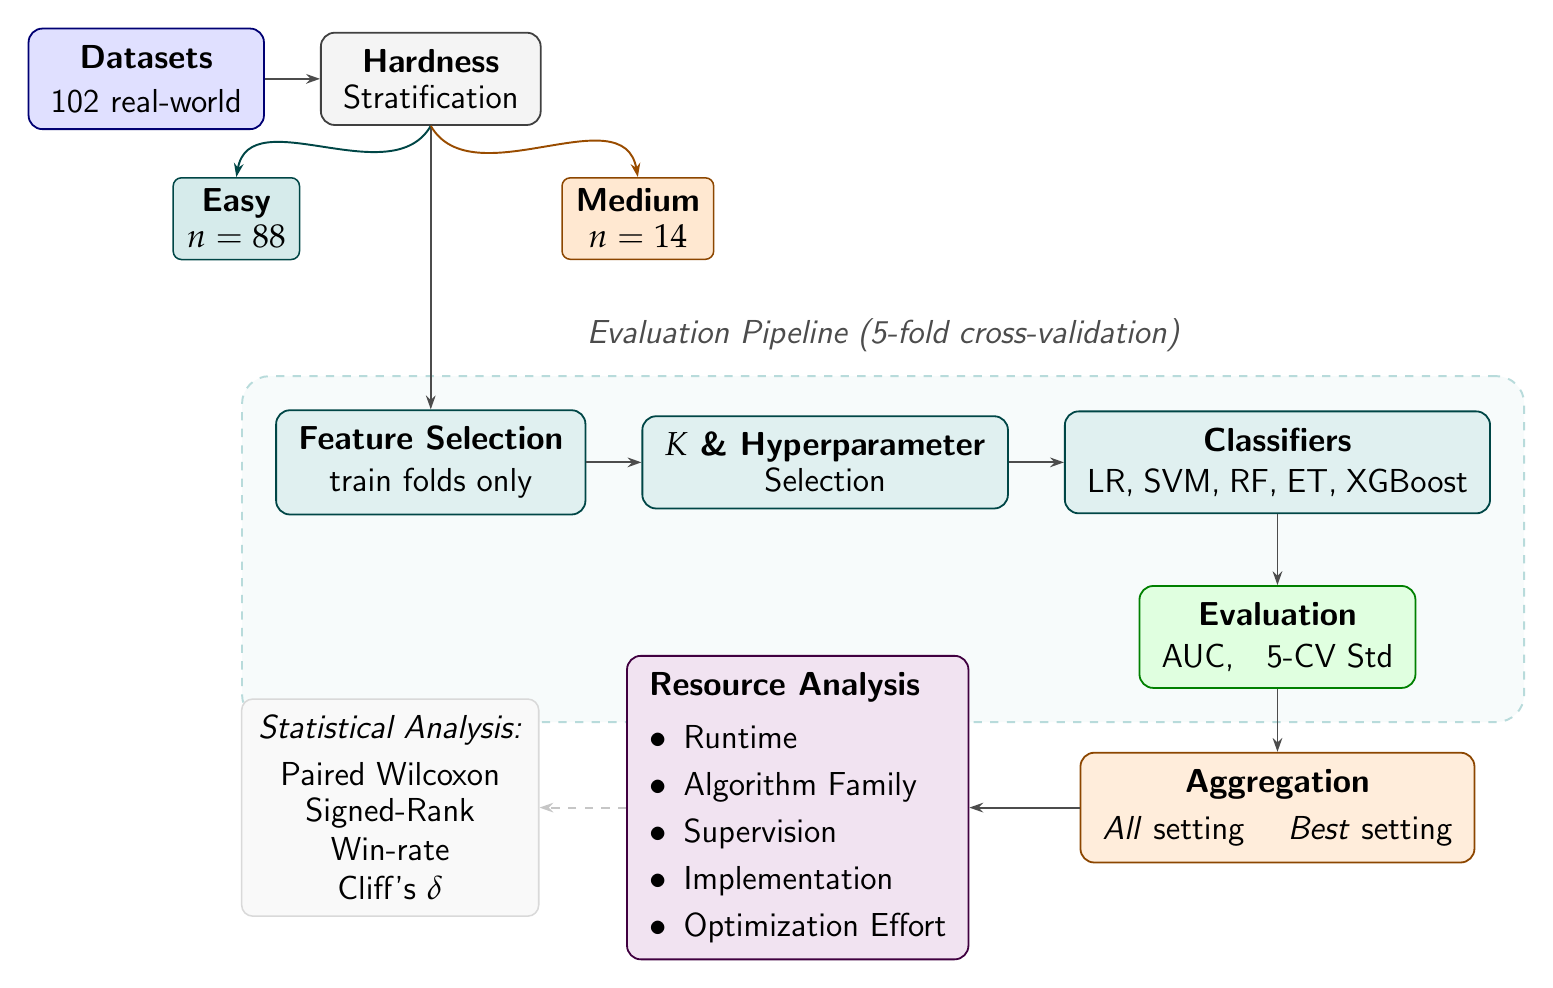
\begin{tikzpicture}[
  N/.style={
    draw, rounded corners=5pt, align=center,
    font=\large\sffamily, inner xsep=8pt, inner ysep=6pt,
    minimum height=1.0cm, line width=0.65pt},
  Nblue/.style  ={N, fill=blue!12,   draw=blue!45!black},
  Nteal/.style  ={N, fill=teal!12,   draw=teal!55!black},
  Ngreen/.style ={N, fill=green!12,  draw=green!50!black},
  Norange/.style={N, fill=orange!14, draw=orange!55!black},
  Npurple/.style={N, fill=violet!11, draw=violet!50!black},
  Ngray/.style  ={N, fill=gray!9,    draw=gray!50!black},
  Etag/.style={
    draw=teal!55!black, fill=teal!16, rounded corners=3pt, align=center,
    font=\large\sffamily\bfseries,
    inner xsep=5pt, inner ysep=4pt, line width=0.55pt},
  Mtag/.style={
    draw=orange!55!black, fill=orange!18, rounded corners=3pt, align=center,
    font=\large\sffamily\bfseries,
    inner xsep=5pt, inner ysep=4pt, line width=0.55pt},
  arr/.style={
    ->, >={Stealth[length=5pt,width=3.5pt]},
    draw=gray!60!black, line width=0.7pt},
  ann/.style={font=\large\sffamily, text=gray!65!black},
  phd/.style={font=\large\sffamily\itshape, text=gray!60!black},
]

%% ROW 1
\node[Nblue, minimum width=2.2cm] (D)
  {\textbf{Datasets}\\[2pt]102 real-world};

\node[Ngray, minimum width=2.6cm, right=0.7cm of D] (HS)
  {\textbf{Hardness}\\[-1pt]Stratification};

\node[Etag, below left=0.65cm and 0.25cm of HS]  (easy)
  {Easy\\[-1pt]$n=88$};
\node[Mtag, below right=0.65cm and 0.25cm of HS] (med)
  {Medium\\[-1pt]$n=14$};

%% ROW 2
\node[Nteal, minimum width=2.6cm, below=3.6cm of HS] (FS)
  {\textbf{Feature Selection}\\[1pt]train folds only};

\node[Nteal, minimum width=2.9cm, right=0.7cm of FS] (KHP)
  {\textbf{$K$ \& Hyperparameter}\\[-1pt]Selection};

\node[Nteal, minimum width=3.0cm, right=0.7cm of KHP] (CLF)
  {\textbf{Classifiers}\\[1pt]LR,\;SVM,\;RF,\;ET,\;XGBoost};

\node[Ngreen, minimum width=2.8cm, below=0.9cm of CLF] (EVAL)
  {\textbf{Evaluation}\\[1pt]AUC,\quad 5-CV Std};

%% LOWER PART
\node[Norange, minimum width=3.0cm, below=0.8cm of EVAL] (AGG)
  {\textbf{Aggregation}\\[3pt]
   \textit{All}~setting \quad \textit{Best}~setting};

\node[Npurple, minimum width=3.4cm,
      font=\large\sffamily, align=left,
      left=1.4cm of AGG] (RES)
  {\textbf{Resource Analysis}\\[5pt]
   $\bullet$\enspace Runtime\\[3pt]
   $\bullet$\enspace Algorithm Family\\[3pt]
   $\bullet$\enspace Supervision\\[3pt]
   $\bullet$\enspace Implementation\\[3pt]
   $\bullet$\enspace Optimization Effort};

\node[draw=gray!30, rounded corners=4pt, fill=gray!5, line width=0.55pt,
      font=\large\sffamily, align=center, inner sep=6pt,
      minimum width=3.0cm, left=1.1cm of RES] (STAT)
  {\textit{Statistical Analysis:}\\[3pt]
   Paired Wilcoxon\\[-1pt]Signed-Rank\\
   Win-rate\\
   Cliff's~$\delta$};

%% ARROWS
\draw[arr] (D) -- (HS);
\draw[arr] (HS.south) -- (FS.north);
\draw[arr, teal!55!black]   (HS.south) to[out=240,in=80]  (easy.north);
\draw[arr, orange!60!black] (HS.south) to[out=300,in=100] (med.north);
\draw[arr] (FS)  -- (KHP);
\draw[arr] (KHP) -- (CLF);
\draw[arr] (CLF.south) -- (EVAL.north);
\draw[arr] (EVAL.south) -- (AGG.north);
\draw[arr] (AGG.west) -- (RES.east);
\draw[arr, dashed, gray!45] (RES.west) -- (STAT.east);

%% GROUP BOX
\begin{scope}[on background layer]
  \node[
    draw=teal!28, dashed, rounded corners=10pt,
    line width=0.7pt, fill=teal!3, inner sep=12pt,
    fit=(FS)(KHP)(CLF)(EVAL)
  ] (cvbox) {};
\end{scope}
\node[phd, above=5pt of cvbox.north]
  {Evaluation Pipeline (5-fold cross-validation)};

\end{tikzpicture}%
}
\caption{Evaluation pipeline for resource-aware feature selection.
A total of 102 real-world datasets are stratified by hardness
\citep{elmakias2025choosing} into {Easy} ($n=88$) and
{Medium} ($n=14$) groups.
Within stratified 5-fold cross-validation, feature selection,
including the choice of $K$ and hyperparameters, is performed
exclusively on training folds to prevent leakage.
Selected features are evaluated using five classifiers
(LR, SVM, RF, ET, XGBoost), with performance measured by AUC
and cross-validation variability.
Results are aggregated under two regimes—\emph{All} (all configurations)
and \emph{Best} (per-dataset optimal configuration)—and analyzed
across five resource dimensions using paired Wilcoxon tests,
win rates, and Cliff's~$\delta$.}
\label{fig:fs_pipeline}
\end{figure}
% \FloatBarrier

\begin{figure*}[t]
\centering
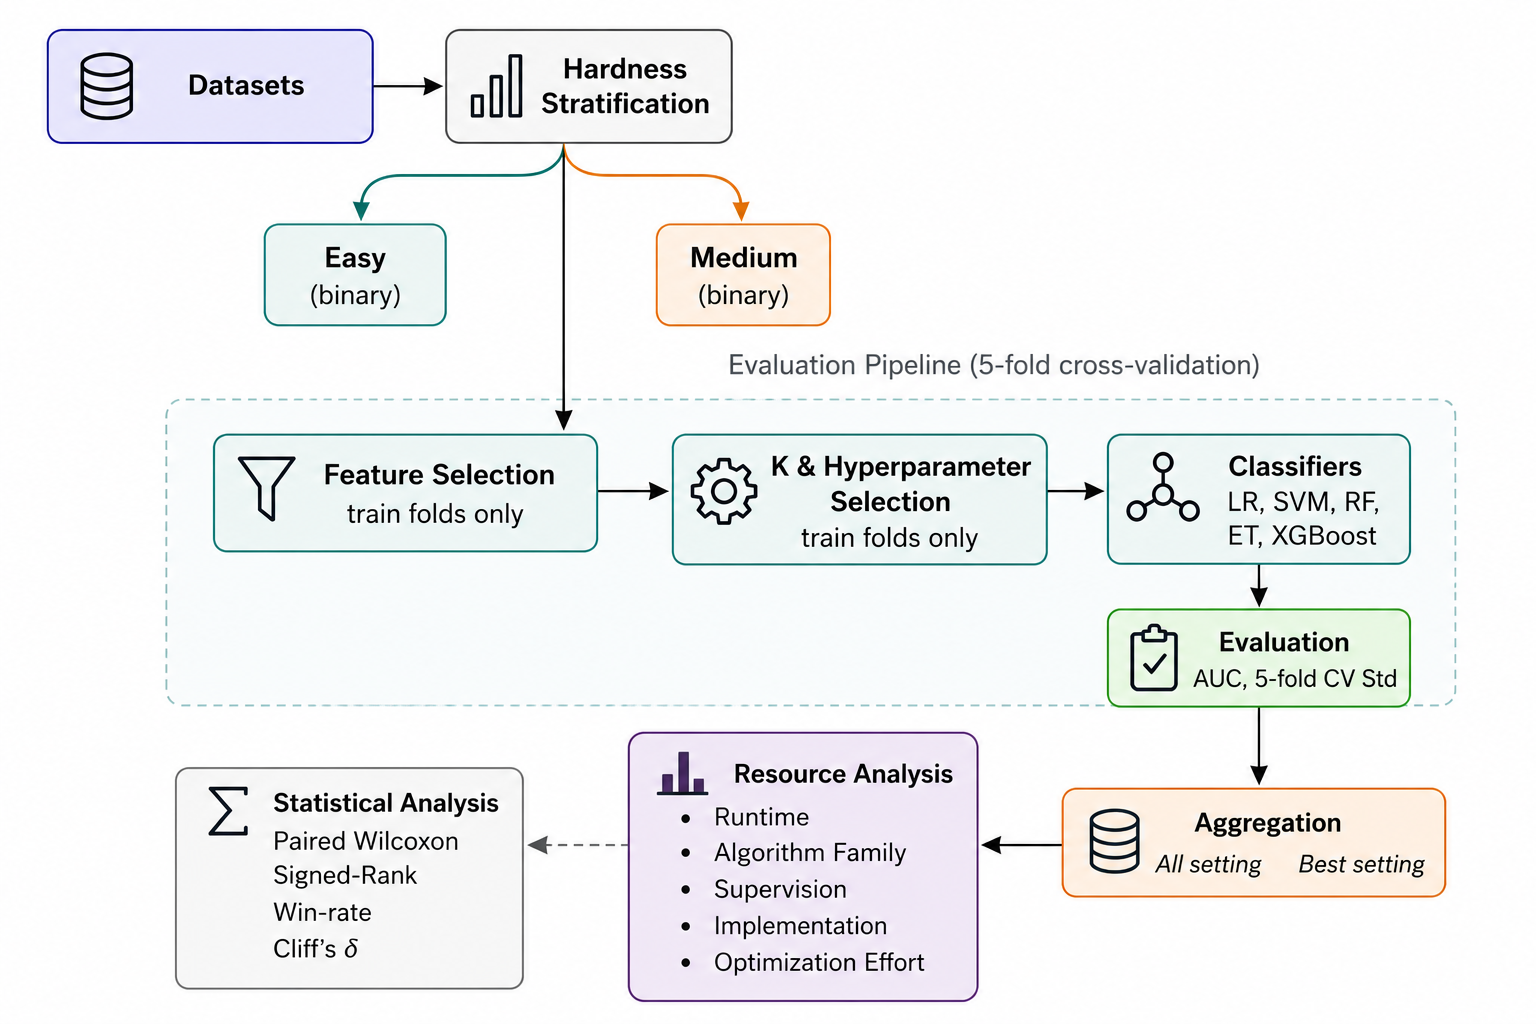
\includegraphics[width=\textwidth]{assets/pipelne_fig.png}
\caption{Evaluation pipeline for resource-aware feature selection.
A total of 102 real-world datasets are stratified by hardness
\citep{elmakias2025choosing} into {Easy} ($n=84$) and
{Medium} ($n=18$) groups.
Within stratified 5-fold cross-validation, feature selection,
including the choice of $K$ and hyperparameters, is performed
exclusively on training folds to prevent leakage.
Selected features are evaluated using five classifiers
(LR, SVM, RF, ET, XGBoost), with performance measured by AUC
and cross-validation variability.
Results are aggregated under two regimes---\emph{All} (all configurations)
and \emph{Best} (per-dataset optimal configuration)---and analyzed
across five resource dimensions using paired Wilcoxon tests,
win rates, and Cliff's~$\delta$.}
\label{fig:fs_pipeline}
\end{figure*}


\subsection{Evaluation Pipeline}

Our evaluation pipeline follows the principles introduced in \cite{elmakias2025choosing}, but is adapted to assess FS algorithms rather than dataset difficulty. For each dataset, we evaluate FS in a downstream classification setting using five common classifiers: Logistic Regression (LR), Support Vector Machine with RBF kernel (SVM), Random Forest (RF), Extremely Randomized Trees (ET), and XGBoost.

Each FS algorithm is applied within a stratified 5-fold cross-validation framework. In every fold:
\begin{enumerate}
    \item The training split is used to fit the FS algorithm.
    \item A subset of $K$ features is selected, with $K \in \{1,5,30,60\}$.
    \item The same selected features are applied to the held-out test split.
    \item Each classifier is trained on the selected training features and evaluated on the selected test features.
    \item Runtime of the FS step only and predictive performance are recorded.
\end{enumerate}

The selected values of $K$ are intended to cover a practical range from very sparse selections ($K=1,5$) to moderate-dimensional subsets ($K=30,60$), while keeping the search space feasible across 37 algorithms, 102 datasets, and multiple classifiers. For datasets with fewer than $K$ available features, the maximum feasible number of features is used.

Importantly, feature selection itself is always fitted only on the training split of each fold. The \emph{Best} setting described below is not a nested-validation estimate of deployment performance; rather, it is a post-hoc benchmark summary used to estimate the potential value of systematic configuration search within each resource category. We therefore interpret \emph{Best} as an upper-bound or oracle-style comparison, not as an unbiased estimate of what a fully nested model-selection pipeline would achieve on a new dataset.

\subsection{Resource Dimensions}\label{sec:resource_dimensions}

We evaluate FS methods through several practical resource dimensions. The purpose is not to produce a single global ranking of algorithms, but to ask whether investing more resources along a given axis yields systematic predictive gains.

\paragraph{Predictive performance}
For binary datasets, we use AUC as the primary metric. AUC is threshold-independent and less sensitive to class imbalance than accuracy, enabling comparisons across datasets with different class distributions. It also aligns with the hardness taxonomy of \cite{elmakias2025choosing}. For multiclass datasets, we use a one-vs-rest (OvR) extension of AUC, while acknowledging that multiclass AUC should be interpreted cautiously in absolute terms. Finally, for nearly balanced datasets, defined as those with majority-class proportions between 40\% and 60\%, we repeat the evaluation using classification accuracy, since accuracy is informative when class imbalance is limited.

\paragraph{Runtime}
Runtime is measured as the wall-clock time required by the FS step within each fold. We discretize runtime into three buckets: Fast ($<1$ minute), Moderate (1 minute--1 hour), and Slow ($>1$ hour). Since runtime naturally depends on dataset size and structure, assigning a single runtime category to an algorithm requires aggregation across datasets. For each algorithm, we collect all executions over all datasets and assign it to a runtime bucket if at least 60\% of its runs fall within that bucket. If no bucket reaches this threshold, the algorithm is labeled as \emph{Mixed}. Mixed algorithms are reported in Table~\ref{tab:FS_algs} but excluded from the main runtime comparison to preserve a clean ordinal comparison between Fast, Moderate, and Slow categories. This affects seven algorithms; we therefore interpret runtime conclusions as applying to algorithms with a dominant runtime profile.

\paragraph{Implementation effort}
We distinguish between methods available in standard libraries and those implemented from research papers. Library implementations are typically maintained, tested, and easier to deploy, whereas research-code implementations may require adaptation, debugging, and additional effort to understand and justify. We therefore treat implementation source as a practical proxy for engineering and adoption cost.

\paragraph{Algorithm family}
Each FS method is categorized as filter, wrapper, embedded, ensemble, or hybrid, following the standard taxonomy in the FS literature. This dimension is methodological, but also practically meaningful: filters are typically lightweight and easy to tune; wrappers repeatedly train downstream models and are often computationally expensive; embedded methods integrate selection into model fitting; ensembles aggregate multiple models; and hybrids combine multiple stages. This categorization allows comparison with prior survey-based conclusions and serves as a coarse proxy for methodological complexity.

\paragraph{Supervision}
We distinguish between supervised and unsupervised FS methods. Supervision is often not a tunable resource in practice, since labels are either available or not. Nevertheless, it is relevant for decision-making: if supervised FS yields clear gains, investing in label collection or label quality may be justified; if not, unsupervised methods may provide a more scalable alternative.

\paragraph{Optimization effort}
To quantify the value of practical tuning, we define two evaluation settings. Here, optimization effort is understood broadly: it includes trying several FS algorithms within the same resource category, evaluating multiple values of $K$, and using recommended hyperparameter settings when such settings are provided by standard implementations or public repositories. It does not refer to exhaustive nested grid search over all possible hyperparameters. Such a search may be feasible for a practitioner working with a single dataset, but it is impractical at the scale of our benchmark and would make comparisons across 37 algorithms and 102 datasets prohibitively expensive.

In the \emph{All} setting, we include all runs across evaluated values of $K$ and recommended hyperparameter settings. Although this may appear to be high effort, its purpose is to capture the variability that arises when configurations are chosen without systematic selection. In the \emph{Best} setting, we retain, for each dataset and resource category, the configuration that achieves the highest cross-validated performance. This approximates a practitioner who searches over several algorithms, values of $K$, and reasonable configurations under a fixed resource budget, while also providing an oracle-style estimate of the potential gain from such search.

Together, \emph{All} and \emph{Best} separate two questions: whether FS is stable under arbitrary configuration choices, and how much can be gained by deliberate search within a realistic configuration space.

\subsection{Aggregation, Visualization, and Statistical Analysis}\label{sec:statistical_analysis}

For each resource dimension, we group experiments by the corresponding resource category. For example, in the runtime analysis, FS runs are grouped into Fast, Moderate, and Slow buckets; in the implementation analysis, runs are grouped into Library and research-code implementations. In the binary setting, all comparisons are performed separately for Easy and Medium datasets. In the multiclass and nearly balanced settings, the number of Medium datasets is too small for reliable stratification (three in the multiclass setting and a small number in the nearly balanced subset), so datasets are analyzed jointly and comparisons are made only across resource categories.

We summarize performance using boxplots that report the distribution of mean 5-fold cross-validated performance across datasets and resource categories. The median serves as a compact summary, while the spread captures variability across datasets, algorithms, values of $K$, and configurations. We also report a secondary stability measure: the average standard deviation across the five cross-validation folds, which captures sensitivity to train/test splits rather than sensitivity to algorithmic or configuration choices.

To assess whether additional resource investment yields consistent gains, we perform paired within-dataset comparisons. For each dataset, we compare the best-performing configuration in a higher-cost category with the corresponding best-performing configuration in the lower-cost category. The unit of inference is the dataset, not the individual algorithm--configuration run. This dataset-level aggregation avoids treating correlated runs on the same dataset as independent observations.

Formally, for a higher-cost category $X$ and a lower-cost category $Y$, we test whether the paired differences $X-Y$ are systematically positive using a one-sided Wilcoxon signed-rank test \cite{wilcoxon1945individual,demsar2006statistical}. We complement this test with the win-rate $\Pr[X>Y]$ and Cliff's $\delta=\Pr[X>Y]-\Pr[Y>X]$ as descriptive measures of dominance. These quantities distinguish between statistically detectable differences and practically meaningful effects. We report conventional Cliff's $\delta$ thresholds only as rough descriptive guidance: $|\delta| < 0.147$ (negligible), $0.147 \leq |\delta| < 0.330$ (small), $0.330 \leq |\delta| < 0.474$ (medium), and $|\delta| \geq 0.474$ (large) \cite{romano2006appropriate}.

Table~\ref{tab:stat_tests_summary} summarizes the statistical tests and descriptive quantities used in the analysis.

\begin{table}[t]
\centering
\footnotesize
\renewcommand{\arraystretch}{1.2}
\setlength{\tabcolsep}{4pt}

\begin{tabularx}{\linewidth}{
>{\raggedright\arraybackslash}p{2.5cm}
>{\raggedright\arraybackslash}p{3.2cm}
>{\raggedright\arraybackslash}p{2.8cm}
>{\raggedright\arraybackslash}X}
\toprule
\textbf{Test/Metric} & \textbf{Applied To} & \textbf{Type} & \textbf{What It Measures} \\
\midrule

Wilcoxon Signed-Rank
& Paired comparisons (per dataset)
& Nonparametric, paired
& Whether $\mathrm{median}(X - Y) > 0$ within datasets \\

Win-rate $\Pr[X > Y]$
& Paired comparisons
& Descriptive statistic
& Frequency with which higher-cost wins \\

Cliff's Delta ($\delta$)
& Paired comparisons
& Effect size
& $\Pr[X > Y] - \Pr[Y > X]$; measures dominance magnitude \\

\bottomrule
\end{tabularx}

\caption{Summary of statistical tests and metrics used in the analysis. All primary comparisons use paired within-dataset tests to control for dataset-level heterogeneity.}
\label{tab:stat_tests_summary}
\end{table}

\section{Results}\label{sec:results}
We now present a detailed analysis of applying our methodology for 37 FS algorithms across the 63 binary benchmark datasets and 39 multiclass datasets. All experiments were conducted on a high-performance compute environment comprising (i)~10$\times$ NVIDIA RTX A5000 GPUs, (ii)~512~GB RAM, and (iii)~2$\times$ AMD EPYC 7443 CPUs (24 cores each).

Our goal in this section is to quantify the cost-benefit trade-offs associated with each resource. We begin with runtime, the most direct and commonly considered resource.

\subsection{Overview of the Results}\label{sec:results_overview}

Before turning to each resource dimension in detail, we summarize the logic of the empirical analysis, Table \ref{tab:results_tests_overview}. The Results section answers two complementary questions. First, how much does practical optimization effort matter when applying FS? Second, after optimization, is there evidence that higher-cost resource categories systematically outperform lower-cost ones? Throughout, ``no dominance'' is interpreted conservatively as lack of evidence that the higher-cost category consistently improves performance, not as proof of equivalence.

\begin{table}[h!]
\centering
\scriptsize
\setlength{\tabcolsep}{3pt}
\renewcommand{\arraystretch}{1.08}
\begin{tabularx}{\linewidth}{p{2.6cm} p{2.2cm} p{3.8cm} X}
\toprule
\textbf{Analysis} & \textbf{Section} & \textbf{Comparison} & \textbf{Purpose} \\
\midrule

Optimization effort
& Sec.~\ref{sec:runtime_results}
& \emph{All} vs.\ \emph{Best}, relative to No-FS
& Tests whether poor FS performance reflects FS itself or insufficient search over algorithms, $K$, and configurations. \\

Runtime
& Sec.~\ref{sec:runtime_results}
& Fast vs.\ Moderate vs.\ Slow
& Assesses whether additional computation yields better predictive performance or stability. \\

Method family
& Sec.~\ref{sec:family_results}
& Filter, Embedded, Wrapper, Ensemble, Hybrid
& Tests whether more complex FS families outperform simpler families after optimization. \\

Supervision
& Sec.~\ref{sec:supervision_results}
& Supervised vs.\ Unsupervised
& Evaluates whether label-dependent FS yields consistent gains over unsupervised alternatives. \\

Implementation effort
& Sec.~\ref{sec:implementation_results}
& Library vs.\ Research-code methods
& Assesses whether harder-to-deploy implementations provide performance or stability benefits. \\

Multiclass \& nearly-balanced datasets
& Sec.~\ref{sec:multiclass_balanced_results}
& Repeating analysis for these datasets
& Assessing whether results extend to multiclass; for nearly balanced data, we use accuracy, checking generalization using other metrics. \\




\bottomrule
\end{tabularx}
\caption{Summary of the analyses reported in the Results section.}
\label{tab:results_tests_overview}



\end{table}

\subsection{Summary of Resource Dominance}\label{sec:summary_dominance}

Table~\ref{tab:wilcoxon_summary} synthesizes the key findings from our paired within-dataset comparisons across all four resource dimensions. In most cases, higher-cost resources do not consistently outperform lower-cost alternatives. For runtime, fast methods significantly dominate computationally expensive ones. For implementation effort, library methods consistently outperform research-code implementations. For method families, Filter methods match or exceed more complex alternatives, with Hybrid methods being significantly dominated. Supervision is the only dimension where higher-cost (supervised) methods provide consistent advantages, though this effect weakens substantially for Medium datasets.

\begin{table}[h]
\centering
\scriptsize
\setlength{\tabcolsep}{4pt}
\begin{tabularx}{\linewidth}{|l|X|X|}
\hline
\textbf{Resource Dimension} & \textbf{Easy Datasets} & \textbf{Medium Datasets} \\
\hline
Runtime & Fast $\succ$ Slow ($p{\approx}1.0$, $\delta{=}{-}0.72$, WR\,2.3\%); Fast $\succ$ Moderate & Fast $\succ$ Slow ($p{=}1.0$, $\delta{=}{-}1.0$, WR\,0\%); similar vs.\ Moderate \\
\hline
Method Family & Filter $\succ$ Hybrid ($p{\approx}0.99$, $\delta{=}{-}0.19$, WR\,33\%); no other family $\succ$ Filter & Filter $\succ$ Hybrid ($p{=}1.0$, $\delta{=}{-}1.0$, WR\,0\%); no other family $\succ$ Filter \\
\hline
Supervision & Supervised $\succ$ Unsupervised ($p{\approx}2.9{\times}10^{-8}$, $\delta{=}0.80$, WR\,82\%) & Weak advantage for Supervised ($p{\approx}0.028$, $\delta{=}0.64$, WR\,82\%); effect weaker than Easy \\
\hline
Implementation & Library $\succ$ Research Code ($p{\approx}0.006$, $\delta{=}0.36$, WR\,58\%) & Library $\succ$ Research Code ($p{\approx}0.016$, $\delta{=}0.64$, WR\,82\%) \\
\hline
\end{tabularx}
\caption{Paired within-dataset dominance tests across resource dimensions. WR = win rate of the higher-cost category; $\delta$ = Cliff's delta; $\succ$ denotes consistent dominance via one-sided Wilcoxon signed-rank test.}
\label{tab:wilcoxon_summary}
\end{table}
%%%%%%%%%%%%%%%%%%%%%%%%%%%%%%%%%%%%%%%%%%%%%%%%%%%%%%%%%%%%%%%%%%%
%%% RUNTIME RESULTS %%%%%%%%%%%%%%%%%%%%%%%%%%%%%%%%%%%%%%%%%%%%%%%
%%%%%%%%%%%%%%%%%%%%%%%%%%%%%%%%%%%%%%%%%%%%%%%%%%%%%%%%%%%%%%%%%%%

\subsection{Runtime: compute investment vs.\ performance}\label{sec:runtime_results}

As part of our goal to derive practical, high-level rules of thumb, we intentionally abstract away from fine-grained runtime differences and group methods into three coarse runtime buckets based on the median runtime per dataset and per $K$: Fast ($\le$ 1 minute), Moderate (between 1 minute and 1 hour), and Slow ($\ge$ 1 hour).

Given the high-end hardware we've used, the reported runtimes should be interpreted as \emph{optimistic lower bounds}. On more typical hardware—such as a single-GPU server, CPU-only desktop, or personal laptop—execution times may be substantially longer, particularly for wrapper-based and deep-learning methods. Detailed execution times for each algorithm--dataset pair are provided in the supplementary material to facilitate reproducibility and comparison.

We begin with the ALL-mode analysis (recall Section~\ref{sec:resource_dimensions} for the distinction between ALL and BEST modes), which reflects a low-effort setting where both the algorithm choice and hyperparameter optimization are not tuned. The relevant results are shown in Figures~\ref{fig:runtime_boxplots}--\ref{fig:stability_runtime}. For Easy datasets, we observe a substantial degradation in AUC relative to the No-FS baseline—on the order of $\sim$7 nominal AUC points (e.g., median $\sim$0.92 for fast vs.\ $\sim$0.99 in Figure~\ref{fig:runtime_boxplots}). A similar, though slightly larger, degradation is also observed for Medium datasets (e.g., $\sim$0.58 vs.\ $\sim$0.69), indicating that naïvely applying feature selection can be detrimental across difficulty levels. While this highlights a key limitation of ALL-mode, we set this observation aside for now and revisit it when analyzing the BEST-mode results.

\begin{figure}[h!]
\centering
\begin{subfigure}{0.48\linewidth}
    \centering
    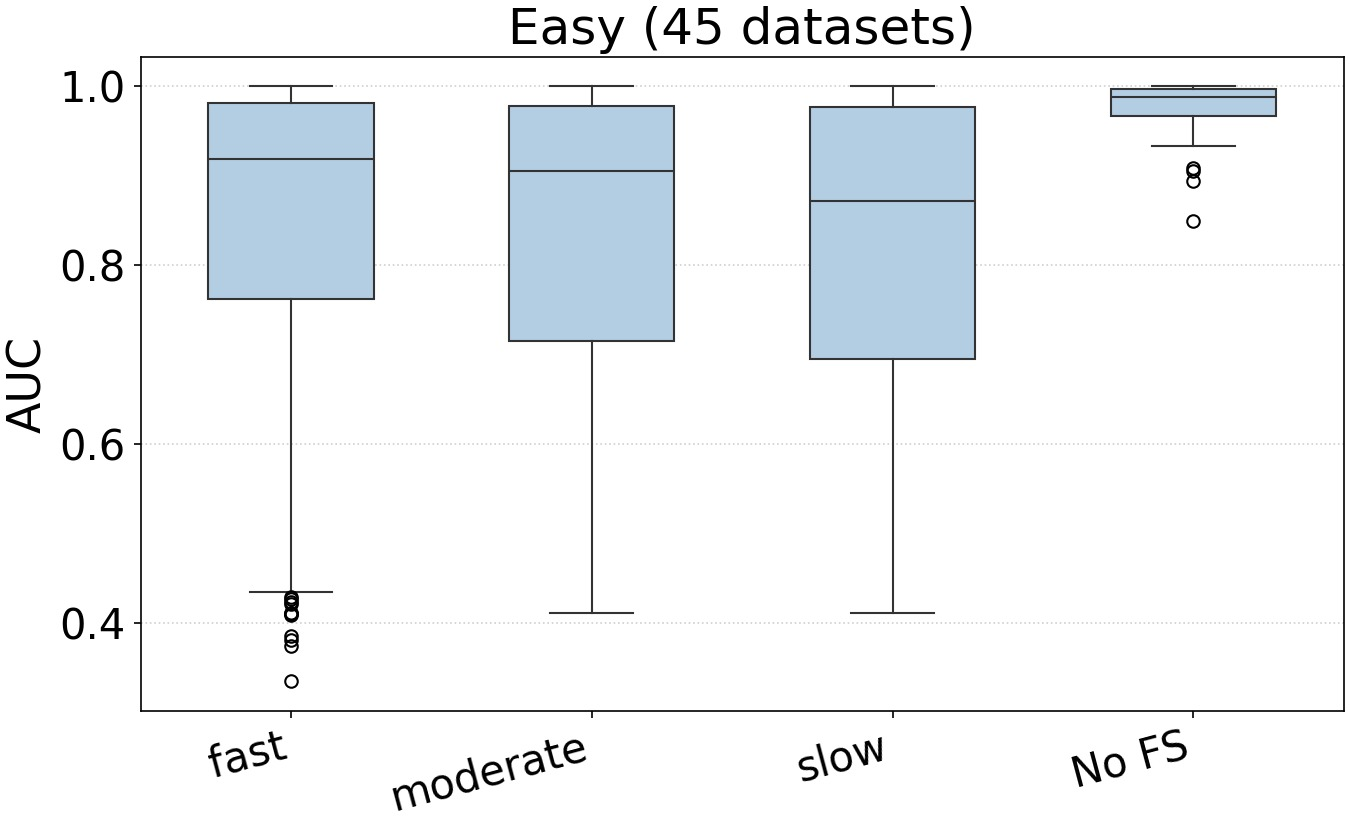
\includegraphics[width=\linewidth]{assets/Dan_Figs/boxplotubset-core_datasets_all_FS_rows_Easy_nDatasets-45.jpg}
    \caption{Easy datasets ($n=45$)}
\end{subfigure}
\hfill
\begin{subfigure}{0.48\linewidth}
    \centering
    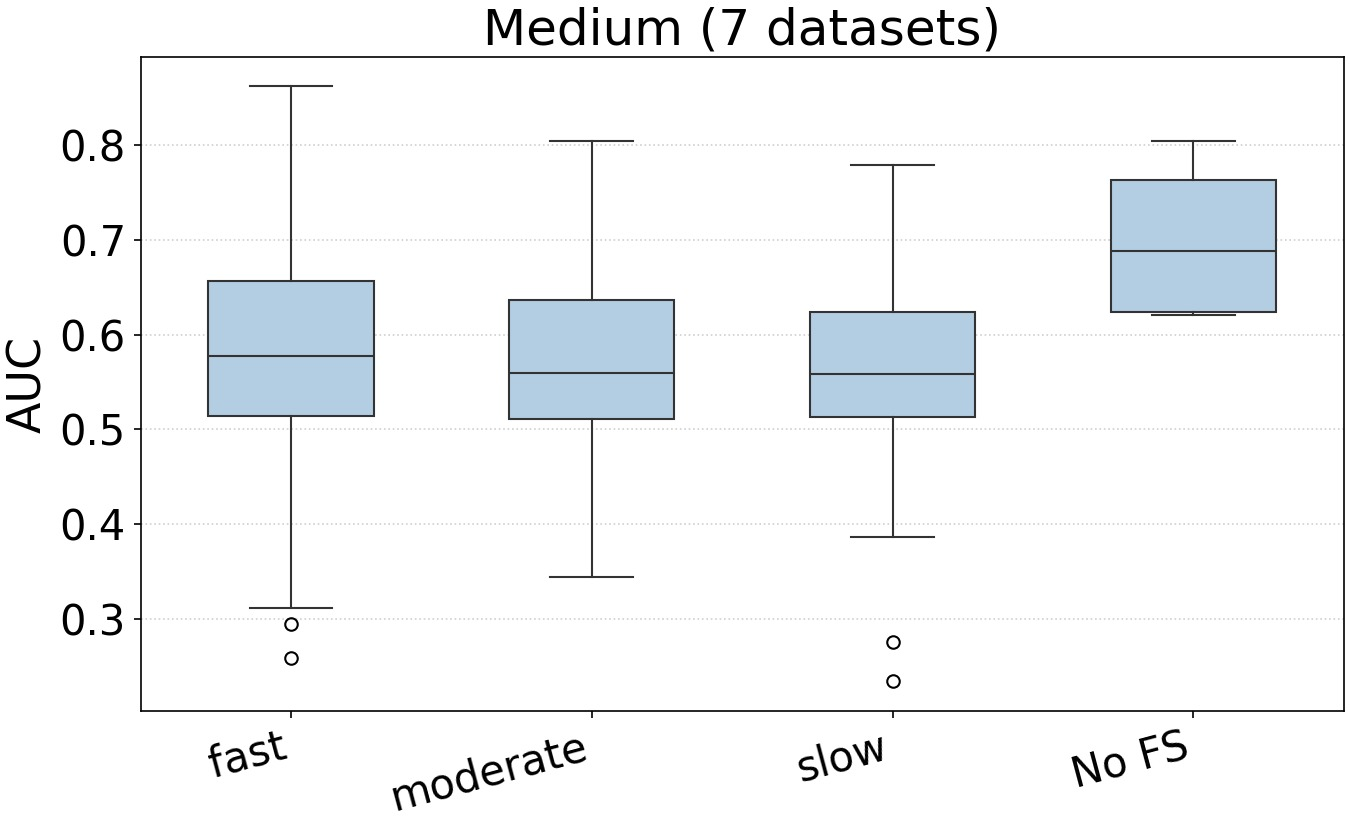
\includegraphics[width=\linewidth]{assets/Dan_Figs/boxplotubset-core_datasets_all_FS_rows_Medium_nDatasets-7.jpg}
    \caption{Medium datasets ($n=7$)}
\end{subfigure}
\caption{
Distribution of ALL-mode cross-validated AUC across runtime buckets and the No-FS baseline. Medians for Easy: 0.919 (fast), 0.905 (moderate), 0.872 (slow), 0.989 (No-FS). Medians for Medium: 0.578 (fast), 0.560 (moderate), 0.558 (slow), 0.688 (No-FS). The visual comparison shows substantial performance degradation from the No-FS baseline when FS is applied without optimization, particularly for slow methods.
}
\label{fig:runtime_boxplots}
\end{figure}

\begin{figure}[h!]
\centering
\begin{subfigure}{0.48\linewidth}
    \centering
    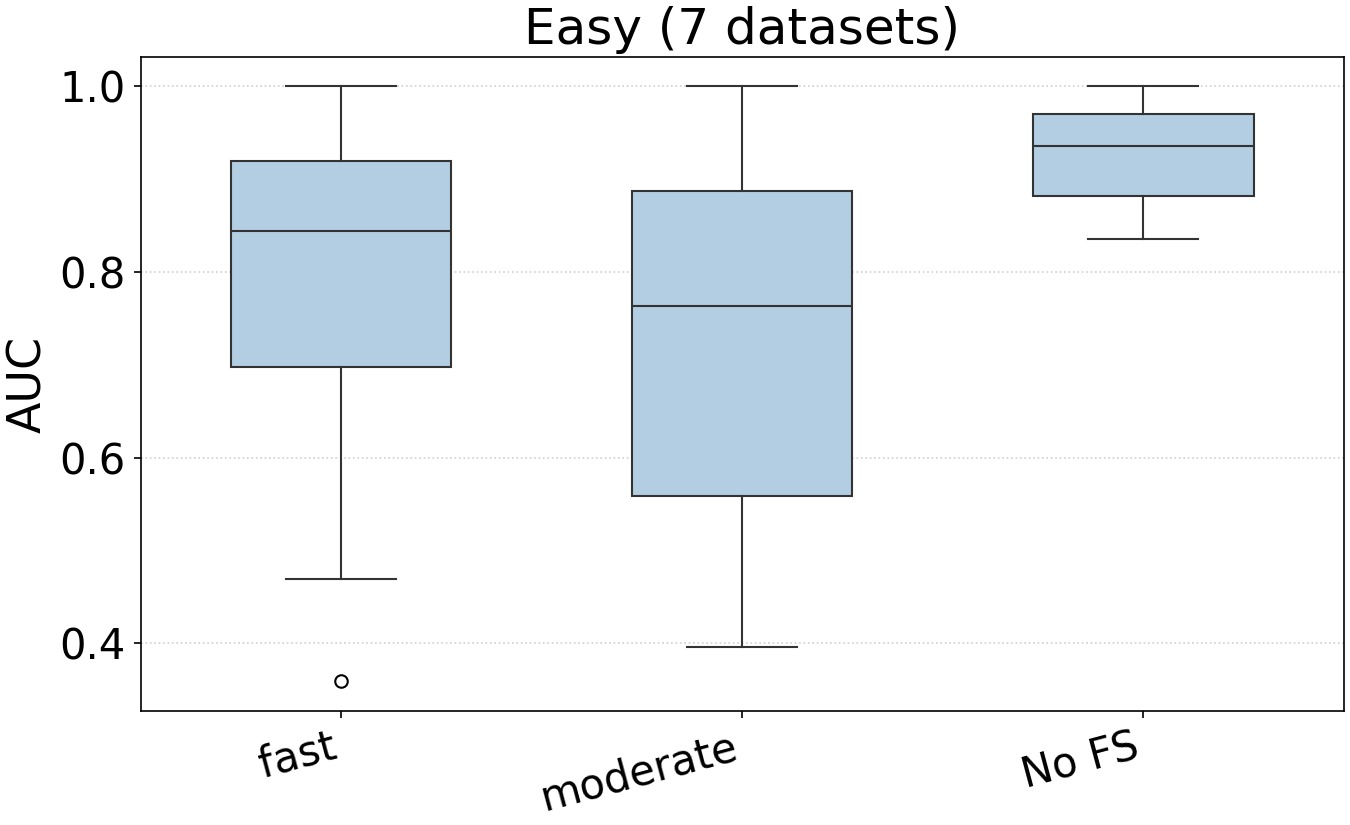
\includegraphics[width=\linewidth]{assets/Dan_Figs/boxplotubset-rem_datasets_fast_moderate_FS_rows_Easy_nDatasets-7.jpg}
    \caption{Easy datasets ($n=7$)}
\end{subfigure}
\hfill
\begin{subfigure}{0.48\linewidth}
    \centering
    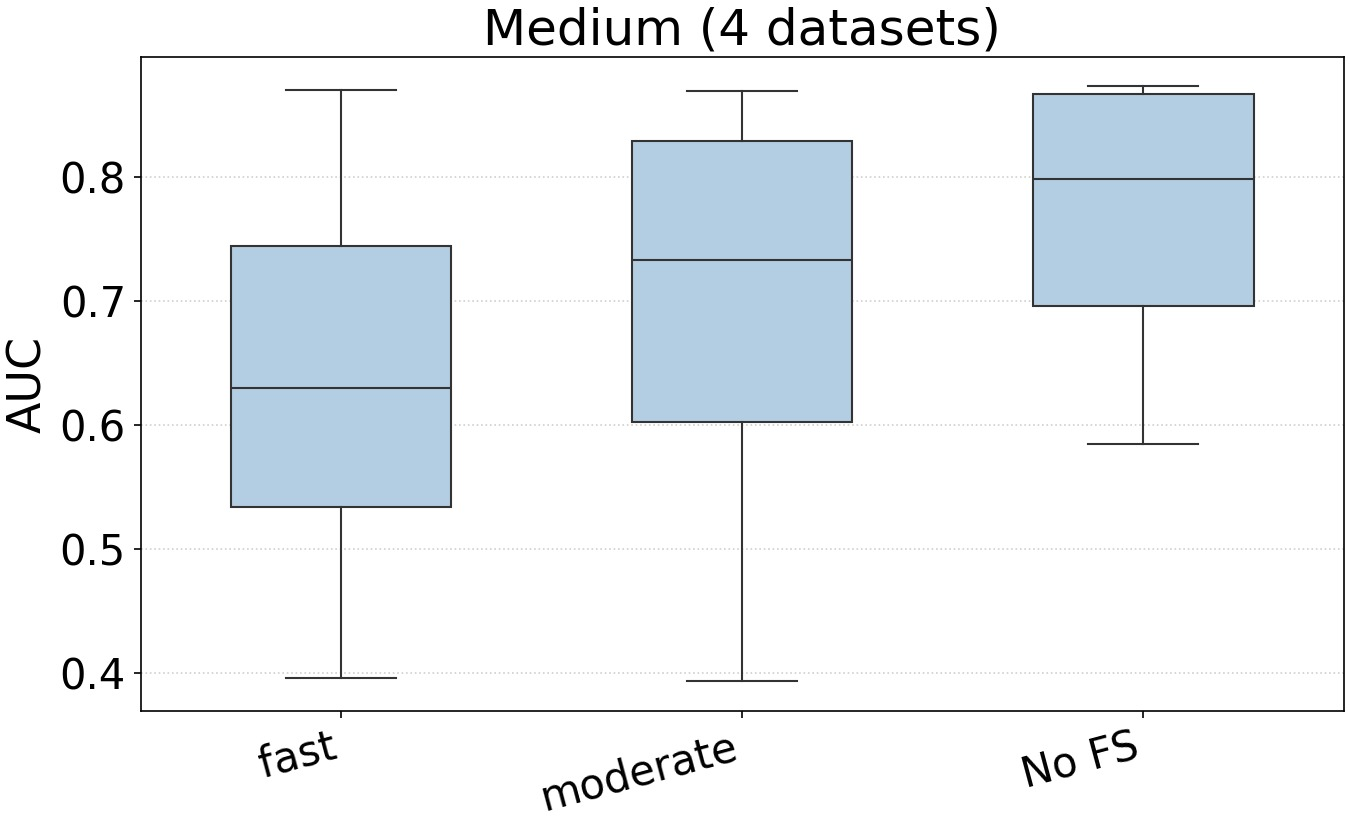
\includegraphics[width=\linewidth]{assets/Dan_Figs/boxplotubset-rem_datasets_fast_moderate_FS_rows_Medium_nDatasets-4.jpg}
    \caption{Medium datasets ($n=4$)}
\end{subfigure}
\caption{
Distribution of ALL-mode cross-validated AUC for datasets with only fast and moderate results available. Medians for Easy: 0.844 (fast), 0.764 (moderate), 0.936 (No-FS). Medians for Medium: 0.630 (fast), 0.733 (moderate), 0.799 (No-FS). The pattern of performance degradation from No-FS persists across this subset.
}
\label{fig:runtime_boxplots_two_groups}
\end{figure}

\begin{figure}[h!]
\centering
\begin{subfigure}{0.48\linewidth}
    \centering
    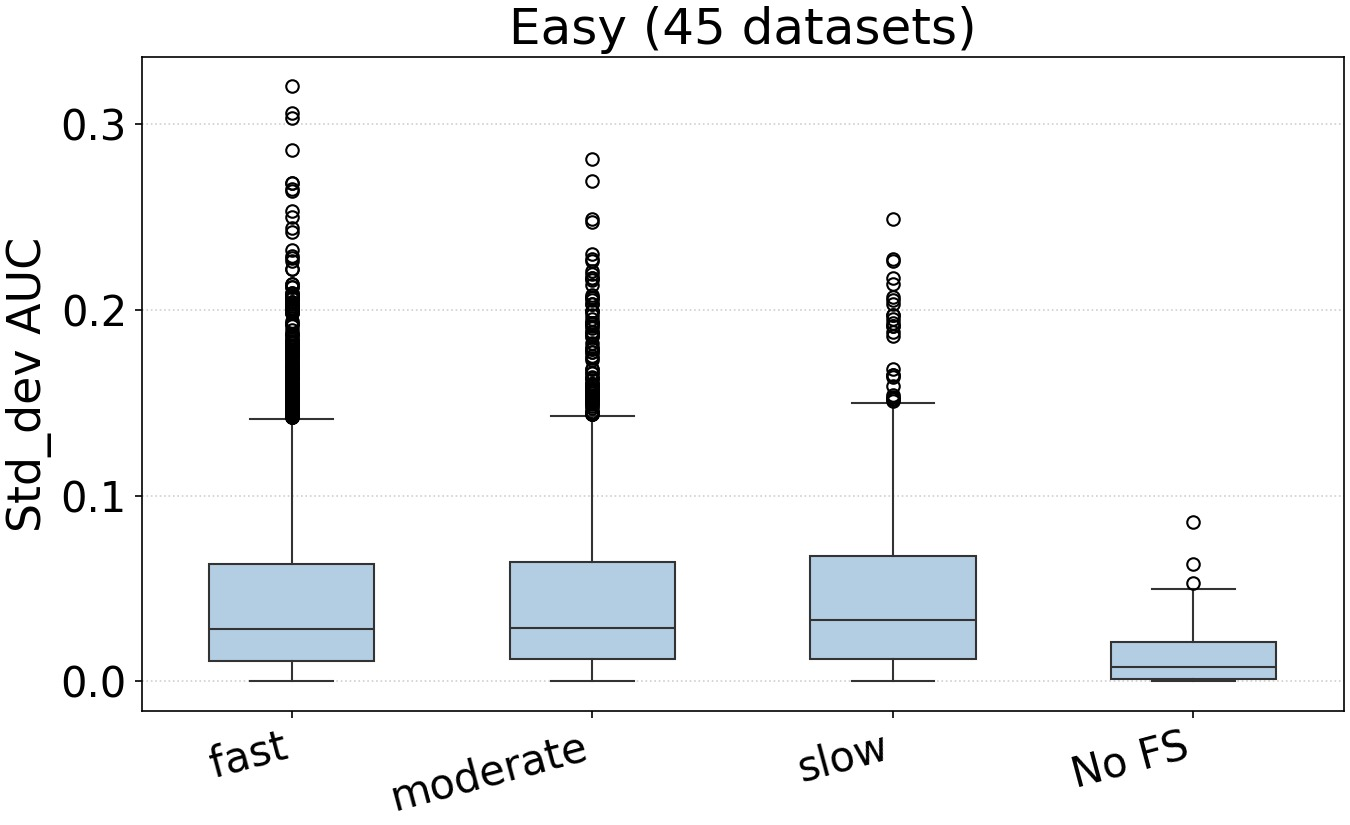
\includegraphics[width=\linewidth]{assets/Dan_Figs/boxplotubset-core_datasets_all_FS_rows_stability_Easy_nDatasets-45.jpg}
    \caption{Easy datasets ($n=45$)}
\end{subfigure}
\hfill
\begin{subfigure}{0.48\linewidth}
    \centering
    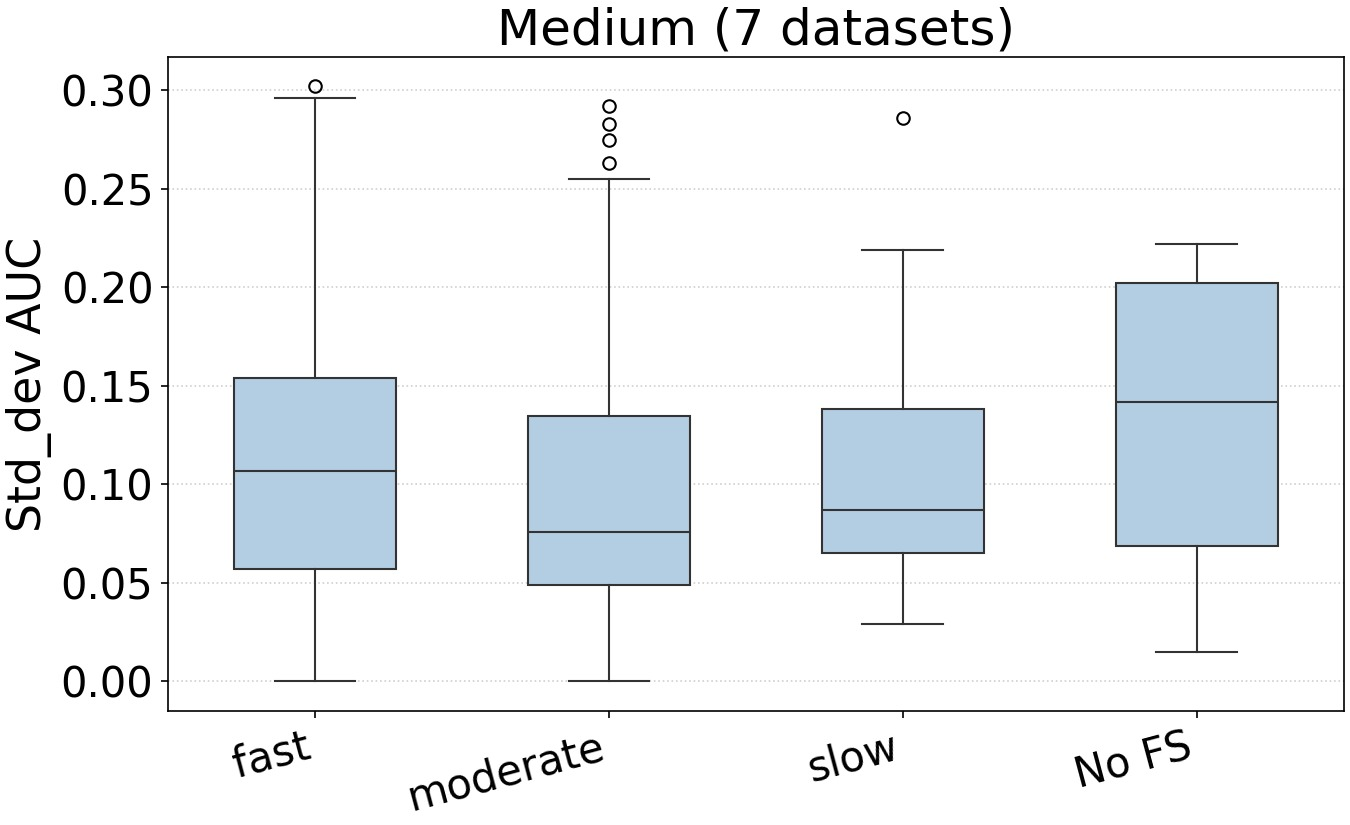
\includegraphics[width=\linewidth]{assets/Dan_Figs/boxplotubset-core_datasets_all_FS_rows_stability_Medium_nDatasets-7.jpg}
    \caption{Medium datasets ($n=7$)}
\end{subfigure}
\caption{
Distribution of ALL-mode cross-validated AUC variability (standard deviation across 5 folds) across runtime buckets and the No-FS baseline. Medians for Easy: 0.028 (fast), 0.029 (moderate), 0.033 (slow), 0.008 (No-FS). Medians for Medium: 0.107 (fast), 0.076 (moderate), 0.087 (slow), 0.142 (No-FS). The No-FS baseline shows the lowest variability for Easy datasets, while Medium datasets exhibit higher variability overall.
}
\label{fig:stability_runtime}
\end{figure}



\begin{figure}[h!]
\centering
\begin{subfigure}{0.48\linewidth}
    \centering
    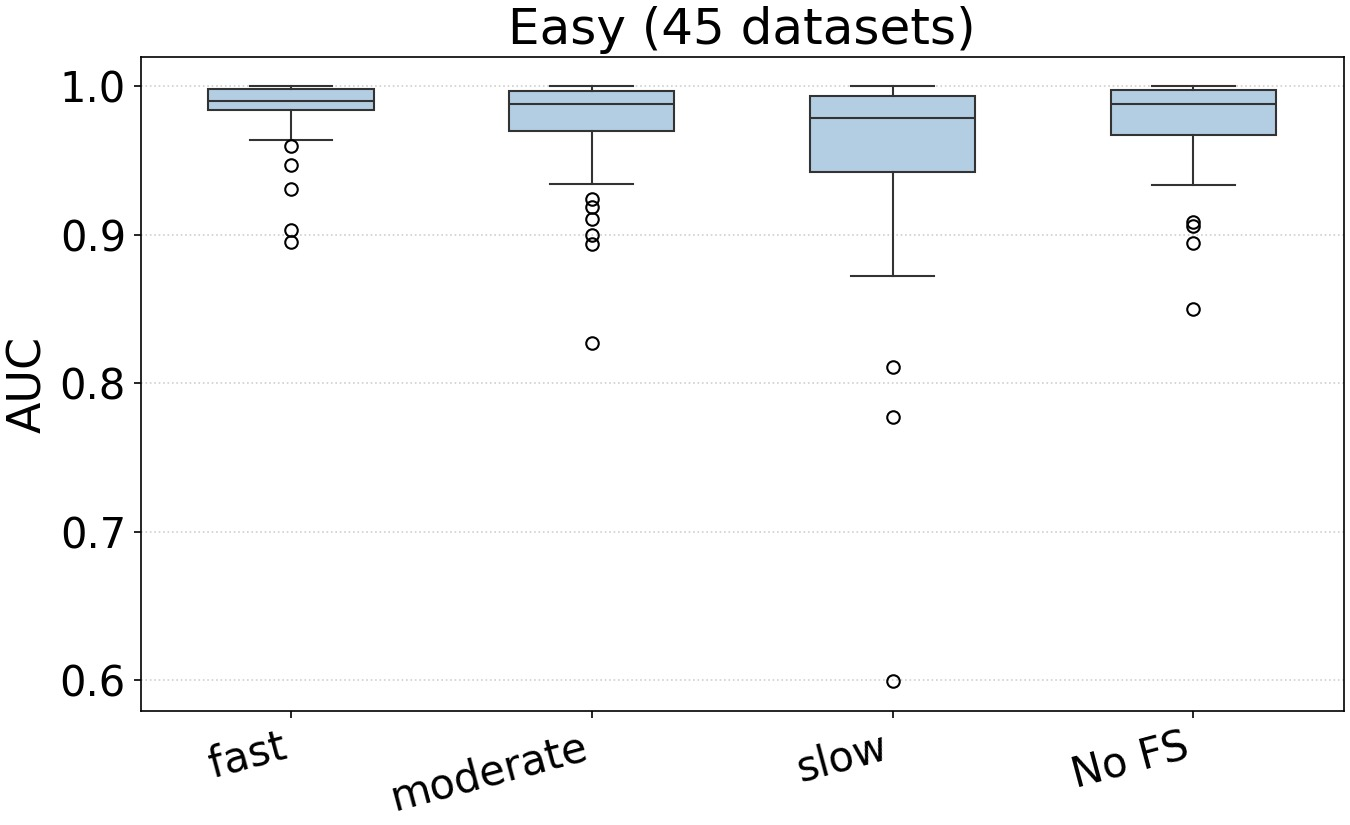
\includegraphics[width=\linewidth]{assets/Dan_Figs/boxplotubset-core_datasets_best_FS_rows_Easy_nDatasets-45.jpg}
    \caption{Easy datasets ($n=45$)}
\end{subfigure}
\hfill
\begin{subfigure}{0.48\linewidth}
    \centering
    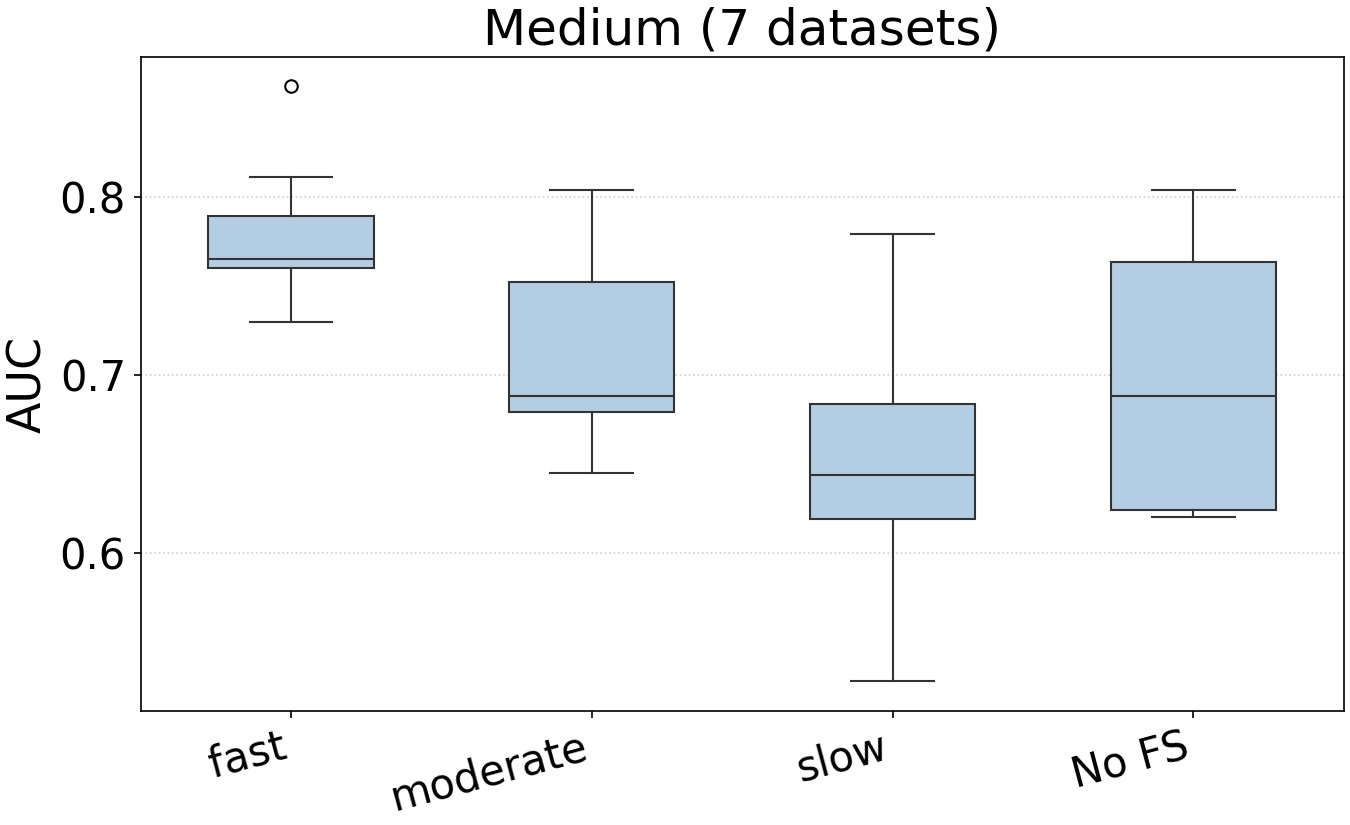
\includegraphics[width=\linewidth]{assets/Dan_Figs/boxplotubset-core_datasets_best_FS_rows_Medium_nDatasets-7.jpg}
    \caption{Medium datasets ($n=7$)}
\end{subfigure}
\caption{
Distribution of BEST-mode cross-validated AUC across runtime buckets and the No-FS baseline. Each point represents the best FS configuration within each runtime bucket per dataset. Medians for Easy: 0.990 (fast), 0.988 (moderate), 0.979 (slow), 0.989 (No-FS). Medians for Medium: 0.765 (fast), 0.688 (moderate), 0.644 (slow), 0.688 (No-FS). Performance recovers to No-FS levels with optimization. Paired within-dataset tests for Easy ($n=45$ with all three buckets): fast significantly outperforms slow (median difference $-0.009$, Cliffs delta $-0.72$, $p \approx 1.0$) and moderate shows no advantage over fast (median difference $-0.001$, Cliffs delta $-0.31$, $p \approx 1.0$). For Medium ($n=7$), fast substantially outperforms slow (median difference $-0.114$, Cliffs delta $-1.0$, $p = 1.0$).
}
\label{fig:best_runtime}
\end{figure}

\begin{figure}[h!]
\centering
\begin{subfigure}{0.48\linewidth}
    \centering
    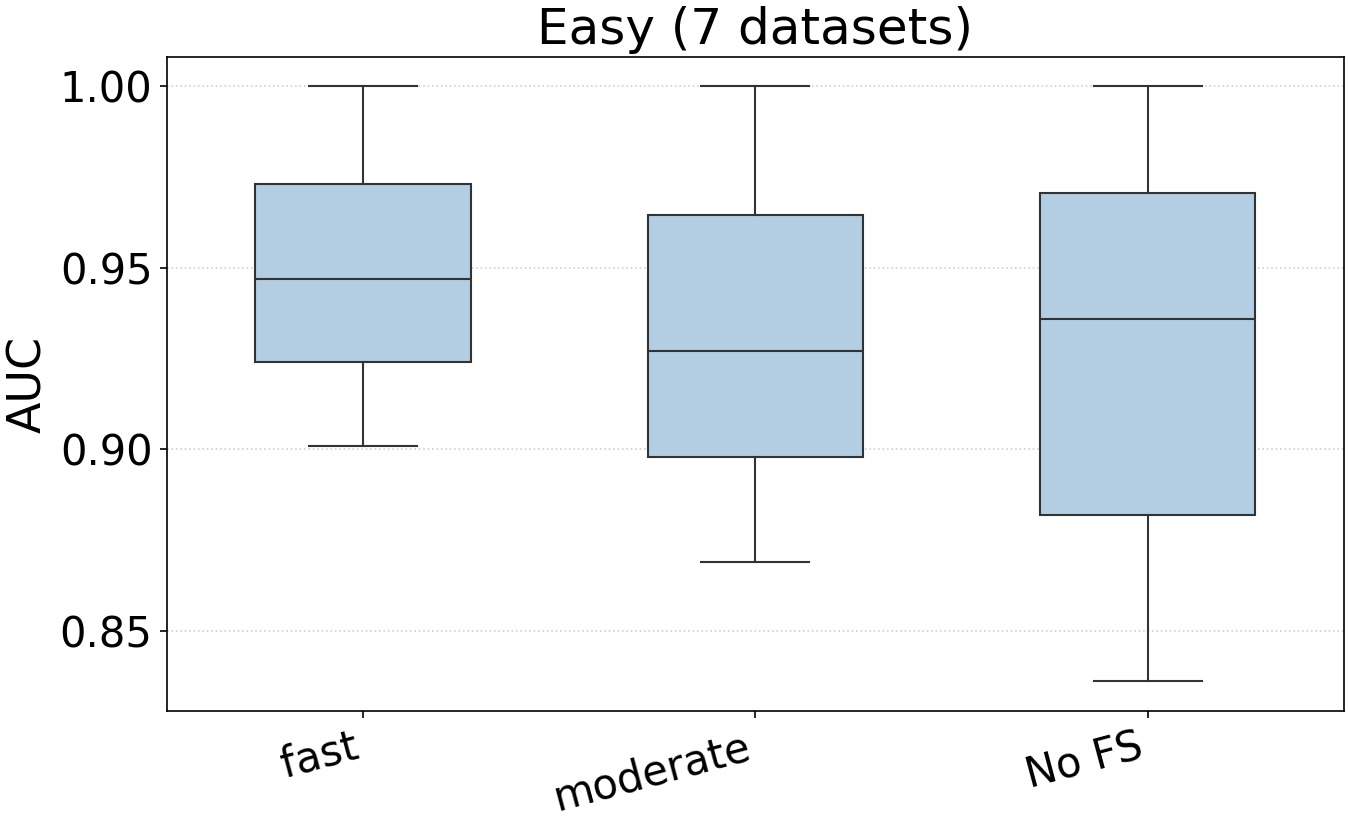
\includegraphics[width=\linewidth]{assets/Dan_Figs/boxplotubset-rem_datasets_fast_moderate_best_FS_rows_Easy_nDatasets-7.jpg}
    \caption{Easy datasets ($n=7$)}
\end{subfigure}
\hfill
\begin{subfigure}{0.48\linewidth}
    \centering
    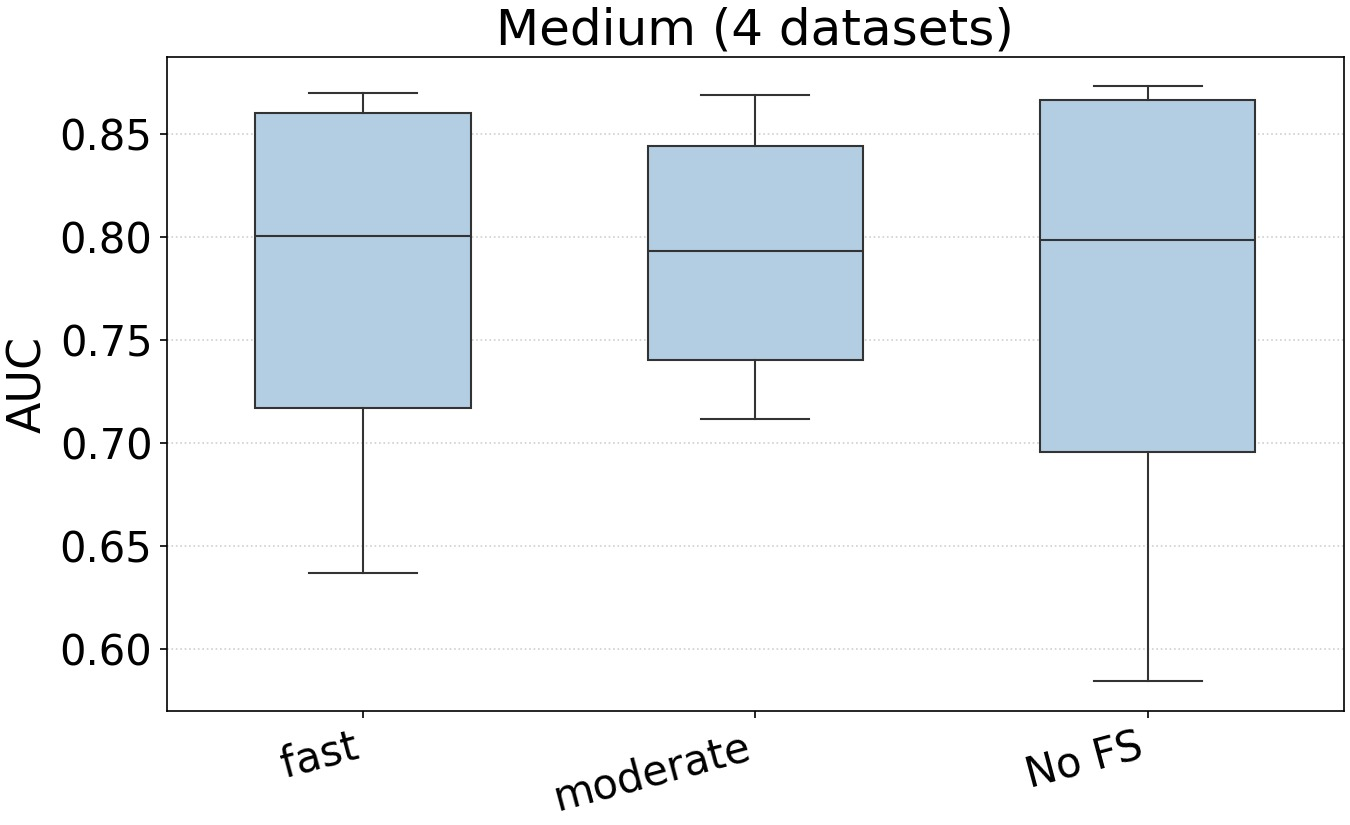
\includegraphics[width=\linewidth]{assets/Dan_Figs/boxplotubset-rem_datasets_fast_moderate_best_FS_rows_Medium_nDatasets-4.jpg}
    \caption{Medium datasets ($n=4$)}
\end{subfigure}
\caption{
Distribution of BEST-mode cross-validated AUC for datasets with only fast and moderate results. Medians for Easy: 0.947 (fast), 0.927 (moderate), 0.936 (No-FS). Medians for Medium: 0.801 (fast), 0.793 (moderate), 0.799 (No-FS). The pattern of comparable or superior performance for fast methods persists across this subset.
}
\label{fig:best_runtime_two_groups}
\end{figure}



\begin{figure}[h!]
\centering
\begin{subfigure}{0.48\linewidth}
    \centering
    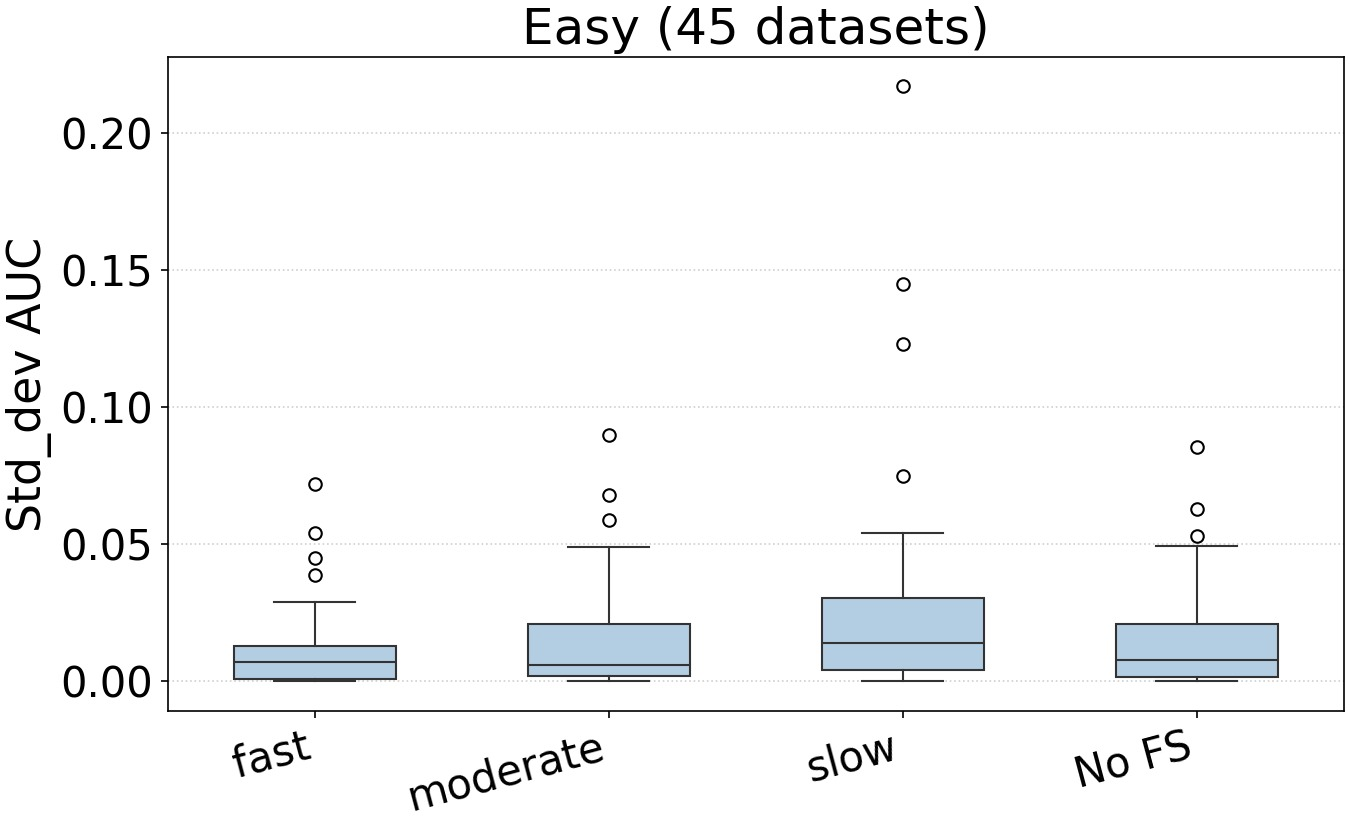
\includegraphics[width=\linewidth]{assets/Dan_Figs/boxplotubset-core_datasets_best_FS_rows_stability_Easy_nDatasets-45.jpg}
    \caption{Easy datasets ($n=45$)}
\end{subfigure}
\hfill
\begin{subfigure}{0.48\linewidth}
    \centering
    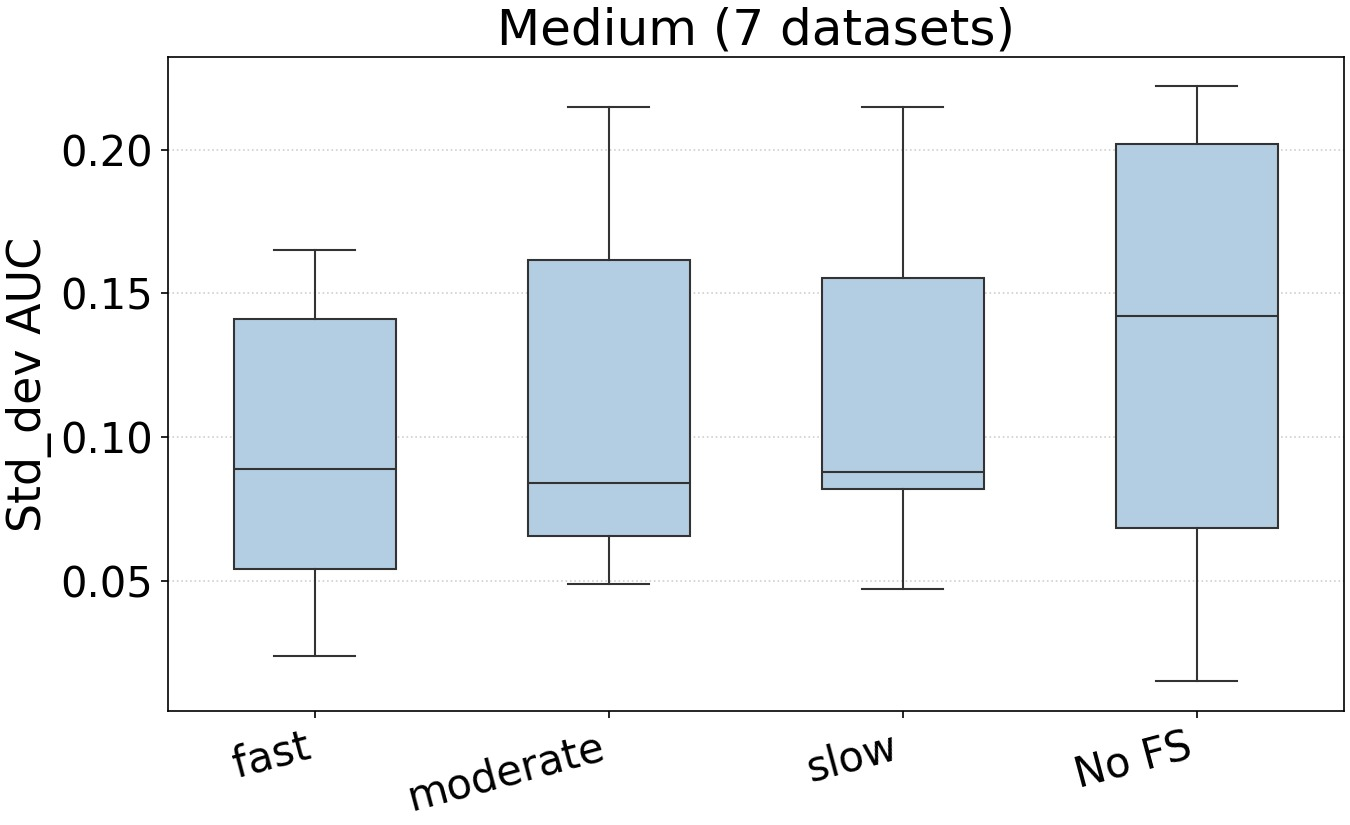
\includegraphics[width=\linewidth]{assets/Dan_Figs/boxplotubset-core_datasets_best_FS_rows_stability_Medium_nDatasets-7.jpg}
    \caption{Medium datasets ($n=7$)}
\end{subfigure}
\caption{
Distribution of BEST-mode cross-validated AUC stability (standard deviation across 5 folds) across runtime buckets and the No-FS baseline. Each point represents the stability of the best FS configuration within each runtime bucket per dataset. Medians for Easy: 0.007 (fast), 0.006 (moderate), 0.014 (slow), 0.008 (No-FS). Medians for Medium: 0.089 (fast), 0.084 (moderate), 0.088 (slow), 0.142 (No-FS). While some visual variation exists, particularly in slow methods, which show higher variability in Easy datasets, fast methods demonstrate consistently low, stable variability.
}
\label{fig:best_runtime_stability}
\end{figure}

We now turn to the BEST-mode analysis (Figures~\ref{fig:best_runtime}--\ref{fig:best_runtime_stability}), where for each dataset and runtime bucket we consider the best-performing configuration. The first key observation is that AUC recovers to the level of the No-FS baseline for both Easy and Medium datasets. This indicates that optimization is indeed worthwhile: the degradation observed in ALL-mode is not inherent to feature selection, but rather a consequence of suboptimal choices of algorithm and hyperparameters.

To evaluate whether higher computational investment yields consistent performance gains, we conduct paired within-dataset comparisons using a one-sided Wilcoxon signed-rank test. For Easy datasets with all three runtime buckets available ($n=43$ paired datasets), the results are 
that fast methods significantly outperform slow methods (median paired difference $-0.009$, meaning fast is 0.009 AUC points higher; win-rate for slow only 2.3\%, Cliffs delta $-0.72$, $p \approx 1.0$ for the hypothesis that slow dominates fast), indicating that increased computational cost actually \emph{degrades} performance. Similarly, moderate methods show no advantage over fast methods (median difference $-0.001$, win-rate for moderate 21\%, Cliffs delta $-0.31$, $p \approx 1.0$). The comparison between moderate and slow shows that moderate also outperforms slow (median difference $-0.003$, win-rate for slow 12\%, Cliffs delta $-0.63$, $p \approx 1.0$).

For the broader Easy subset with at least fast and moderate results, fast methods again show no disadvantage relative to moderate methods (median difference $-0.001$, win-rate for moderate 21\%, Cliffs delta $-0.31$, $p \approx 1.0$).

For Medium datasets, while the sample sizes are smaller and statistical power is limited, the directional pattern is consistent. Among the 7 datasets with all three buckets, fast methods substantially outperform slow ones (median difference $-0.114$, win-rate for slow 0\%, Cliffs delta $-1.0$, $p = 1.0$), and moderate methods also outperform slow ones (median difference $-0.045$, win-rate for slow 0\%, Cliffs delta $-1.0$, $p = 1.0$). Among the Medium datasets with fast and moderate results, fast methods again show an edge (median difference $-0.021$, win-rate for moderate 27\%, Cliffs delta $-0.45$, $p \approx 0.96$).

These paired comparisons provide strong evidence that, even after optimization (BEST-mode), additional computational investment does not yield performance benefits. In fact, fast methods consistently match or exceed the performance of more expensive alternatives. The qualitative pattern in the distributions (Figure~\ref{fig:best_runtime}) reinforces this conclusion: fast methods exhibit tighter distributions with fewer extreme outcomes, particularly for Easy datasets, while achieving comparable or superior median performance.

Taken together, these findings lead to a clear and practical recommendation: \textbf{fast methods provide the best trade-off between computational cost and performance}. This holds for both Easy and Medium datasets. While moderate and slow methods can match performance in some cases after proper optimization, they do not offer a consistent advantage that justifies their additional computational cost, and in many cases actually underperform fast alternatives. 


%%%%%%%%%%%%%%%%%%%%%%%%%%%%%%%%%%%%%%%%%%%%%%%%%%%%%%%%%%%%%%%%%%%
%%% Family Method %%%%%%%%%%%%%%%%%%%%%%%%%%%%%%%%%%%%%%%%%%%%%%%
%%%%%%%%%%%%%%%%%%%%%%%%%%%%%%%%%%%%%%%%%%%%%%%%%%%%%%%%%%%%%%%%%%%

\subsection{Feature Selection Method Family}\label{sec:family_results}

Feature selection methods are commonly grouped into filter, wrapper, hybrid, and ensemble families. Filter methods are computationally efficient and scalable but ignore feature interactions; wrapper methods can achieve higher accuracy but are computationally expensive and prone to overfitting; hybrid methods aim to balance these trade-offs; and ensemble methods often improve robustness through aggregation, although their advantage is data-dependent \cite{theng2025feature,pmc2024hybrid,pmc2023nes,peerj2023review}.

As observed in the runtime analysis, a lack of optimization leads to sub-optimal conclusions. Therefore, to ensure a meaningful comparison across method families and maintain a consistent flow, we restrict the analysis from this point onward to BEST-mode results.

The results in Figure~\ref{fig:fs_family_best} reinforce and refine the insights from the runtime analysis. First, consistent with BEST-mode findings, performance across most method families recovers to the level of the No-FS baseline, indicating that with proper optimization, feature selection does not inherently degrade predictive performance.

To test whether more complex method families consistently outperform simpler ones, we conduct paired within-dataset comparisons using Filter methods as the baseline (the simplest and typically fastest approach). For Easy datasets ($n=48$), the results reveal limited evidence of dominance by higher-cost families. Embedded methods perform comparably to Filter (median paired difference $0$, win-rate 42\%, Cliffs delta $0.04$, $p \approx 0.21$). Ensemble methods show no advantage (median difference $0$, win-rate 38\%, Cliffs delta $-0.06$, $p \approx 0.50$). Wrapper methods show a modest non-significant edge (median difference $-0.0005$, win-rate 19\%, Cliffs delta $-0.31$, $p \approx 1.0$, indicating Filter actually tends to win). 

Importantly, Hybrid methods—often motivated as a sophisticated balance between speed and accuracy—show significantly \emph{worse} performance than Filter methods (median difference $-0.001$, win-rate for Hybrid only 33\%, Cliffs delta $-0.19$, $p \approx 0.99$ for the hypothesis that Hybrid dominates Filter). Neural methods also underperform Filter (median difference $-0.001$, win-rate 27\%, Cliffs delta $-0.24$, $p \approx 0.97$).

For Medium datasets ($n=15$ paired), the pattern is similar but with limited statistical power. Hybrid methods again show the weakest performance relative to Filter (median difference $-0.025$, win-rate for Hybrid 0\%, Cliffs delta $-1.0$, $p = 1.0$). Wrapper methods also underperform Filter (median difference $-0.005$, win-rate 27\%, Cliffs delta $-0.36$, $p \approx 0.90$). Embedded methods show a slight non-significant disadvantage (median difference $-0.004$, win-rate 36\%, Cliffs delta $-0.27$, $p \approx 0.79$). Other families show no significant differences from Filter. 

These findings align with the broader literature showing that hybrid and complex methods do not universally outperform simpler alternatives \cite{nature2024covid,diva2012hybrid,wiley2022hfia,pmc2024hybrid}. The observation is also consistent with the runtime-based conclusions: Filter and Embedded methods are typically among the fastest approaches, while Wrapper and Hybrid methods are more computationally intensive due to their reliance on model-based subset evaluation. The fact that simpler, faster families (particularly Filter) achieve performance comparable to or better than more expensive methods reinforces the earlier recommendation: \textbf{increased computational and methodological complexity does not necessarily translate into improved performance}.

\begin{figure}[h!]
\centering
\begin{subfigure}{0.48\linewidth}
    \centering
    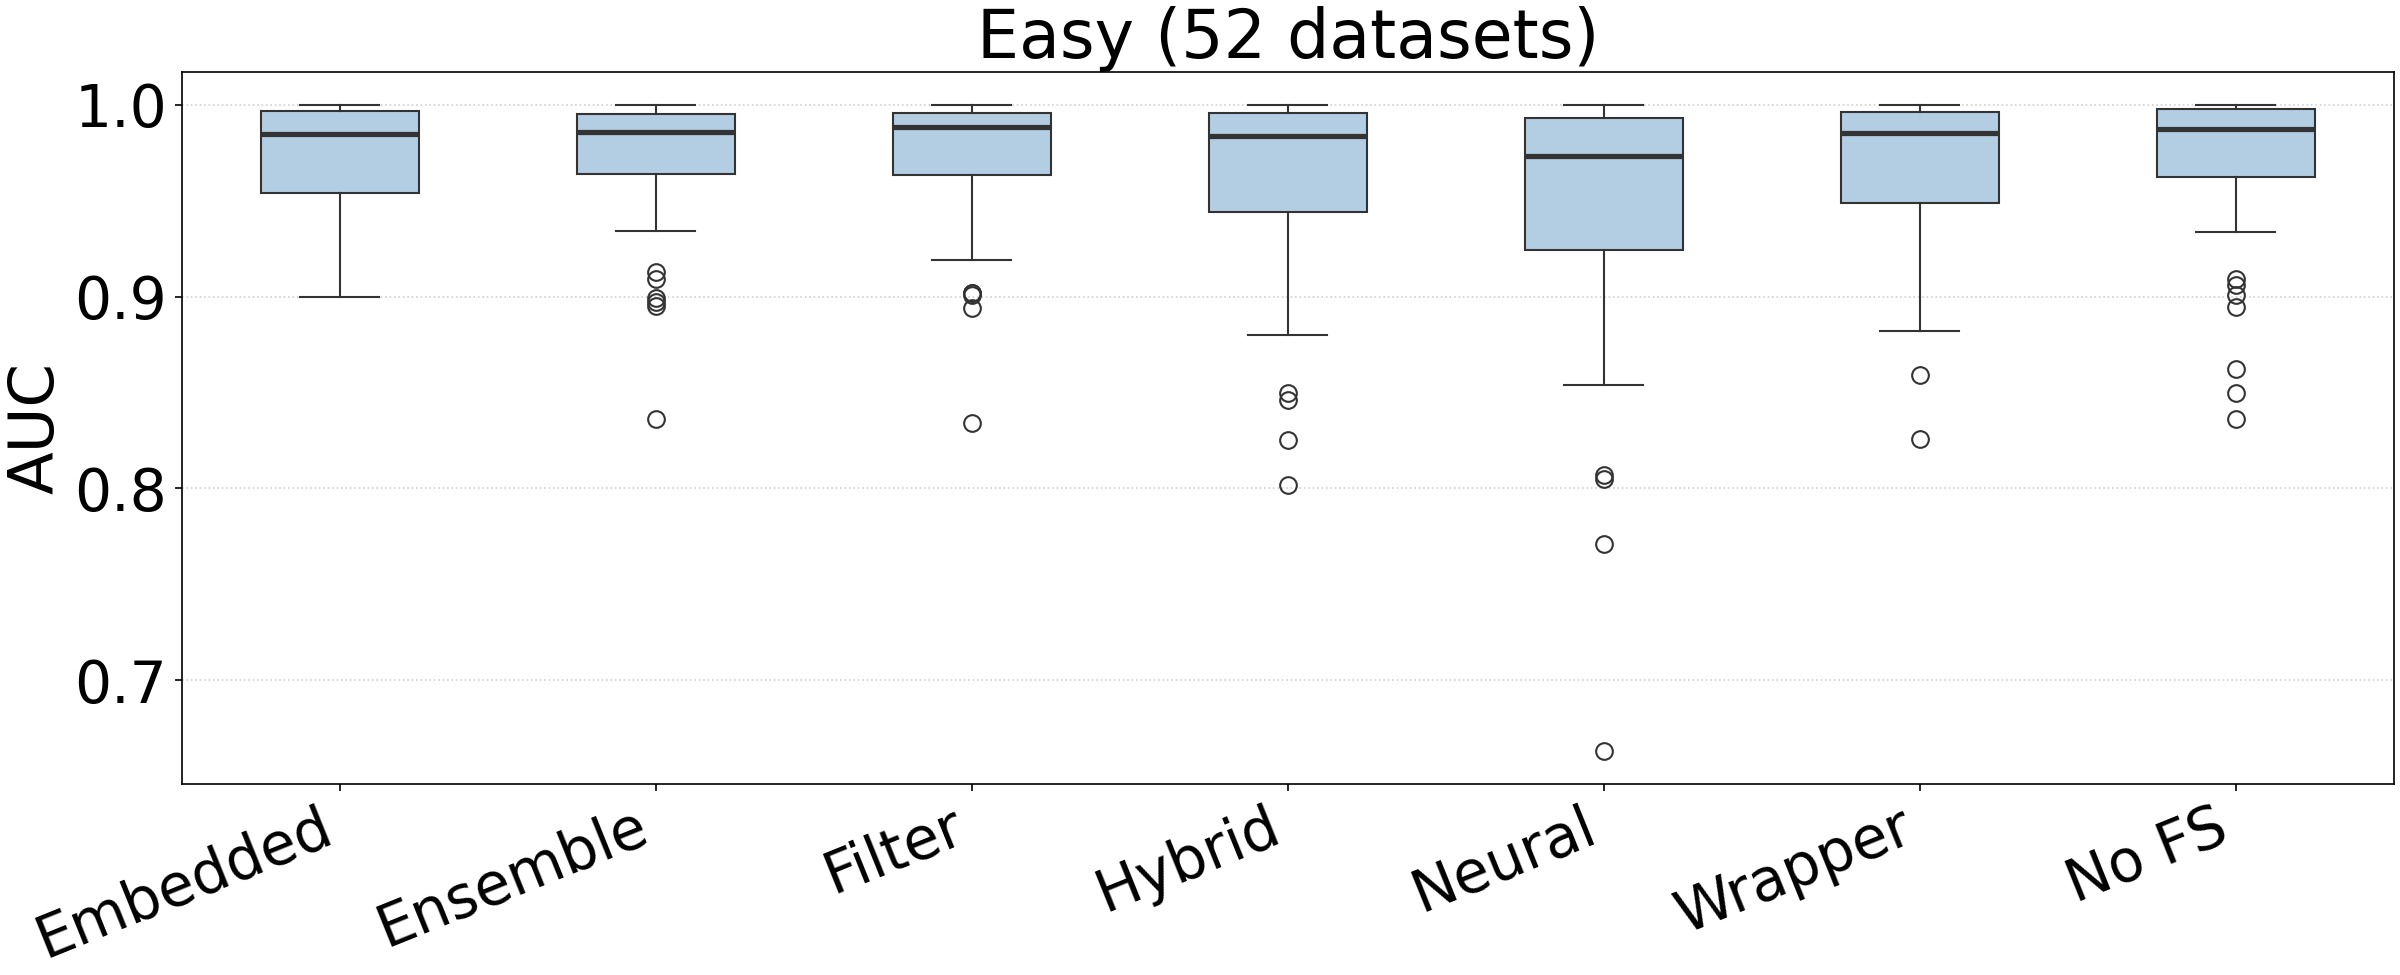
\includegraphics[width=\linewidth]{assets/Dan_Figs/boxplotubset-fs_family_best_FS_rows_mean_AUC_Easy_nDatasets-52.jpg}
    \caption{Easy datasets ($n=48$)}
\end{subfigure}
\hfill
\begin{subfigure}{0.48\linewidth}
    \centering
    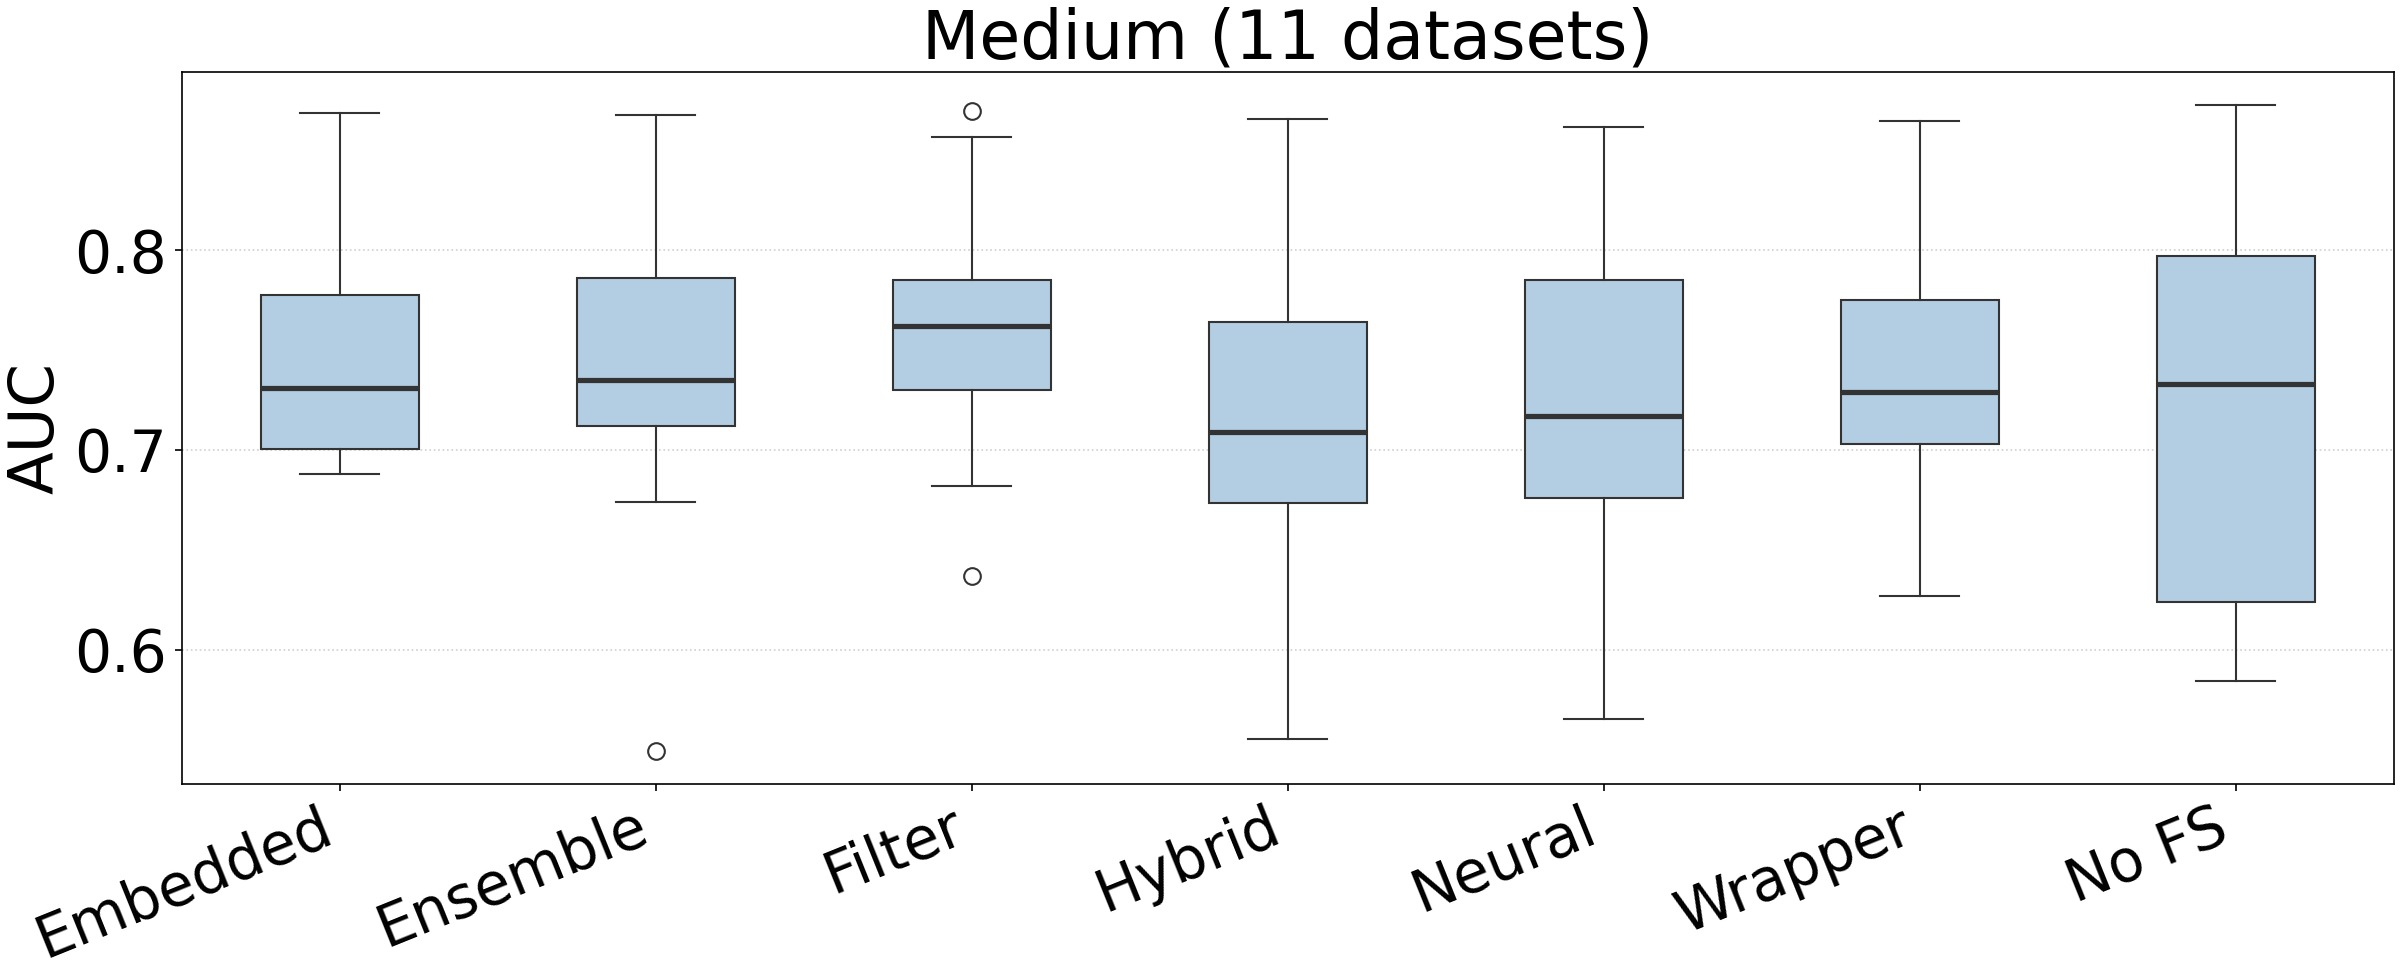
\includegraphics[width=\linewidth]{assets/Dan_Figs/boxplotubset-fs_family_best_FS_rows_mean_AUC_Medium_nDatasets-11.jpg}
    \caption{Medium datasets ($n=15$)}
\end{subfigure}
\caption{
Distribution of BEST-mode cross-validated AUC across feature selection method families and the No-FS baseline. Each point corresponds to a single dataset and represents the best-performing configuration within each method family (one datapoint per dataset $\times$ family). Medians for Easy: 0.9845 (Embedded), 0.9855 (Ensemble), 0.9885 (Filter), 0.9835 (Hybrid), 0.973 (Neural), 0.985 (Wrapper), 0.987 (No-FS). Medians for Medium: 0.731 (Embedded), 0.735 (Ensemble), 0.762 (Filter), 0.709 (Hybrid), 0.717 (Neural), 0.729 (Wrapper), 0.733 (No-FS). Paired within-dataset comparisons using Filter as baseline within the Easy split show that no family significantly dominates Filter. Hybrid methods are significantly dominated by Filter (median difference $-0.001$, Cliffs delta $-0.19$, $p \approx 0.99$). For the Medium split, Hybrid is also dominated by Filter (median difference $-0.025$, Cliffs delta $-1.0$, $p = 1.0$).
}
\label{fig:fs_family_best}
\end{figure}

\vspace{2mm}

The variability analysis (Figure~\ref{fig:fs_family_stability}) complements the performance results. For Easy datasets ($n=48$), all families exhibit relatively low and comparable variability (medians ranging from 0.008 to 0.0145). Paired comparisons using Filter as baseline reveal no significant differences: Embedded (median difference $0$, $p \approx 0.74$), Ensemble (median difference $0$, $p \approx 0.62$), Wrapper (median difference $0$, $p \approx 0.93$), Hybrid (median difference $+0.0025$, $p \approx 0.40$), and Neural (median difference $+0.005$, $p \approx 0.06$) all show comparable stability. The slight tendency for Neural methods to exhibit higher variability does not reach statistical significance.

For Medium datasets ($n=15$ paired), variability is generally higher across all families (medians ranging from 0.065 to 0.089), with the No-FS baseline showing the highest median (0.0855). Paired comparisons again reveal no significant differences from Filter: Embedded (median difference $0$, $p \approx 0.87$), Ensemble (median difference $-0.001$, $p \approx 0.85$), Wrapper (median difference $+0.012$, $p \approx 0.61$), Hybrid (median difference $-0.008$, $p \approx 1.0$), and Neural (median difference $+0.014$, $p \approx 0.44$). The absence of statistical significance reflects both the limited sample size and the genuine similarity in stability across method families.

\begin{figure}[h!]
\centering
\begin{subfigure}{0.48\linewidth}
    \centering
    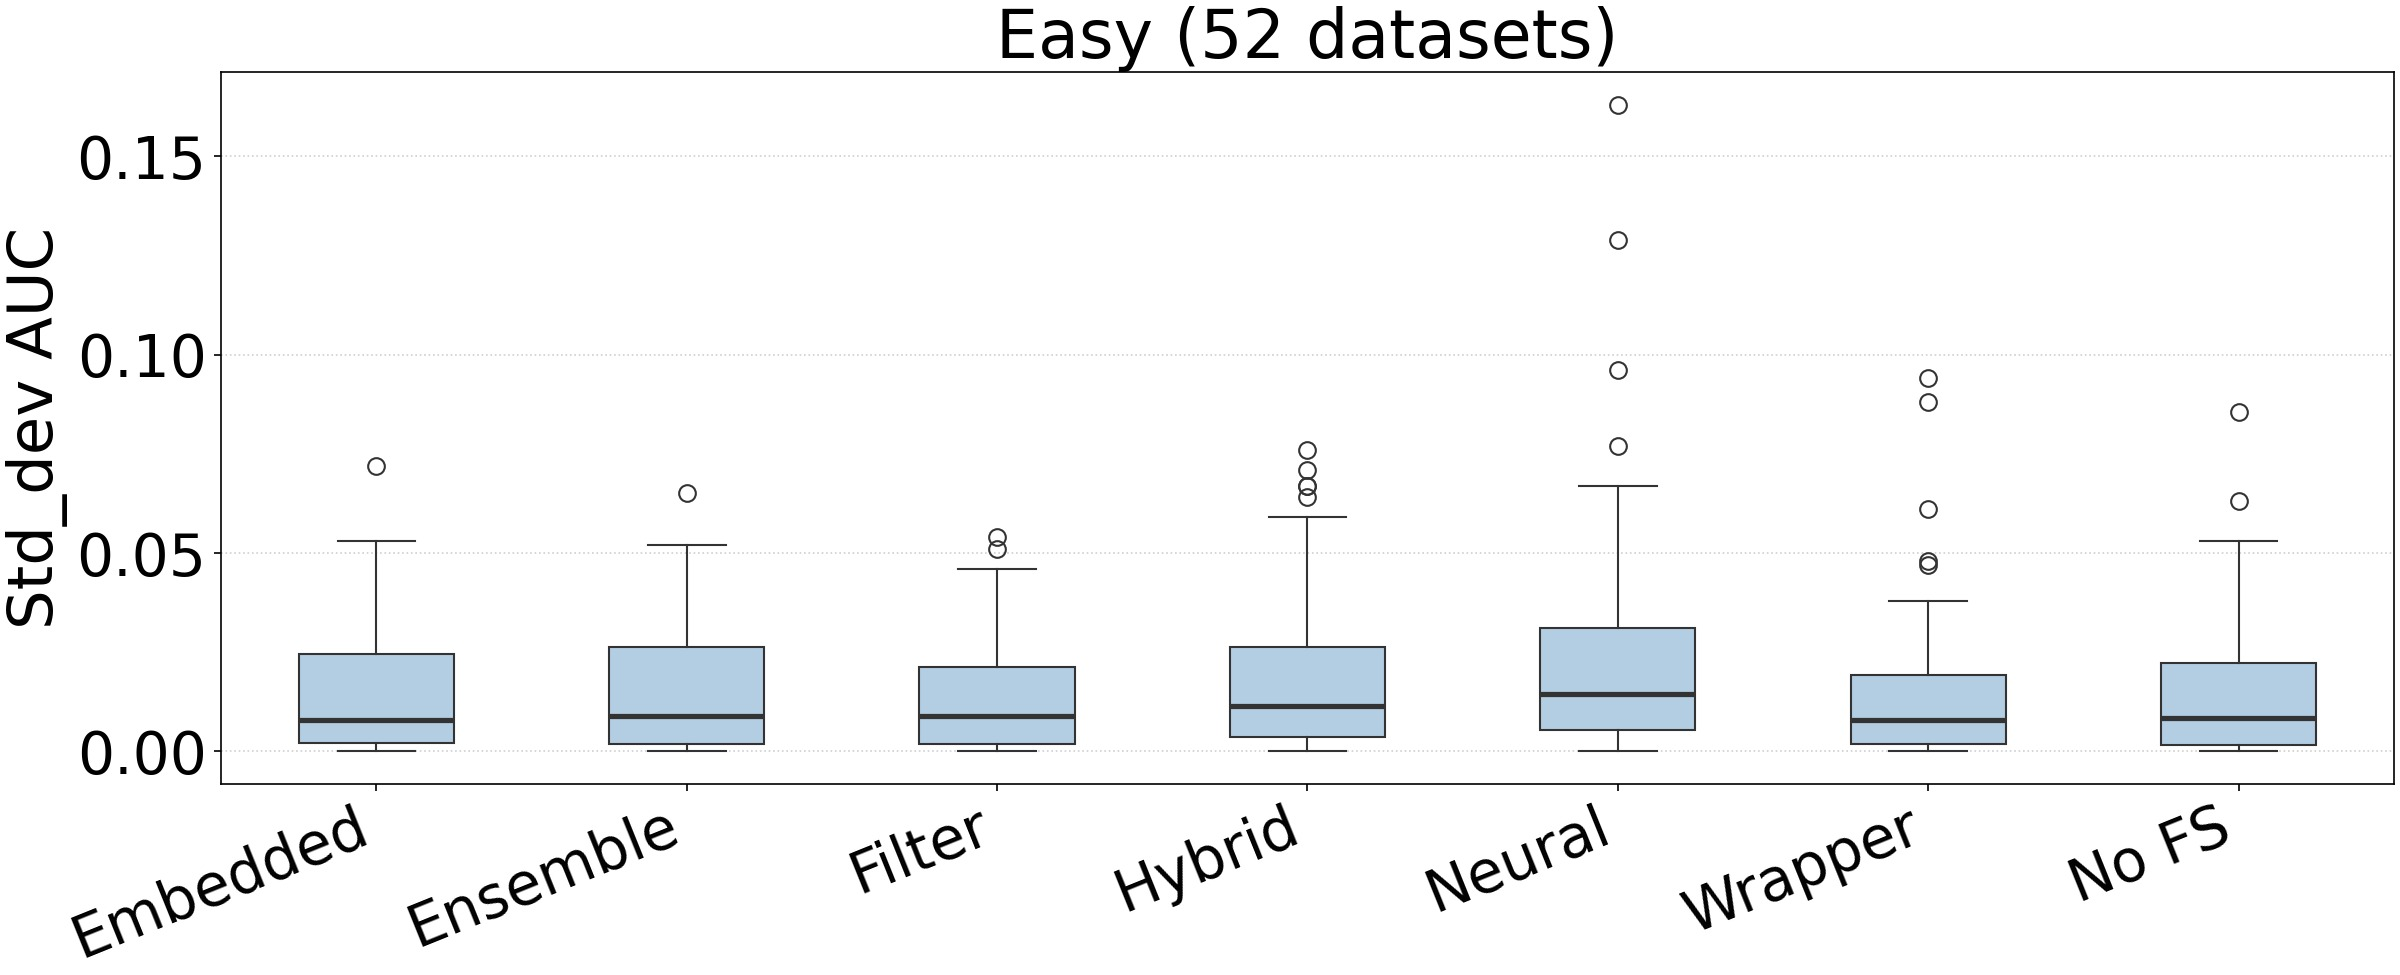
\includegraphics[width=\linewidth]{assets/Dan_Figs/boxplotubset-fs_family_best_FS_rows_stability_StdDevAUC_Easy_nDatasets-52.jpg}
    \caption{Easy datasets ($n=48$)}
\end{subfigure}
\hfill
\begin{subfigure}{0.48\linewidth}
    \centering
    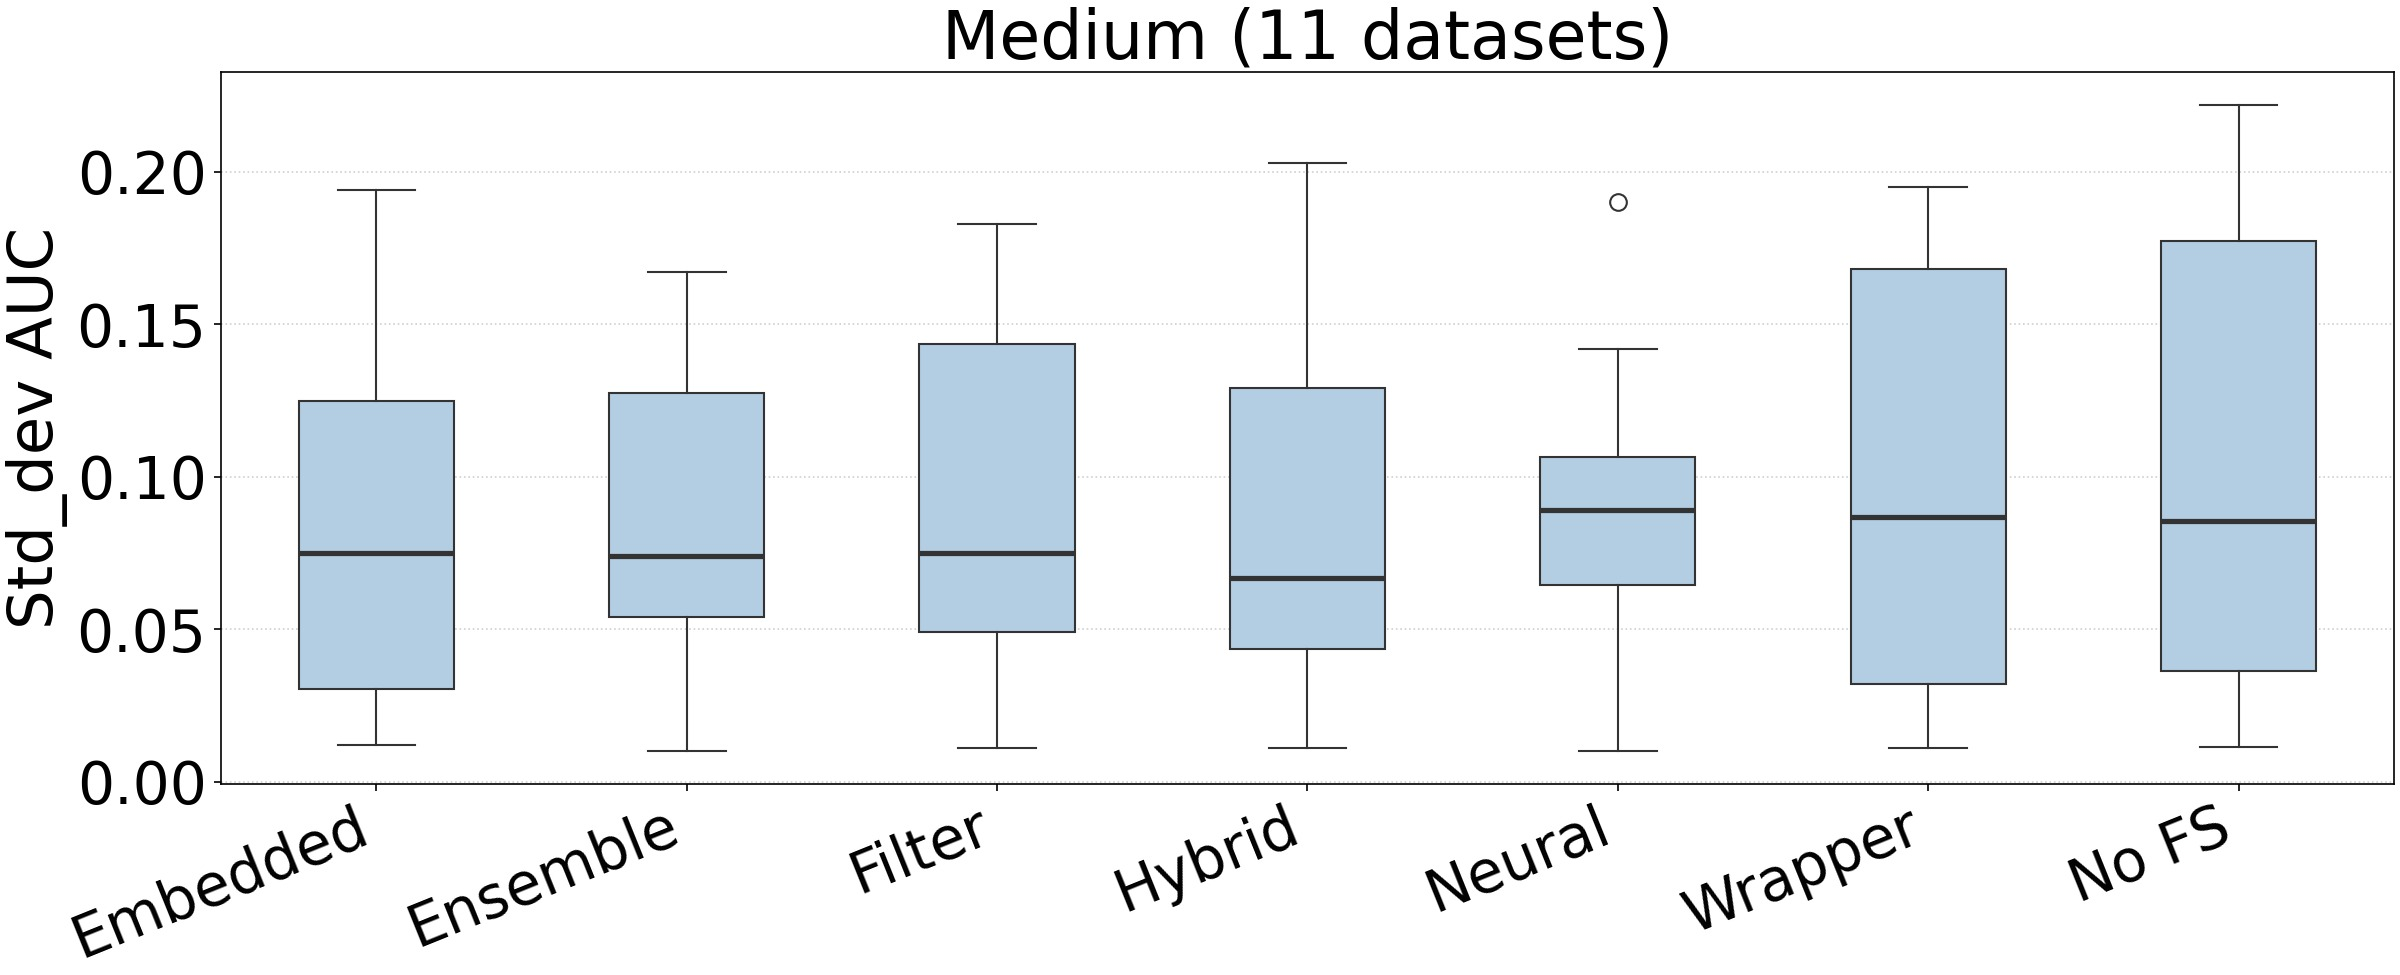
\includegraphics[width=\linewidth]{assets/Dan_Figs/boxplotubset-fs_family_best_FS_rows_stability_StdDevAUC_Medium_nDatasets-11.jpg}
    \caption{Medium datasets ($n=15$)}
\end{subfigure}
\caption{
Distribution of BEST-mode cross-validated AUC stability (standard deviation across 5 folds) across feature selection method families and the No-FS baseline. Medians for Easy: 0.008 (Embedded), 0.009 (Ensemble), 0.009 (Filter), 0.0115 (Hybrid), 0.0145 (Neural), 0.008 (Wrapper), 0.0085 (No-FS). Medians for Medium: 0.075 (Embedded), 0.074 (Ensemble), 0.075 (Filter), 0.067 (Hybrid), 0.089 (Neural), 0.087 (Wrapper), 0.0855 (No-FS). Paired within-dataset comparisons using Filter as baseline reveal no significant differences in stability for either Easy or Medium datasets, indicating that method family does not substantially impact cross-validation reliability.
}
\label{fig:fs_family_stability}
\end{figure}

Taken together, both performance and stability analyses point to the same practical guideline: \textbf{prefer simpler, faster feature selection approaches (particularly Filter methods)}, as they offer a strong trade-off between efficiency, predictive performance, and reliability. More complex families such as Hybrid and Neural methods do not provide consistent advantages and in some cases underperform simpler alternatives.


%%%%%%%%%%%%%%%%%%%%%%%%%%%%%%%%%%%%%%%%%%%%%%%%%%%%%%%%%%%%%%%%%%%
%%% Supervision %%%%%%%%%%%%%%%%%%%%%%%%%%%%%%%%%%%%%%%%%%%%%%%
%%%%%%%%%%%%%%%%%%%%%%%%%%%%%%%%%%%%%%%%%%%%%%%%%%%%%%%%%%%%%%%%%%%


\subsection{Supervision}\label{sec:supervision_results}

We now examine the role of supervision in feature selection. Supervised methods leverage label information during feature selection, while unsupervised methods rely solely on the data structure. Conventional wisdom suggests that supervised methods should consistently outperform unsupervised alternatives, particularly when labels are informative. We test this assumption through paired within-dataset comparisons.

The results, shown in Figure~\ref{fig:fs_supervision_best}, reveal a nuanced pattern that depends critically on dataset difficulty. For Easy datasets ($n=48$ paired datasets), supervised methods show a statistically significant advantage over unsupervised ones (median paired difference $+0.0085$, win-rate 82\%, Cliffs delta $0.80$, $p \approx 2.9 \times 10^{-8}$), indicating that supervision improves accuracy when tasks are well-structured. However, the absolute magnitude of the gain is modest—medians are 0.990 vs.\ 0.9755—and performance is already near saturation for both approaches. Thus, while the advantage is statistically robust and consistent across datasets, its practical value is limited when baseline performance is already excellent.

In contrast, for Medium datasets ($n=15$ paired), the effect of supervision largely disappears. Supervised methods show only a slight and non-significant edge (median difference $+0.010$, win-rate 82\%, Cliffs delta $0.64$, $p \approx 0.028$), with medians of 0.768 vs.\ 0.758. While the win-rate remains high, the effect does not reach strong statistical significance at conventional thresholds, and the absolute difference is small. This suggests that, in more challenging settings where labels may be noisier or less informative relative to intrinsic data structure, supervision does not translate into consistent performance gains. This finding aligns with prior work showing that unsupervised feature selection can be competitive when labels are limited or when the data has strong intrinsic structure \cite{scitepress2019compare}.

\begin{figure}[t]
\centering
\begin{subfigure}[t]{0.48\linewidth}
    \centering
    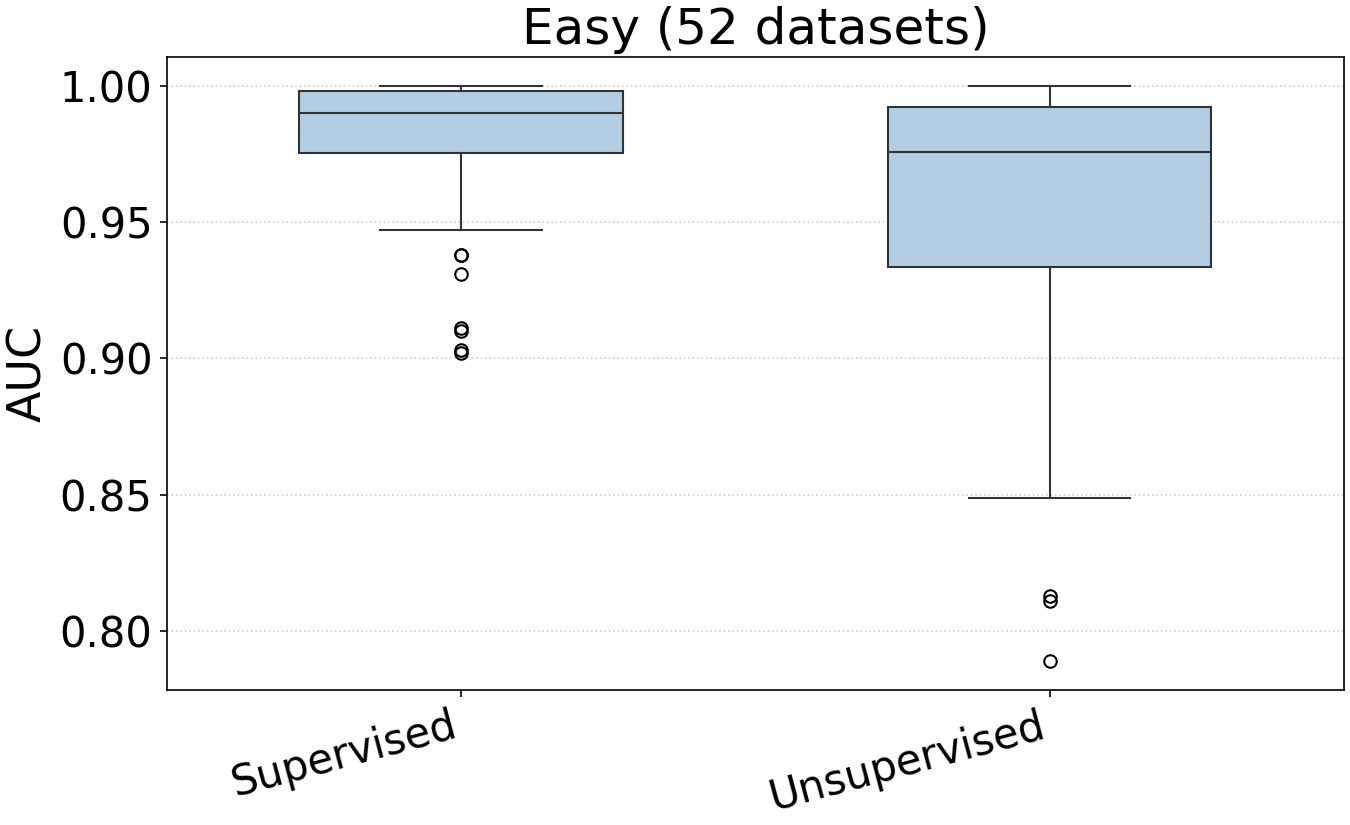
\includegraphics[width=\linewidth]{assets/Dan_Figs/boxplotubset-fs_supervision_best_FS_rows_mean_AUC_Easy_nDatasets-52.jpg}
    \caption{Easy datasets ($n=48$)}
\end{subfigure}
\hfill
\begin{subfigure}[t]{0.48\linewidth}
    \centering
    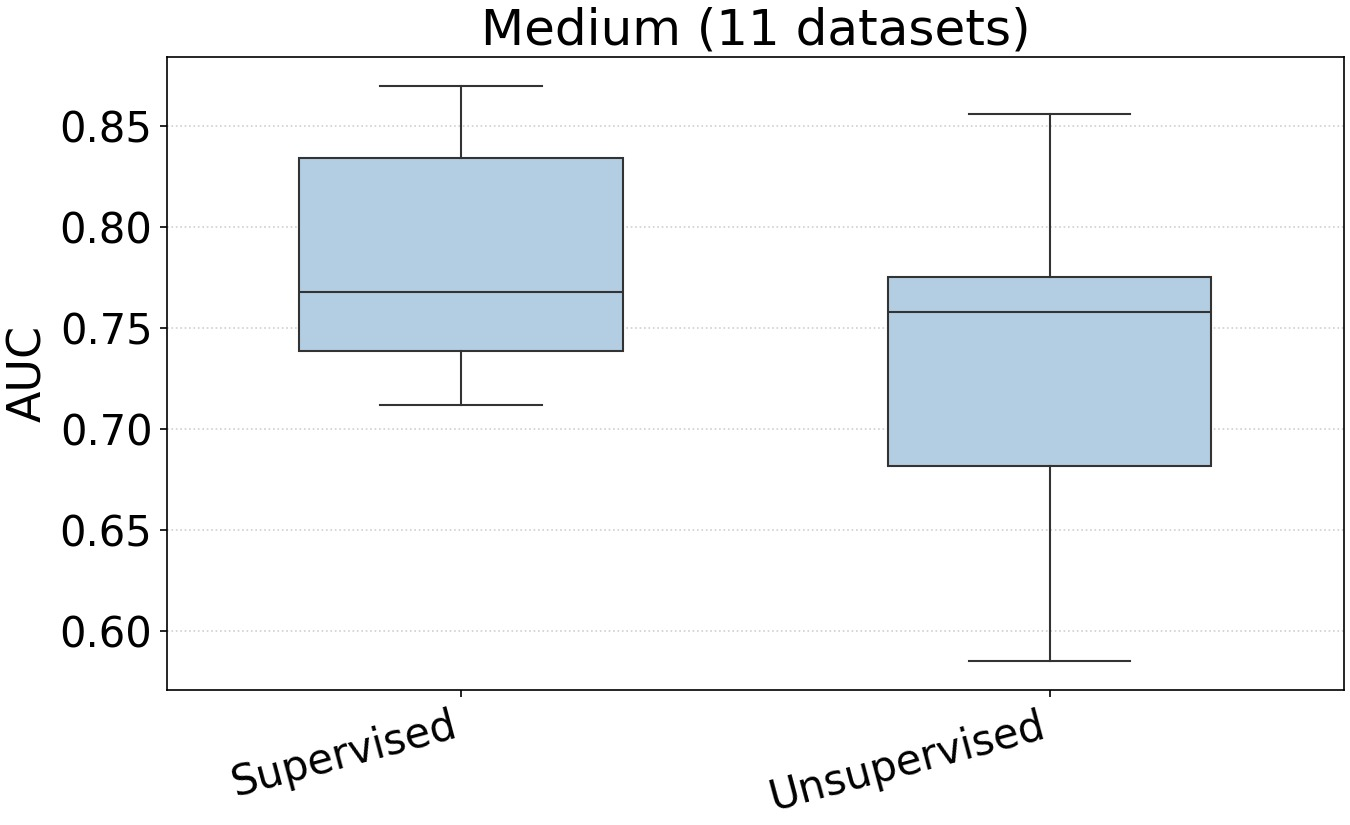
\includegraphics[width=\linewidth]{assets/Dan_Figs/boxplotubset-fs_supervision_best_FS_rows_mean_AUC_Medium_nDatasets-11.jpg}
    \caption{Medium datasets ($n=15$)}
\end{subfigure}
\caption{
Comparison of supervised and unsupervised FS methods using BEST-mode mean 5-fold cross-validation AUC. Medians for Easy: 0.990 (Supervised), 0.9755 (Unsupervised). Medians for Medium: 0.768 (Supervised), 0.758 (Unsupervised). Paired within-dataset tests: For Easy ($n=48$), supervised methods significantly outperform unsupervised ones (median difference $+0.0085$, win-rate 82\%, Cliffs delta $0.80$, $p \approx 2.9 \times 10^{-8}$). For Medium ($n=15$), the advantage is modest and marginally significant (median difference $+0.010$, win-rate 82\%, Cliffs delta $0.64$, $p \approx 0.028$), suggesting diminished value of supervision in more challenging settings.
}
\label{fig:fs_supervision_best}
\end{figure}

To provide additional context, we revisit the ALL-mode setting in Figure~\ref{fig:fs_supervision_all}, where neither algorithm choice nor hyperparameters are optimized. In this low-effort regime, supervised methods show a much larger advantage. For Easy datasets, supervised methods substantially outperform unsupervised ones (median 0.926 vs.\ 0.765, $p \ll 10^{-10}$), demonstrating a large and consistent benefit across all configurations. For Medium datasets, the advantage persists but is noticeably smaller (median 0.600 vs.\ 0.555, $p \approx 4.9 \times 10^{-7}$). This indicates that supervision helps substantially when optimization effort is low, but the gap narrows considerably—and in Medium datasets, nearly vanishes—once proper optimization is applied (BEST-mode).

\begin{figure}[t]
\centering
\begin{subfigure}[t]{0.48\linewidth}
    \centering
    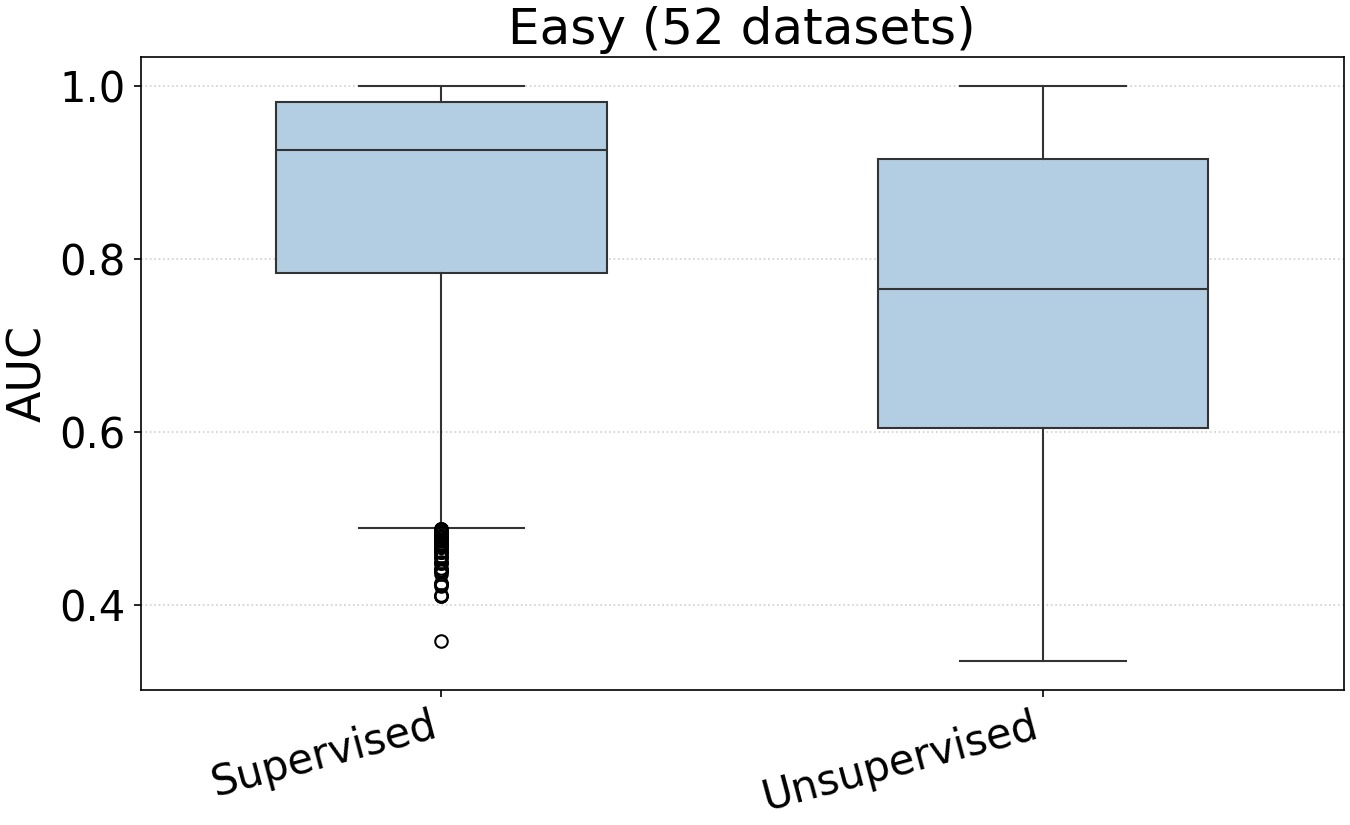
\includegraphics[width=\linewidth]{assets/Dan_Figs/boxplotubset-fs_supervision_all_FS_rows_mean_AUC_Easy_nDatasets-52.jpg}
    \caption{Easy datasets ($n=48$)}
\end{subfigure}
\hfill
\begin{subfigure}[t]{0.48\linewidth}
    \centering
    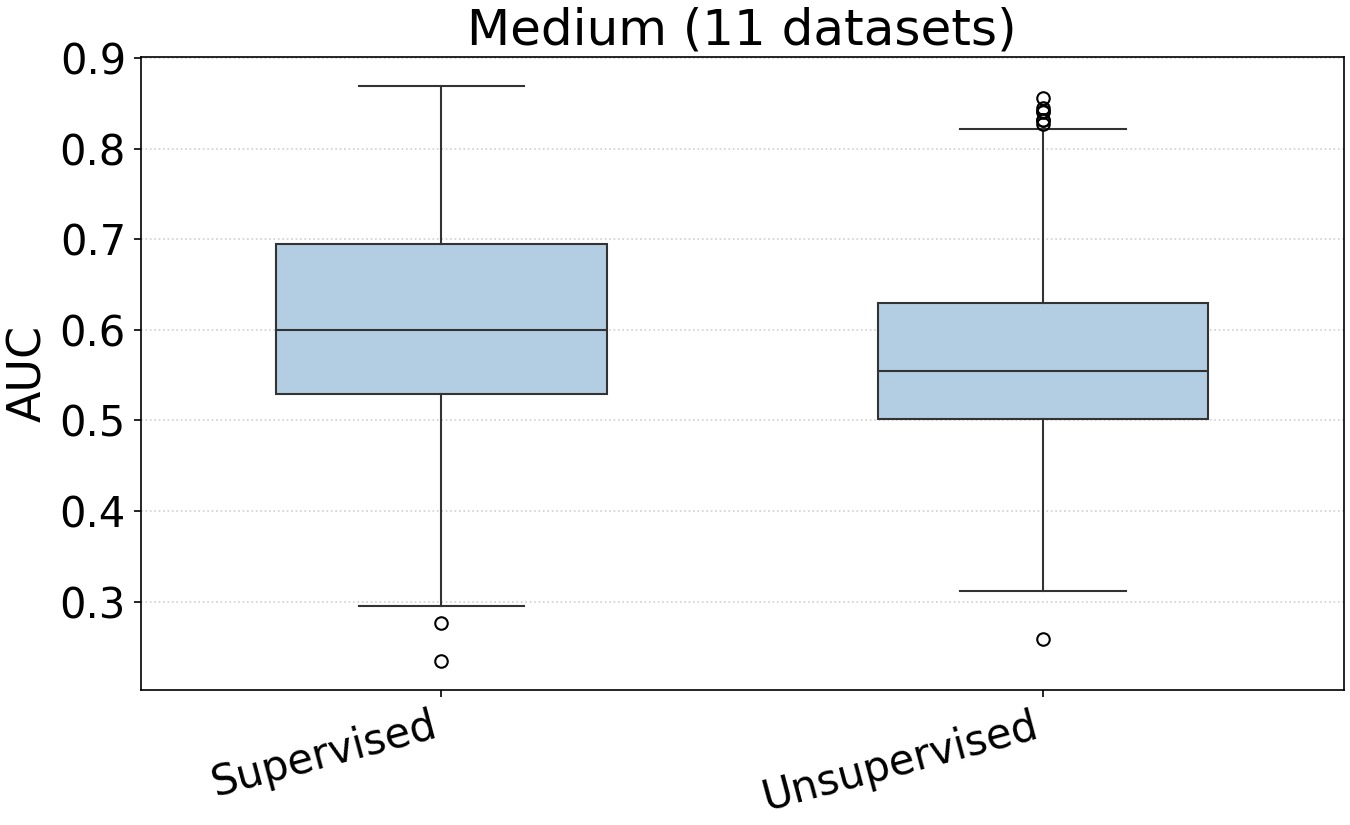
\includegraphics[width=\linewidth]{assets/Dan_Figs/boxplotubset-fs_supervision_all_FS_rows_mean_AUC_Medium_nDatasets-11.jpg}
    \caption{Medium datasets ($n=15$)}
\end{subfigure}
\caption{
Comparison of supervised and unsupervised feature selection across ALL-mode configurations, using mean 5-fold cross-validation AUC. Medians for Easy: 0.926 (Supervised), 0.765 (Unsupervised). Medians for Medium: 0.600 (Supervised), 0.555 (Unsupervised). In the unoptimized setting, supervised methods show substantial advantages (Easy: $p \ll 10^{-10}$; Medium: $p \approx 4.9 \times 10^{-7}$), though the gap is noticeably smaller for Medium datasets. These results demonstrate that supervision provides stronger benefits when optimization is not performed, but this advantage diminishes substantially with proper tuning.
}
\label{fig:fs_supervision_all}
\end{figure}

The stability analysis (Figure~\ref{fig:fs_supervision_stability}) further reinforces these patterns. For Easy datasets ($n=48$ paired), supervised methods exhibit significantly lower variability than unsupervised ones (median paired difference $-0.0055$, meaning supervised has 0.0055 lower standard deviation; medians 0.006 vs.\ 0.0115, $p \approx 0.021$), indicating more stable cross-validation performance. This suggests that, in well-structured problems, supervision not only improves accuracy but also enhances reliability.

For Medium datasets ($n=15$ paired), however, this stability advantage disappears. Supervised and unsupervised methods show comparable variability (median difference $-0.007$, medians 0.051 vs.\ 0.058, $p \approx 0.90$, with the non-significant difference actually favoring supervised slightly in absolute terms but showing no consistent within-dataset pattern). This consistency across both performance and stability metrics reinforces the conclusion that, in more challenging settings, supervision does not translate into meaningful improvements.

\begin{figure}[t]
\centering
\begin{subfigure}[t]{0.48\linewidth}
    \centering
    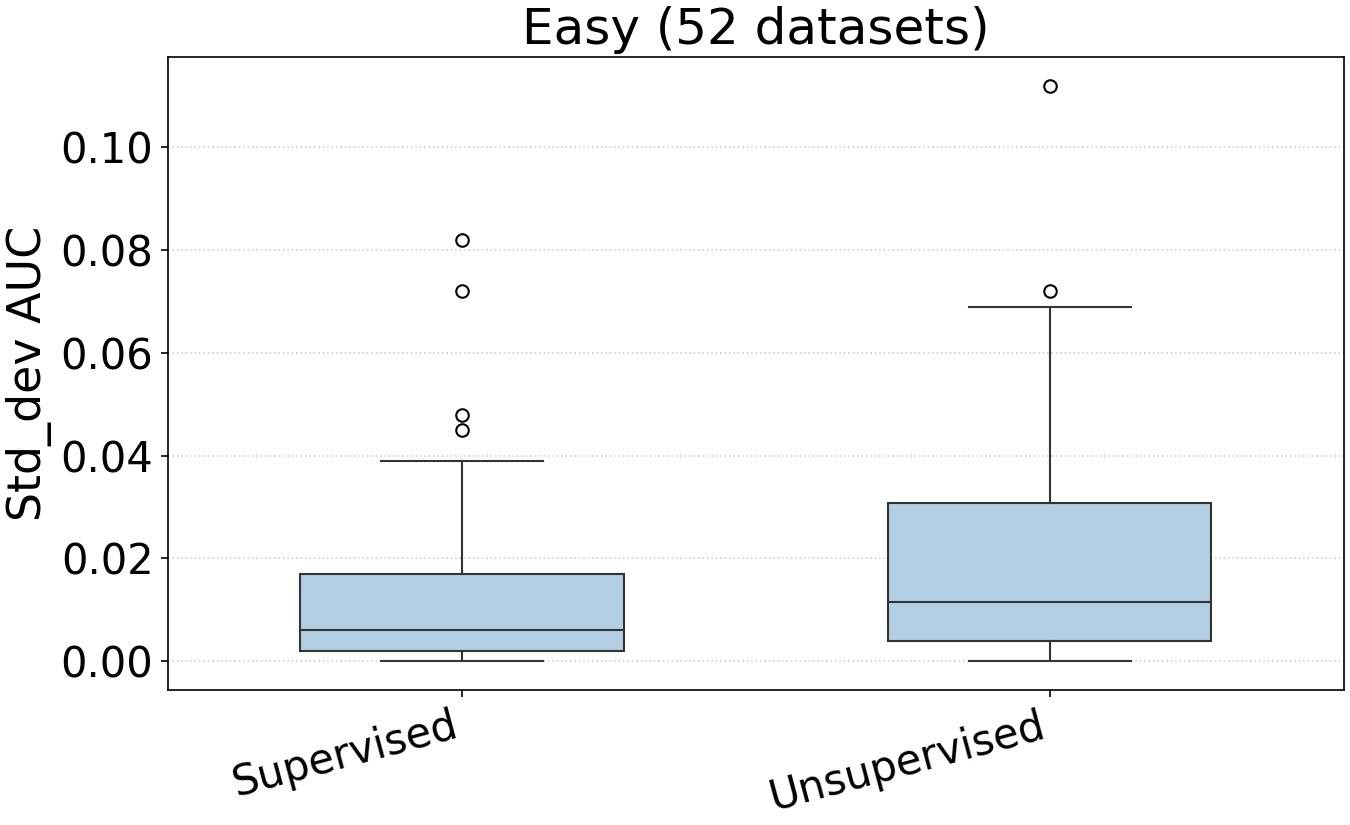
\includegraphics[width=\linewidth]{assets/Dan_Figs/boxplotubset-fs_supervision_best_FS_rows_stability_StdDevAUC_Easy_nDatasets-52.jpg}
    \caption{Easy datasets ($n=48$)}
\end{subfigure}
\hfill
\begin{subfigure}[t]{0.48\linewidth}
    \centering
    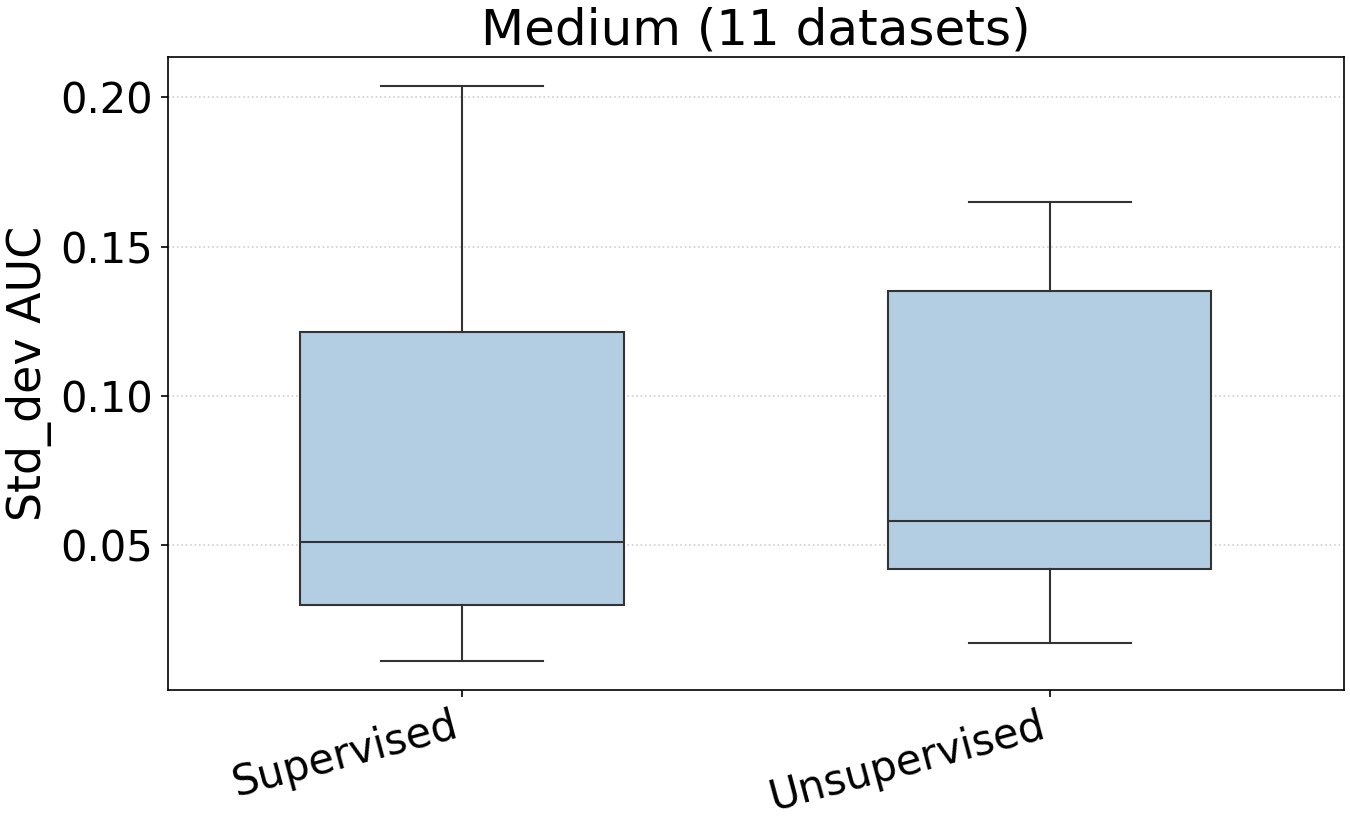
\includegraphics[width=\linewidth]{assets/Dan_Figs/boxplotubset-fs_supervision_best_FS_rows_stability_StdDevAUC_Medium_nDatasets-11.jpg}
    \caption{Medium datasets ($n=15$)}
\end{subfigure}
\caption{
Comparison of supervised and unsupervised feature selection methods in terms of variability (Std$_{\text{dev}}$ AUC from 5-fold CV), using BEST-mode selection. For each dataset and supervision type, the FS configuration with the highest mean CV AUC is selected. Medians for Easy: 0.006 (Supervised), 0.0115 (Unsupervised). Medians for Medium: 0.051 (Supervised), 0.058 (Unsupervised). Paired within-dataset tests: For Easy ($n=48$), supervised methods exhibit significantly lower variability (median difference $-0.0055$, $p \approx 0.021$), indicating more stable performance. For Medium ($n=15$), no significant difference is observed ($p \approx 0.90$), with comparable stability across supervision types.
}
\label{fig:fs_supervision_stability}
\end{figure}

These results highlight an important practical insight regarding supervision. First, note that supervision is largely exogenous: either the data is labeled, or it is not. When the problem is Easy and labels are available, supervision provides statistically significant gains in both accuracy and stability—but these gains are of limited practical value since performance is already near saturation. In contrast, for Medium problems where improvement is most needed, supervision does not lead to consistent gains in either accuracy or stability.

This offers a counterintuitive implication: rather than investing heavily in labeling efforts for challenging datasets, it may be more effective to collect additional unlabeled data and leverage unsupervised feature selection. When unlabeled data is cheap and abundant, as is often the case in modern data pipelines, \textbf{unsupervised methods can offer a more scalable and equally effective alternative}, particularly for datasets that are not easily separable. This challenges the conventional prioritization of labeled data acquisition and suggests that the marginal value of labels for feature selection diminishes as problem difficulty increases.


%%%%%%%%%%%%%%%%%%%%%%%%%%%%%%%%%%%%%%%%%%%%%%%%%%%%%%%%%%%%%%%%%%%
%%% Effort %%%%%%%%%%%%%%%%%%%%%%%%%%%%%%%%%%%%%%%%%%%%%%%
%%%%%%%%%%%%%%%%%%%%%%%%%%%%%%%%%%%%%%%%%%%%%%%%%%%%%%%%%%%%%%%%%%%
\subsection{Implementation Effort: Library vs.\ Research Code}\label{sec:implementation_results}

Beyond supervision, we examine another practical resource: implementation effort. In practice, feature selection (FS) methods can either be readily available through mature libraries or require custom implementation based on research papers. This distinction captures a real-world trade-off between ease of adoption and potential performance gains. Conventional wisdom suggests that cutting-edge research methods, while harder to implement, should outperform mature library implementations. We test this assumption through paired within-dataset comparisons.

Figure~\ref{fig:fs_adoption_best} presents the performance comparison. For Easy datasets, the results are counterintuitive: Library-based methods show a statistically significant advantage over Research Paper implementations (median paired difference $+0.001$, meaning Library methods achieve 0.001 higher AUC; win-rate 58\%, Cliffs delta $0.36$, $p \approx 0.006$). While the absolute difference is small (medians: 0.987 vs.\ 0.990), the consistency of the pattern—with Library methods winning on 58\% of datasets—indicates that readily available library implementations are not only sufficient but often superior to custom research code.

For Medium datasets, the pattern is even stronger. Library methods significantly outperform Research Paper implementations (median difference $+0.015$, win-rate 82\%, Cliffs delta $0.64$, $p \approx 0.016$), with a large effect size. Although the marginal medians suggest Research Paper methods achieve slightly higher values on average (0.747 vs.\ 0.768), the paired comparison reveals that \emph{within the same datasets}, Library methods more consistently win. This discrepancy between marginal and paired comparisons likely reflects differences in which datasets have Library vs.\ Research Paper implementations available, underscoring the value of within-dataset paired testing.

These results challenge the assumption that increased implementation effort yields better performance. Several factors may explain this pattern: (i) library implementations benefit from extensive testing, debugging, and refinement by the community over time, (ii) research code may suffer from implementation errors, incomplete documentation, or suboptimal default settings when adapted from the original study context, (iii) library methods are often better optimized for general use cases and diverse data characteristics, and (iv) reproducibility issues with research code can lead to degraded performance when ported to new environments. In many cases, readily available library methods offer a competitive and far more efficient alternative, especially when considering development time, maintenance burden, and reproducibility.

\begin{figure}[t!]
\centering
\begin{subfigure}[t]{0.48\linewidth}
    \centering
    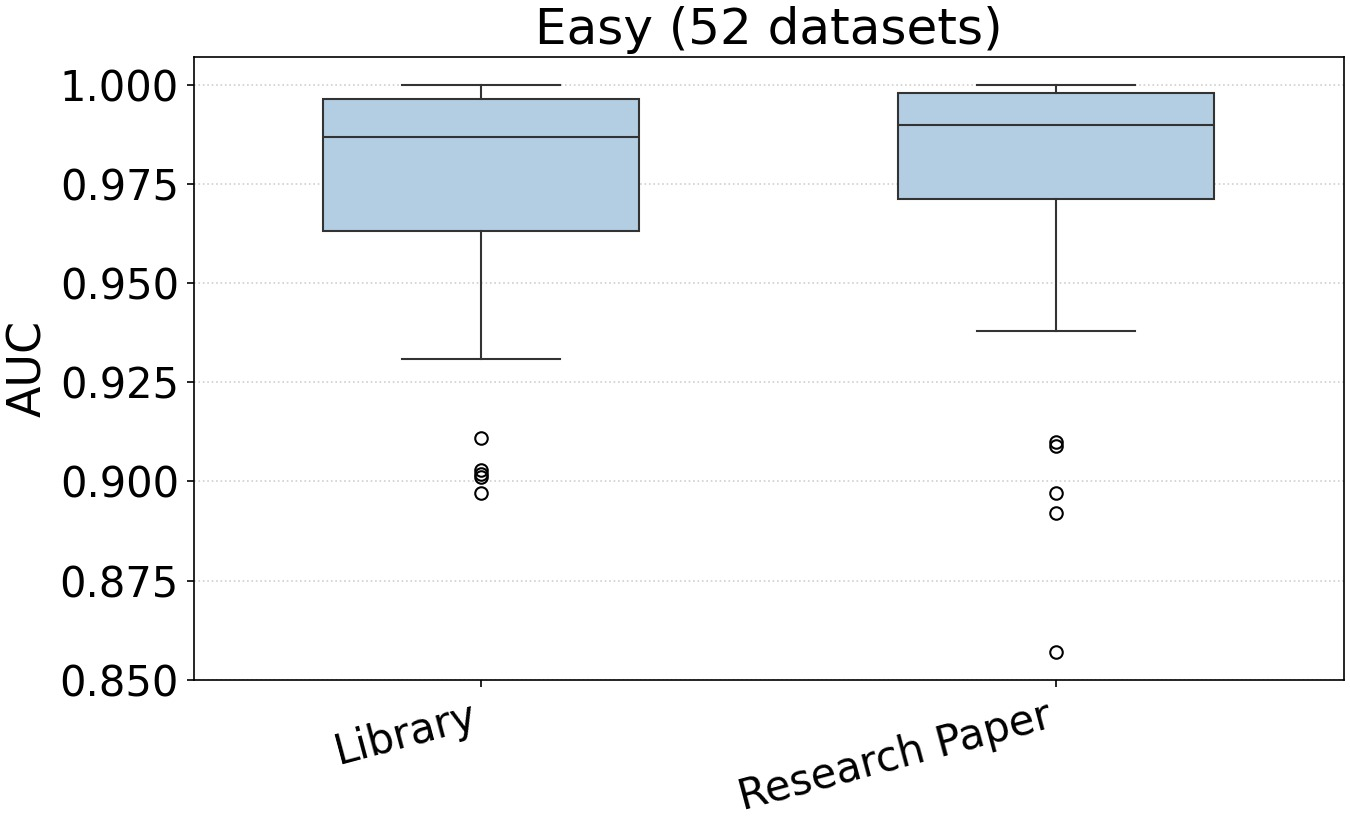
\includegraphics[width=\linewidth]{assets/Dan_Figs/boxplotubset-fs_adoption_best_FS_rows_mean_AUC_Easy_nDatasets-52.jpg}
    \caption{Easy datasets}
\end{subfigure}
\hfill
\begin{subfigure}[t]{0.48\linewidth}
    \centering
    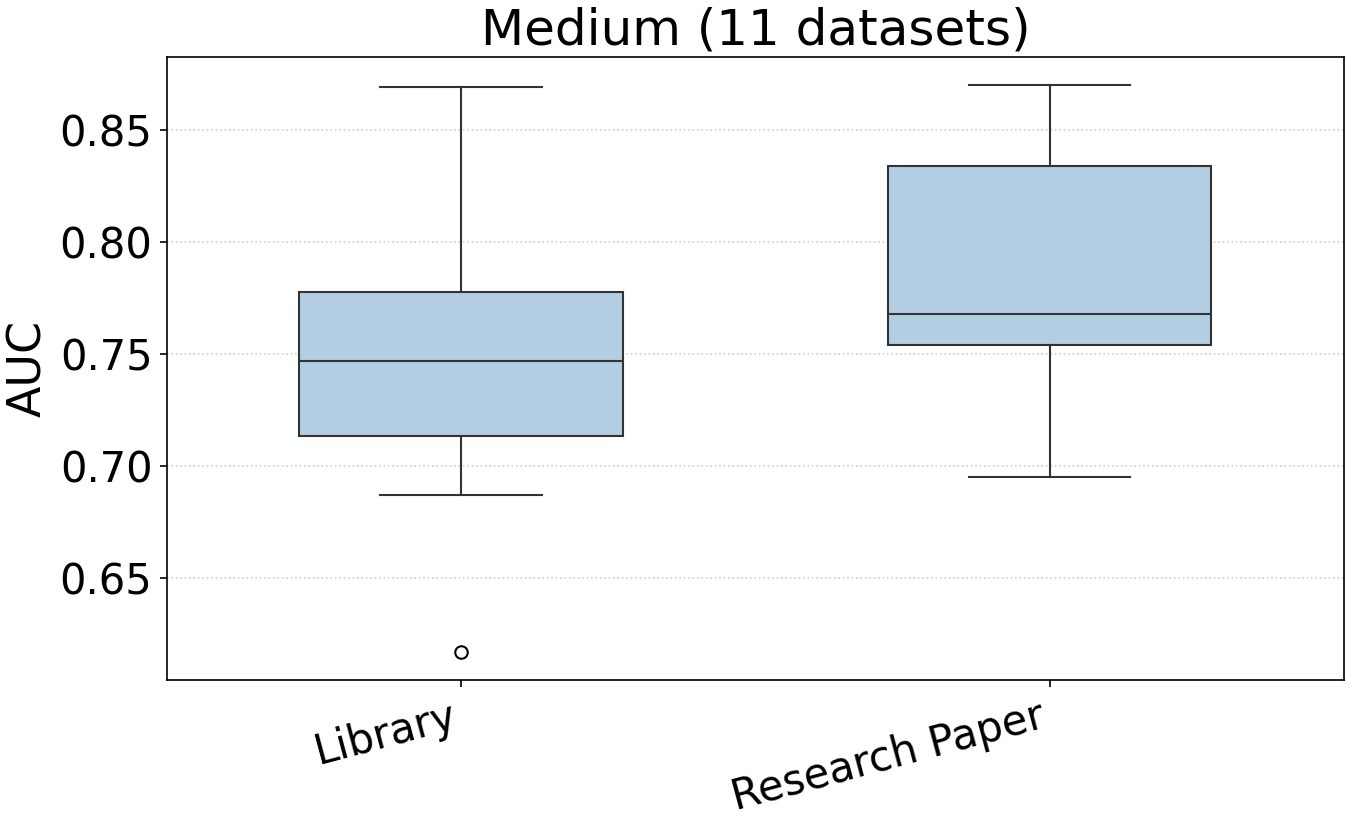
\includegraphics[width=\linewidth]{assets/Dan_Figs/boxplotubset-fs_adoption_best_FS_rows_mean_AUC_Medium_nDatasets-11.jpg}
    \caption{Medium datasets}
\end{subfigure}
\caption{
Comparison of implementation effort in the BEST setting, contrasting library-based feature selection methods with methods taken from research papers. For each dataset and adoption type, we keep the feature-selection run with the highest mean 5-fold cross-validation AUC. Medians for Easy: 0.987 (Library), 0.990 (Research Paper). Medians for Medium: 0.747 (Library), 0.768 (Research Paper). Paired within-dataset comparisons reveal that Library methods significantly outperform Research Paper implementations in both Easy datasets (median difference $+0.001$, win-rate 58\%, Cliffs delta $0.36$, $p \approx 0.006$) and Medium datasets (median difference $+0.015$, win-rate 82\%, Cliffs delta $0.64$, $p \approx 0.016$), suggesting that additional implementation effort does not translate into consistent performance advantages and may actually degrade performance.
}
\label{fig:fs_adoption_best}
\end{figure}

We further examine whether implementation effort affects stability. Figure~\ref{fig:fs_adoption_stability} shows the variability (Std.\ dev AUC) across folds. For Easy datasets, Library and Research Paper methods exhibit comparable stability (medians 0.008 vs.\ 0.006), with no statistically significant within-dataset difference (median paired difference $+0.002$, $p \approx 0.31$). The slightly lower median for Research Paper methods in absolute terms does not reflect consistent within-dataset superiority—the paired test shows no systematic pattern.

Similarly, for Medium datasets, variability remains comparable between the two approaches (medians 0.069 vs.\ 0.061, median paired difference $+0.008$, $p \approx 0.69$), with no consistent advantage for either side. The absence of significant differences indicates that implementation source does not substantially impact cross-validation reliability.

\begin{figure}[t!]
    \centering
    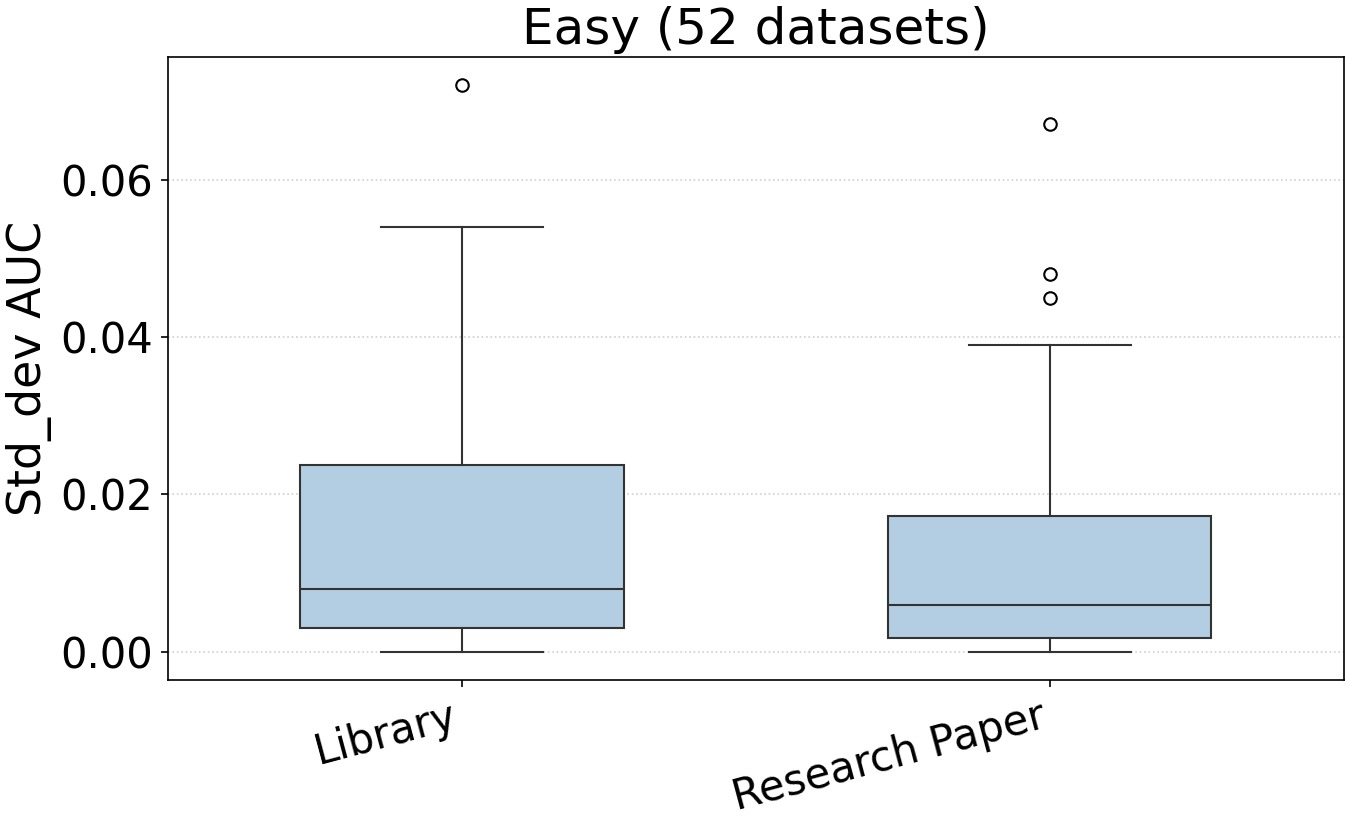
\includegraphics[width=0.48\linewidth]{assets/Dan_Figs/boxplotubset-fs_adoption_best_FS_rows_stability_StdDevAUC_Easy_nDatasets-52.jpg}
    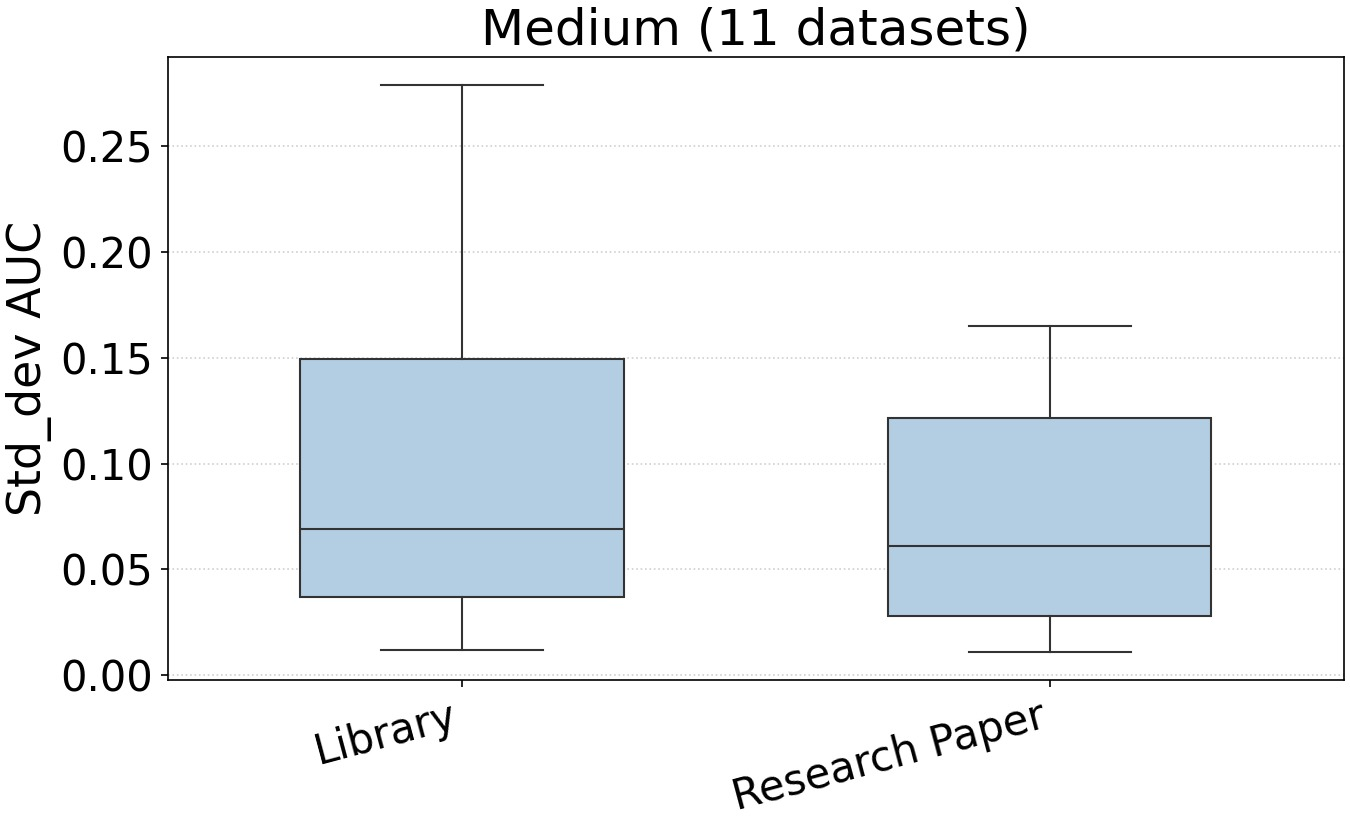
\includegraphics[width=0.48\linewidth]{assets/Dan_Figs/boxplotubset-fs_adoption_best_FS_rows_stability_StdDevAUC_Medium_nDatasets-11.jpg}
   \caption{Stability comparison (Std.\ dev AUC) between library-based and research-paper-based feature selection implementations. Results are shown for Easy datasets (left) and Medium datasets (right), where each point represents the stability metric for the best-performing FS configuration within each adoption type per dataset. Medians for Easy: 0.008 (Library), 0.006 (Research Paper). Medians for Medium: 0.069 (Library), 0.061 (Research Paper). Paired within-dataset comparisons show no significant differences in stability (Easy: median difference $+0.002$, $p \approx 0.31$; Medium: median difference $+0.008$, $p \approx 0.69$), indicating comparable reliability between library-based and research-code implementations despite the performance advantage of library methods.}
    \label{fig:fs_adoption_stability}
\end{figure}

Both accuracy and stability results indicate that library-based methods provide comparable or superior performance to research-code implementations without the associated development costs. This pattern likely reflects differences in software engineering practices: library implementations benefit from extensive testing, community review, and iterative refinement, whereas research code may suffer from implementation errors or suboptimal adaptation to new contexts. These findings suggest that practitioners should default to established library implementations (e.g., scikit-learn, scikit-feature) unless specific evidence indicates benefits from custom code for their application domain. The performance advantage of library methods aligns with the broader pattern observed across resource dimensions, where lower-cost alternatives frequently match or exceed higher-cost alternatives.


%%%%%%%%%%%%%%%%%%%%%%%%%%%%%%%%%%%%%%%%%%%%%%%%%%%%%%%%%%%%%%%%%%%
%%% Multiclass %%%%%%%%%%%%%%%%%%%%%%%%%%%%%%%%%%%%%%%%%%%%%%%
%%%%%%%%%%%%%%%%%%%%%%%%%%%%%%%%%%%%%%%%%%%%%%%%%%%%%%%%%%%%%%%%%%%

\subsection{Multiclass and Nearly-Balanced Datasets}\label{sec:multiclass_balanced_results}

To assess the generalizability of our findings beyond the binary classification setting, we replicate the paired dominance analysis on two additional dataset collections: (i) 39 multiclass datasets evaluated using one-vs-rest (OvR) AUC, and (ii) 37 nearly-balanced datasets (majority class proportion between 40\% and 60\%) evaluated using classification accuracy. While OvR AUC should be interpreted cautiously for multiclass problems due to known inflation effects, and the nearly-balanced subset has limited statistical power, these analyses provide evidence that our core conclusions are not artifacts of the binary AUC evaluation framework.

Across 39 multiclass datasets, Table \ref{tab:datasets_multiclass_auc} (ranging from 3 to 50 classes), the resource dominance patterns closely mirror those observed in binary settings (detailed performance metrics are provided in Table~\ref{tab:multiclass_dataset_auc_performance}, Appendix A). For runtime, fast methods significantly outperform both moderate and slow alternatives: the median paired difference between fast and slow is $-0.070$ AUC points (win-rate for slow only 3.1\%, Cliffs delta $-0.78$, $p \approx 1.0$), and between fast and moderate is $-0.007$ (win-rate for moderate 20\%, Cliffs delta $-0.40$, $p \approx 1.0$). These effects are even stronger than in binary datasets, suggesting that computational expense is particularly detrimental in multiclass settings.

In terms of implementation effort, library methods again outperform research-code implementations. The advantage is statistically significant for both AUC (median difference $+0.000$, win-rate 49\%, Cliffs delta 0.34, $p \approx 0.007$) and accuracy (median difference $+0.000$, win-rate 46\%, Cliffs delta 0.17, $p \approx 0.029$). Although the effect sizes are moderate, the consistency across metrics reinforces the practical value of library implementations.

For method families, using Filter as the baseline, no family shows consistent dominance in multiclass settings. Comparing Filter vs. Embedded yields no significant difference (median difference $-0.002$, Cliffs delta $-0.22$, $p \approx 0.96$). Similarly, Filter vs. Ensemble (median difference $0.000$, Cliffs delta $0.00$, $p \approx 0.44$), Filter vs. Wrapper (median difference $-0.004$, Cliffs delta $-0.24$, $p \approx 0.90$), and Filter vs. Hybrid (median difference $-0.011$, Cliffs delta $-0.41$, $p \approx 1.0$) all fail to reach significance. This pattern parallels the binary results, where simple Filter methods match or exceed more complex alternatives.

For supervision, supervised methods significantly dominate unsupervised ones (median difference $+0.041$, win-rate 90\%, Cliffs delta 0.90, $p \approx 5.7 \times 10^{-8}$). This effect is even stronger than in binary Easy datasets, suggesting that label information provides greater value in multiclass settings. However, this may reflect differences in the intrinsic difficulty of the multiclass datasets in our collection, which are predominantly categorized as Easy (36 of 39), rather than a fundamental property of multiclass problems.

To verify that our conclusions are not artifacts of class imbalance or the choice of AUC as the primary metric, we repeat the analysis on 37 datasets with majority class proportions between 40\% and 60\%, Table~\ref{tab:complete_dataset_analysis_acc}, using classification accuracy as the evaluation criterion (detailed results are provided in Table~\ref{tab:complete_dataset_analysis_acc}, Appendix A). This subset includes both binary and multiclass datasets and provides a complementary perspective on resource trade-offs.

For runtime, the pattern remains consistent with the full analysis. Fast methods significantly outperform both moderate (median difference $-0.002$, win-rate for moderate 18\%, Cliffs delta $-0.38$, $p \approx 1.0$) and slow methods (median difference $-0.032$, win-rate for slow 4\%, Cliffs delta $-0.75$, $p \approx 1.0$). Similarly, moderate methods outperform slow ones (median difference $-0.021$, win-rate for slow 8\%, Cliffs delta $-0.67$, $p \approx 1.0$). These findings reinforce the conclusion that additional computational investment does not yield performance gains, even when evaluated using accuracy on balanced datasets.

In the implementation effort, the results differ from those of the main analysis. Library and Research Paper implementations show no significant dominance in either direction (median difference $0.000$, win-rate 41\%, Cliffs delta 0.12, $p \approx 0.31$). This null result may reflect a smaller sample size or differences in the composition of the nearly balanced subset, but it does not contradict the broader finding that library methods provide a strong baseline.

For method families, comparing Filter against other families yields mixed results. Filter vs. Embedded shows no significant difference (median difference $0.000$, win-rate 44\%, Cliffs delta 0.06, $p \approx 0.57$), and Filter vs. Ensemble is similarly inconclusive (median difference $0.000$, win-rate 38\%, Cliffs delta 0.03, $p \approx 0.47$). However, Filter significantly dominates Hybrid methods (median difference $-0.017$, Hybrid-only win rate 6\%, Cliffs delta $-0.68$, $p \approx 1.0$), consistent with the binary and multiclass results. Wrapper methods also show no advantage over Filter (median difference $-0.005$, win-rate 24\%, Cliffs delta $-0.38$, $p \approx 1.0$).

For supervision, supervised methods show strong dominance over unsupervised methods (median difference: $+0.025$, win rate: 91\%, Cliffs delta: 0.91, $p \approx 5.9 \times 10^{-7}$). This effect is robust across evaluation metrics and dataset subsets, reinforcing the conclusion that supervision provides consistent—though modest—gains in well-structured problems.

Taken together, the multiclass and nearly-balanced analyses confirm that the core findings generalize beyond the binary AUC framework. Fast methods consistently outperform expensive alternatives, simple Filter methods match or exceed complex families, and library implementations provide strong baselines. Supervision remains the only resource dimension where higher cost consistently yields gains, though the magnitude of this advantage varies across settings. 

\section{Discussion}\label{sec:discussion}
This work provides a large-scale empirical re-examination of feature selection, focusing on the relationship between resource investment (runtime, implementation, tuning, and methodological complexity) and predictive performance across 37 algorithms and 102 datasets. The central finding is consistent across all analyses: increased investment in feature selection does not systematically translate into improved performance.

A similar pattern emerges across resource dimensions. Higher-cost methods—whether measured in runtime, implementation effort, or methodological complexity—do not outperform lower-cost alternatives. In particular, library-based implementations match research-grade implementations in both accuracy and stability, and lightweight methods often achieve performance comparable to more computationally intensive approaches. Taken together, these results reveal a cost–benefit paradox: while FS is traditionally motivated by the curse of dimensionality, real-world datasets do not appear to reach a level of complexity where such sophistication becomes necessary. This highlights a gap between theoretical expectations and empirical practice.

A notable exception to this picture is optimization effort, which is the only resource that consistently pays off. The single largest effect in the study is the gap between the \emph{All} (low-effort) and \emph{Best} (well-tuned) settings. Under \emph{All}, naïvely applying feature selection degrades AUC by roughly $10$ points on Easy datasets and $13$ points on Medium datasets relative to the No-FS baseline. Under \emph{Best}, performance recovers to the No-FS level in at least one low-cost category of every resource. This indicates that the main failure mode of FS is not the choice of method, but insufficient tuning of $K$ and hyperparameters. The practical implication is direct: if any effort is to be invested in FS, it should first be allocated to configuration search rather than to adopting more complex or computationally expensive methods.

These findings emphasize that feature selection is better viewed as a tool for dimensionality reduction, interpretability, and computational efficiency rather than a primary driver of predictive performance. More broadly, the results align with a growing body of evidence that properly tuned simple baselines are difficult to outperform on tabular data.

Several limitations point to directions for future work. First, the heavy reliance on standard benchmarks biases the study toward relatively tractable problems, limiting the ability to evaluate FS under genuinely challenging conditions. Prior work has similarly emphasized the dependence of FS outcomes on dataset choice \citep{bommert2020benchmark}. Curating harder real-world datasets, therefore, remains an open challenge. Second, the Medium regime contains only $11$ datasets, which limits the statistical power of our paired tests; the absence of dominance in this regime should therefore be interpreted as a lack of evidence for systematic gains from higher-cost methods, rather than proof of equivalence. Third, the near absence of ``Hard'' datasets (only two synthetic instances in the taxonomy of \cite{elmakias2025choosing}) limits evaluation precisely in the regimes where FS is expected to matter most, echoing insights from high-dimensional statistics \citep{donoho2000high}. Fourth, hyperparameters were drawn from published defaults (validated on a small grid search) rather than per-dataset nested optimization; while this reflects realistic large-scale practice, it may underestimate methods that are particularly sensitive to tuning. Fifth, the use of a leading-classifier filter per dataset introduces a mild upward bias in absolute AUC, although it does not affect the relative comparisons that underpin our conclusions. Sixth, our stability analysis focuses on predictive stability across cross-validation folds but does not evaluate the stability of the selected feature subsets. Metrics such as Jaccard similarity or the Kuncheva index could reveal whether methods that achieve similar predictive performance select consistent feature sets, which is especially relevant when FS is used for interpretability or scientific discovery. We leave this important evaluation axis to future work. Finally, runtime categories are defined via aggregation across datasets; while necessary for a resource-level analysis, this may obscure dataset-specific effects, particularly for algorithms whose computational complexity depends strongly on input characteristics.

% A further direction for future work is to extend the evaluation of feature selection beyond predictive performance. In this study, we focus on AUC and accuracy, which capture the effect of FS on downstream prediction but do not reflect other important objectives such as stability, interpretability, and robustness to distributional shifts. Prior work has shown that different FS methods can yield substantially different feature subsets even when predictive performance is similar, raising questions about their reliability and usefulness for scientific insight or decision-making (Guyon and Elisseeff, 2003). Incorporating metrics such as subset stability, sparsity, and consistency across resamples, as well as evaluating robustness under domain shift, could provide a more comprehensive understanding of when and why FS is beneficial. More broadly, adopting a multi-objective perspective—balancing predictive performance with interpretability and computational efficiency—may lead to more practically relevant evaluation frameworks for feature selection.

Overall, the key takeaway is not that feature selection is ineffective, but that its role may have been mischaracterized. In modern tabular settings, performance gains are rarely driven by increasing methodological complexity; instead, they depend more on dataset properties and evaluation design. Future progress is therefore likely to come less from proposing new FS algorithms and more from rethinking benchmarks, evaluation protocols, and the practical role of feature selection in real-world pipelines.


%% The Appendices part is started with the command \appendix;
%% appendix sections are then done as normal sections
\appendix
\section{Appendix}

{\footnotesize

\begin{longtable}{|c|p{1.9cm}|p{6.7cm}|c|p{0.75cm}|p{0.75cm}|p{0.75cm}|}
\caption{All 102 datasets used in this study.
  \textbf{\#C}: number of classes (2 = binary);
  \textbf{p}: number of features;
  \textbf{n}: number of samples;
  \textbf{MAJ}: majority class proportion.
  Binary datasets are grouped by domain category; multiclass datasets are grouped by number of classes.}
\label{tab:all_datasets} \\
\hline
\textbf{\#} & \textbf{Category} & \textbf{Dataset} & \textbf{\#C} & \textbf{p} & \textbf{n} & \textbf{MAJ} \\
\hline
\endfirsthead
\multicolumn{7}{c}{{\bfseries Table \thetable\ continued from previous page}} \\
\hline
\textbf{\#} & \textbf{Category} & \textbf{Dataset} & \textbf{\#C} & \textbf{p} & \textbf{n} & \textbf{MAJ} \\
\hline
\endhead
\hline \multicolumn{7}{|r|}{{Continued on next page}} \\ \hline
\endfoot
\hline
\multicolumn{7}{|r|}{End of Table} \\
\hline
\endlastfoot

%% ── Binary datasets (n=63) ──────────────────────────────────────────────────
\multicolumn{7}{|l|}{\textbf{Binary datasets ($n=63$), grouped by domain category}} \\
\hline
1  & Biological & Heart\_Stalog, Mansouri \citeyearpar{statlog_heart_145}         & 2 & 13    & 270   & 56\% \\
2  & Biological & Bioresponse, Vanschoren \citeyearpar{vanschoren2014openml}           & 2 & 1776  & 3751  & 54\% \\
3  & Biological & Period\_Changer, G{\"u}l \citeyearpar{period_changer_729}         & 2 & 1177  & 90    & 70\% \\ \hline
4  & Gene       & Promoters, Yilmaz \citeyearpar{yilmaz2023mucsteri}               & 2 & 59    & 106   & 50\% \\
5  & Gene       & colon, Alon \citeyearpar{alon1999broad}                        & 2 & 2000  & 62    & 65\% \\
6  & Gene       & CNS, Pomeroy \citeyearpar{pomeroy2002prediction}                  & 2 & 7129  & 60    & 65\% \\
7  & Gene       & leukemia, Li \citeyearpar{li2017feature}                     & 2 & 7070  & 72    & 65\% \\
8  & Gene       & Ovarian, Petricoin \citeyearpar{petricoin2002use}                   & 2 & 15154 & 253   & 64\% \\
9  & Gene       & Breast, Pochet \citeyearpar{pochet2004systematic}                & 2 & 24481 & 97    & 53\% \\
10 & Gene       & SMK-CAN-187, Li \citeyearpar{li2017feature}                  & 2 & 19993 & 187   & 52\% \\
11 & Gene       & ALLAML, Golub \citeyearpar{golub1999molecular}                  & 2 & 7129  & 72    & 65\% \\
12 & Gene       & AP\_Prostate\_Lung, Stiglic \citeyearpar{stiglic2010stability}    & 2 & 10936 & 195   & 65\% \\
13 & Gene       & AP\_Omentum\_Uterus, Stiglic \citeyearpar{stiglic2010stability}   & 2 & 10936 & 201   & 60\% \\
14 & Gene       & AP\_Breast\_Uterus, Stiglic \citeyearpar{stiglic2010stability}    & 2 & 10936 & 468   & 74\% \\
15 & Gene       & AP\_Breast\_Kidney, Stiglic \citeyearpar{stiglic2010stability}    & 2 & 10936 & 604   & 57\% \\
16 & Gene       & AP\_Colon\_Kidney, Stiglic \citeyearpar{stiglic2010stability}     & 2 & 10936 & 546   & 52\% \\
17 & Gene       & AP\_Ovary\_Uterus, Stiglic \citeyearpar{stiglic2010stability}     & 2 & 10936 & 322   & 60\% \\
18 & Gene       & AP\_Colon\_Omentum, Stiglic \citeyearpar{stiglic2010stability}    & 2 & 10936 & 363   & 79\% \\
19 & Gene       & AP\_Uterus\_Kidney, Stiglic \citeyearpar{stiglic2010stability}    & 2 & 10936 & 384   & 68\% \\
20 & Gene       & AP\_Colon\_Ovary, Stiglic \citeyearpar{stiglic2010stability}      & 2 & 10936 & 484   & 59\% \\
21 & Gene       & AP\_Omentum\_Kidney, Stiglic \citeyearpar{stiglic2010stability}   & 2 & 10936 & 337   & 77\% \\
22 & Gene       & AP\_Colon\_Prostate, Stiglic \citeyearpar{stiglic2010stability}   & 2 & 10936 & 355   & 81\% \\
23 & Gene       & AP\_Omentum\_Ovary, Stiglic \citeyearpar{stiglic2010stability}    & 2 & 10936 & 275   & 72\% \\
24 & Gene       & AP\_Endometrium\_Breast, Stiglic \citeyearpar{stiglic2010stability} & 2 & 10936 & 405 & 85\% \\
25 & Gene       & AP\_Ovary\_Kidney, Stiglic \citeyearpar{stiglic2010stability}     & 2 & 10936 & 187   & 67\% \\
26 & Gene       & AP\_Endometrium\_Lung, Stiglic \citeyearpar{stiglic2010stability} & 2 & 10936 & 187   & 67\% \\
27 & Gene       & AP\_Prostate\_Kidney, Stiglic \citeyearpar{stiglic2010stability}  & 2 & 10936 & 329   & 79\% \\
28 & Gene       & AP\_Endometrium\_Ovary, Stiglic \citeyearpar{stiglic2010stability}& 2 & 10936 & 259   & 76\% \\
29 & Gene       & AP\_Prostate\_Uterus, Stiglic \citeyearpar{stiglic2010stability}  & 2 & 10936 & 193   & 64\% \\
30 & Gene       & AP\_Breast\_Colon, Stiglic \citeyearpar{stiglic2010stability}     & 2 & 10936 & 630   & 55\% \\
31 & Gene       & AP\_Breast\_Ovary, Stiglic \citeyearpar{stiglic2010stability}     & 2 & 10936 & 542   & 63\% \\
32 & Gene       & AP\_Breast\_Lung, Stiglic \citeyearpar{stiglic2010stability}      & 2 & 10936 & 470   & 73\% \\
33 & Gene       & AP\_Breast\_Prostate, Stiglic \citeyearpar{stiglic2010stability}  & 2 & 10936 & 384   & 68\% \\
34 & Gene       & AP\_Breast\_Omentum, Stiglic \citeyearpar{stiglic2010stability}   & 2 & 10936 & 421   & 82\% \\
35 & Gene       & AP\_Lung\_Uterus, Stiglic \citeyearpar{stiglic2010stability}      & 2 & 10936 & 250   & 50\% \\
36 & Gene       & AP\_Endometrium\_Prostate, Stiglic \citeyearpar{stiglic2010stability} & 2 & 10936 & 130 & 53\% \\
37 & Gene       & AP\_Lung\_Kidney, Stiglic \citeyearpar{stiglic2010stability}      & 2 & 10936 & 386   & 67\% \\
38 & Gene       & AP\_Omentum\_Lung, Stiglic \citeyearpar{stiglic2010stability}     & 2 & 10936 & 203   & 60\% \\
39 & Gene       & DLBCL, Shipp \citeyearpar{shipp2002diffuse}                     & 2 & 5470  & 77    & 75\% \\
40 & Gene       & HIVA, Guyon \citeyearpar{guyon2006performance}                  & 2 & 1617  & 4229  & 96\% \\
41 & Gene       & Prostate-GE, Li \citeyearpar{li2017feature}                  & 2 & 5966  & 102   & 51\% \\
42 & Gene       & GLI-85, Freije \citeyearpar{freije2004gene}                      & 2 & 22283 & 85    & 69\% \\
43 & Gene       & Genbase, Diplaris \citeyearpar{diplaris2005protein}                 & 2 & 1185  & 662   & 88\% \\
44 & Gene       & tumors\_C, Pomeroy \citeyearpar{pomeroy2002prediction}            & 2 & 7129  & 60    & 65\% \\ \hline
45 & Healthcare & hepatitis, Hopkins \citeyearpar{hepatitis_46}                      & 2 & 19    & 154   & 55\% \\
46 & Healthcare & Arrhythmia, Guvenir \citeyearpar{arrhythmia_5}                     & 2 & 279   & 452   & 54\% \\
47 & Healthcare & Heart\_Disease, Zhang \citeyearpar{zhang2018integrating}         & 2 & 13    & 1025  & 51\% \\ \hline
48 & Imaging    & gisette, Guyon \citeyearpar{guyon2004result}                     & 2 & 5000  & 7000  & 50\% \\
49 & Imaging    & darwin, Cilia \citeyearpar{cilia2018experimental}                & 2 & 450   & 174   & 51\% \\
50 & Imaging    & GINA, Guyon \citeyearpar{guyon2006performance}                   & 2 & 970   & 3468  & 51\% \\ \hline
51 & Text       & BASEHOCK, Li \citeyearpar{li2017feature}                      & 2 & 4862  & 1993  & 50\% \\
52 & Text       & slashdot, Read \citeyearpar{read2011classifier}                 & 2 & 1079  & 3782  & 98\% \\
53 & Text       & PCMAC, Li \citeyearpar{li2017feature}                         & 2 & 3289  & 1943  & 51\% \\
54 & Text       & RELATHE, Li \citeyearpar{li2017feature}                       & 2 & 4322  & 1427  & 55\% \\
55 & Text       & spambase, Hopkins \citeyearpar{spambase_94}                        & 2 & 57    & 4600  & 60\% \\ \hline
56 & Chemical   & biodegradation, Mansouri \citeyearpar{mansouri2013quantitative}     & 2 & 41    & 1055  & 66\% \\
57 & Chemical   & Musk2, Chapman \citeyearpar{musk_(version_2)_75}                  & 2 & 166   & 6598  & 85\% \\ \hline
58 & Other      & arcene, Guyon \citeyearpar{guyon2004result}                      & 2 & 10000 & 200   & 56\% \\
59 & Other      & madelon, Guyon \citeyearpar{guyon2004result}                     & 2 & 500   & 2600  & 50\% \\
60 & Other      & Titanic, Ekinci \citeyearpar{ekinci2018comparative}               & 2 & 9     & 891   & 60\% \\
61 & Other      & dbworld bodies, Filannino \citeyearpar{dbworld_e-mails_219}          & 2 & 4702  & 64    & 55\% \\
62 & Other      & dbworld-bodies-stemmed, Filannino \citeyearpar{filannino2011dbworld} & 2 & 3721  & 64    & 55\% \\
63 & Other      & Ringnorm, Breiman \citeyearpar{breiman1996bias}                    & 2 & 20    & 7400  & 50\% \\ \hline

%% ── Multiclass datasets (n=39) ──────────────────────────────────────────────
\multicolumn{7}{|l|}{\textbf{Multiclass datasets ($n=39$), grouped by number of classes}} \\
\hline
64  & Gene       & leukemia1, Golub \citeyearpar{golub1999molecular}             & 3 & 5327  & 72   & 53\% \\
65  & Gene       & leukemia2, Armstrong \citeyearpar{armstrong2002mll}               & 3 & 11225 & 72   & 39\% \\
66  & Gene       & CLL-SUB-111, Haslinger \citeyearpar{haslinger2004microarray}      & 3 & 11340 & 111  & 46\% \\ \hline
67  & Gene       & SRBCT, Khan \citeyearpar{khan2001classification}              & 4 & 2308  & 63   & 37\% \\
68  & Gene       & GLIOMA, Li \citeyearpar{li2017feature}                      & 4 & 4434  & 50   & 30\% \\
69  & Gene       & TOX-171, Li \citeyearpar{li2017feature}                     & 4 & 5748  & 171  & 26\% \\
70  & Gene       & Brain2, Nutt \citeyearpar{nutt2003gene}                       & 4 & 10367 & 50   & 30\% \\ \hline
71  & Gene       & Lung Cancer, Bhattacharjee \citeyearpar{bhattacharjee2001classification}& 5 & 12600 & 203  & 68\% \\
72  & Gene       & lung, Zhang \citeyearpar{zhang2019unsupervised}                 & 5 & 3312  & 203  & 68\% \\
73  & Gene       & TCGA-PANCAN, Fiorini \citeyearpar{gene_expression_cancer_rna-seq_401} & 5 & 20531 & 801 & 37\% \\
74  & Gene       & Brain1, Pomeroy \citeyearpar{pomeroy2002prediction}               & 5 & 5920  & 90   & 67\% \\
75  & Gene       & Gene\_Kaggle, Tagadiya \citeyearpar{tagadiya_genesdata}            & 5 & 45768 & 511  & 42\% \\ \hline
76  & Healthcare & Heart Disease, Janosi \citeyearpar{heart_disease_45}             & 6 & 13    & 303  & 54\% \\ \hline
77  & Image      & satimage\_processed, Zhao \citeyearpar{zhao2024weakly}         & 7 & 36    & 6430 & 24\% \\
78  & Chemical   & glass, German \citeyearpar{glass_identification_42}              & 7 & 9     & 213  & 36\% \\
79  & Biological & Zoo, Forsyth \citeyearpar{zoo_111}                                & 7 & 16    & 101  & 41\% \\ \hline
80  & Gene       & lung\_discrete, Li \citeyearpar{li2017feature}               & 9 & 325   & 73   & 29\% \\
81  & Gene       & lymphoma, Li \citeyearpar{li2017feature}                     & 9 & 4026  & 96   & 48\% \\
82  & Gene       & 9\_Tumors, Bhattacharjee \citeyearpar{bhattacharjee2001classification}  & 9 & 5726  & 60   & 15\% \\
83  & Gene       & nci9, Li \citeyearpar{li2017feature}                         & 9 & 9712  & 60   & 15\% \\ \hline
84  & Text       & CNAE-9, Ciarelli \citeyearpar{cnae-9_233}                          & 10 & 856   & 1079 & 11\% \\
85  & Imaging    & USPS, Li \citeyearpar{li2017feature}                         & 10 & 256   & 9298 & 17\% \\
86  & Imaging    & warpPIE10P, Li \citeyearpar{li2017feature}                   & 10 & 2420  & 210  & 10\% \\
87  & Imaging    & warpAR10P, Li \citeyearpar{li2017feature}                    & 10 & 2400  & 130  & 10\% \\
88  & Imaging    & pixraw10P, Li \citeyearpar{li2017feature}                    & 10 & 10000 & 100  & 10\% \\
89  & Imaging    & orlraws10P, Li \citeyearpar{li2017feature}                   & 10 & 10304 & 100  & 10\% \\ \hline
90  & Chemical   & micro-mass2, Mahe \citeyearpar{mahe2014automatic}              & 11 & 1300  & 360  & 10\% \\
91  & Gene       & 11Tumors, Su \citeyearpar{su2001molecular}                   & 11 & 12533 & 174  & 16\% \\
92  & Gene       & Carcinom, Zhang \citeyearpar{zhang2019unsupervised}             & 11 & 9182  & 174  & 16\% \\ \hline
93  & Gene       & GCM, Ramaswamy \citeyearpar{ramaswamy2001multiclass}                & 14 & 16063 & 190  & 16\% \\ \hline
94  & Imaging    & Yale, Li \citeyearpar{li2017feature}                         & 15 & 1024  & 165  & 7\%  \\ \hline
95  & Medicine   & PersonGaitDataSet, Liu \citeyearpar{gait_classification_604}  & 16 & 321   & 47   & 6\%  \\ \hline
96  & Imaging    & umistfacescropped, Graham \citeyearpar{graham1998characterising}  & 20 & 10304 & 575  & 8\%  \\
97  & Chemical   & COIL20, Li \citeyearpar{li2017feature}                       & 20 & 1024  & 1440 & 5\%  \\ \hline
98  & Chemical   & micro-mass, Mahe \citeyearpar{mahe2014automatic}               & 26 & 1300  & 571  & 11\% \\ \hline
99  & Imaging    & Isolet, Li \citeyearpar{li2017feature}                       & 40 & 617   & 1560 & 4\%  \\
100 & Imaging    & ORL, Li \citeyearpar{li2017feature}                          & 40 & 1024  & 400  & 3\%  \\ \hline
101 & Other      & Olivetti\_Faces, Samaria \citeyearpar{samaria1994parameterisation} & 50 & 4096  & 400  & 3\%  \\
102 & Other      & Amazon\_Commerce, Liu \citeyearpar{amazon_commerce_reviews_215}& 50 & 10000 & 1500 & 2\%  \\

\end{longtable}

{\footnotesize
\begin{longtable}{@{}r p{1.9cm} p{6.7cm} r r r r@{}}
\caption{All 102 datasets used in this study, sorted by feature-selection gain. \textbf{\#C}: number of classes (2 = binary); \textbf{$p$}: number of features; \textbf{$n$}: number of samples; \textbf{MAJ}: majority class proportion. The sorting follows descending $\Delta\mathrm{AUC}=\mathrm{FS\ AUC}-\mathrm{No\text{-}FS\ AUC}$; $\Delta\mathrm{AUC}$ is not shown in this table.}
\label{tab:all_datasets} \\
\toprule
\textbf{\#} & \textbf{Category} & \textbf{Dataset} & \textbf{\#C} & \textbf{$p$} & \textbf{$n$} & \textbf{MAJ} \\
\midrule
\endfirsthead
\multicolumn{7}{c}{{\bfseries \tablename\ \thetable{} -- continued from previous page}} \\
\toprule
\textbf{\#} & \textbf{Category} & \textbf{Dataset} & \textbf{\#C} & \textbf{$p$} & \textbf{$n$} & \textbf{MAJ} \\
\midrule
\endhead
\midrule
\multicolumn{7}{r}{{Continued on next page}} \\
\endfoot
\bottomrule
\endlastfoot

1 & Gene & colon & 2 & 2000 & 62 & 65\% \\
2 & Biological & Period\_Changer & 2 & 1177 & 90 & 70\% \\
3 & Gene & CNS & 2 & 7129 & 60 & 65\% \\
4 & Gene & tumors\_C & 2 & 7129 & 60 & 65\% \\
5 & Gene & ALLAML & 2 & 7129 & 72 & 65\% \\
6 & Other & madelon & 2 & 500 & 2600 & 50\% \\
7 & Chemical & Musk2 & 2 & 166 & 6598 & 85\% \\
8 & Gene & Prostate-GE & 2 & 5966 & 102 & 51\% \\
9 & Gene & CLL-SUB-111 & 3 & 11340 & 111 & 46\% \\
10 & Gene & AP\_Omentum\_Ovary & 2 & 10236 & 275 & 72\% \\
11 & Gene & nci9 & 9 & 9712 & 60 & 15\% \\
12 & Gene & Breast & 2 & 24481 & 97 & 53\% \\
13 & Gene & Brain1 & 5 & 5920 & 90 & 67\% \\
14 & Gene & SMK-CAN-187 & 2 & 19993 & 187 & 52\% \\
15 & Healthcare & hepatitis & 2 & 19 & 154 & 55\% \\
16 & Biological & Bioresponse & 2 & 1776 & 3751 & 54\% \\
17 & Chemical & glass & 7 & 9 & 213 & 36\% \\
18 & Gene & GCM & 14 & 16063 & 190 & 16\% \\
19 & Imaging & warpAR10P & 10 & 2400 & 130 & 10\% \\
20 & Gene & GLI-85 & 2 & 22283 & 85 & 69\% \\
21 & Text & spambase & 2 & 57 & 4600 & 60\% \\
22 & Gene & AP\_Ovary\_Uterus & 2 & 10236 & 322 & 60\% \\
23 & Imaging & Yale & 15 & 1024 & 165 & 7\% \\
24 & Chemical & biodegradation & 2 & 41 & 1055 & 66\% \\
25 & Imaging & orlraws10P & 10 & 10304 & 100 & 10\% \\
26 & Chemical & COIL20 & 20 & 1024 & 1440 & 5\% \\
27 & Gene & AP\_Breast\_Lung & 2 & 10236 & 470 & 73\% \\
28 & Gene & AP\_Lung\_Uterus & 2 & 10236 & 250 & 50\% \\
29 & Healthcare & Heart Disease & 6 & 13 & 303 & 54\% \\
30 & Biological & Heart\_Stalog & 2 & 13 & 270 & 56\% \\
31 & Gene & AP\_Prostate\_Lung & 2 & 10236 & 195 & 65\% \\
32 & Gene & leukemia1 & 3 & 5327 & 72 & 53\% \\
33 & Gene & AP\_Breast\_Omentum & 2 & 10236 & 421 & 82\% \\
34 & Gene & AP\_Colon\_Ovary & 2 & 10236 & 484 & 59\% \\
35 & Gene & lung\_discrete & 9 & 325 & 73 & 29\% \\
36 & Imaging & warpPIE10P & 10 & 2420 & 210 & 10\% \\
37 & Gene & DLBCL & 2 & 5470 & 77 & 75\% \\
38 & Gene & GLIOMA & 4 & 4434 & 50 & 30\% \\
39 & Gene & leukemia & 2 & 7070 & 72 & 65\% \\
40 & Gene & Ovarian & 2 & 15154 & 253 & 64\% \\
41 & Gene & AP\_Omentum\_Lung & 2 & 10236 & 203 & 60\% \\
42 & Gene & AP\_Breast\_Colon & 2 & 10236 & 630 & 55\% \\
43 & Gene & Promoters & 2 & 59 & 106 & 50\% \\
44 & Gene & 9\_Tumors & 9 & 5726 & 60 & 15\% \\
45 & Healthcare & Heart Disease & 6 & 13 & 303 & 54\% \\
46 & Gene & AP\_Prostate\_Uterus & 2 & 10236 & 193 & 64\% \\
47 & Gene & SRBCT & 4 & 2308 & 63 & 37\% \\
48 & Gene & AP\_Colon\_Prostate & 2 & 10236 & 355 & 81\% \\
49 & Gene & leukemia2 & 3 & 11225 & 72 & 39\% \\
50 & Biological & Zoo & 7 & 16 & 101 & 41\% \\
51 & Gene & AP\_Breast\_Kidney & 2 & 10236 & 604 & 57\% \\
52 & Imaging & USPS & 10 & 256 & 9298 & 17\% \\
53 & Gene & AP\_Endometrium\_Ovary & 2 & 10236 & 259 & 76\% \\
54 & Other & dbworld-bodies-stemmed & 2 & 3721 & 64 & 55\% \\
55 & Healthcare & Arrhythmia & 2 & 279 & 452 & 54\% \\
56 & Gene & Genbase & 2 & 1185 & 662 & 88\% \\
57 & Gene & AP\_Endometrium\_Prostate & 2 & 10236 & 130 & 53\% \\
58 & Gene & Gene\_Kaggle & 5 & 45768 & 511 & 42\% \\
59 & Gene & TCGA-PANCAN & 5 & 20531 & 801 & 37\% \\
60 & Imaging & pixraw10P & 10 & 10000 & 100 & 10\% \\
61 & Medicine & PersonGaitDataSet & 16 & 321 & 47 & 6\% \\
62 & Gene & AP\_Prostate\_Kidney & 2 & 10236 & 329 & 79\% \\
63 & Gene & AP\_Colon\_Kidney & 2 & 10236 & 546 & 52\% \\
64 & Gene & AP\_Breast\_Prostate & 2 & 10236 & 384 & 68\% \\
65 & Gene & AP\_Lung\_Kidney & 2 & 10236 & 386 & 67\% \\
66 & Gene & AP\_Omentum\_Kidney & 2 & 10236 & 337 & 77\% \\
67 & Gene & AP\_Uterus\_Kidney & 2 & 10236 & 384 & 68\% \\
68 & Gene & AP\_Breast\_Ovary & 2 & 10236 & 542 & 63\% \\
69 & Chemical & micro-mass2 & 11 & 1300 & 360 & 10\% \\
70 & Gene & AP\_Endometrium\_Lung & 2 & 10236 & 187 & 67\% \\
71 & Gene & AP\_Ovary\_Kidney & 2 & 10236 & 187 & 67\% \\
72 & Gene & AP\_Breast\_Uterus & 2 & 10236 & 468 & 74\% \\
73 & Other & Olivetti\_Faces & 50 & 4096 & 400 & 3\% \\
74 & Imaging & Isolet & 40 & 617 & 1560 & 4\% \\
75 & Gene & AP\_Omentum\_Uterus & 2 & 10236 & 201 & 60\% \\
76 & Image & satimage\_processed & 7 & 36 & 6430 & 24\% \\
77 & Gene & AP\_Endometrium\_Breast & 2 & 10236 & 405 & 85\% \\
78 & Imaging & gisette & 2 & 5000 & 7000 & 50\% \\
79 & Text & PCMAC & 2 & 3289 & 1943 & 51\% \\
80 & Imaging & umistfacescropped & 20 & 10304 & 575 & 8\% \\
81 & Gene & Lung Cancer & 5 & 12600 & 203 & 68\% \\
82 & Imaging & ORL & 40 & 1024 & 400 & 3\% \\
83 & Gene & Carcinom & 11 & 9182 & 174 & 16\% \\
84 & Gene & lung & 5 & 3312 & 203 & 68\% \\
85 & Text & CNAE-9 & 10 & 856 & 1079 & 11\% \\
86 & Gene & Brain2 & 4 & 10367 & 50 & 30\% \\
87 & Gene & TOX-171 & 4 & 5748 & 171 & 26\% \\
88 & Other & Titanic & 2 & 9 & 891 & 60\% \\
89 & Chemical & micro-mass & 26 & 1300 & 571 & 11\% \\
90 & Text & BASEHOCK & 2 & 4862 & 1993 & 50\% \\
91 & Gene & AP\_Colon\_Omentum & 2 & 10236 & 363 & 79\% \\
92 & Gene & HIVA & 2 & 1617 & 4229 & 96\% \\
93 & Gene & 11Tumors & 11 & 12533 & 174 & 16\% \\
94 & Imaging & darwin & 2 & 450 & 174 & 51\% \\
95 & Other & dbworld bodies & 2 & 4702 & 64 & 55\% \\
96 & Imaging & GINA & 2 & 970 & 3468 & 51\% \\
97 & Text & RELATHE & 2 & 4322 & 1427 & 55\% \\
98 & Text & slashdot & 2 & 1079 & 3782 & 98\% \\
99 & Other & arcene & 2 & 10000 & 200 & 56\% \\
100 & Other & Amazon\_Commerce & 50 & 10000 & 1500 & 2\% \\
101 & Other & Ringnorm & 2 & 20 & 7400 & 50\% \\
102 & Gene & lymphoma & 9 & 4026 & 96 & 48\% \\
\end{longtable}
}


\begin{longtable}{|c|c|c|c|c|c|}
\caption{39 multiclass dataset AUC performance overview, grouped by number of classes, with standard deviation and complexity categorization.} \label{tab:multiclass_dataset_auc_performance} \label{tab:datasets_multiclass_auc} \\
\hline
\# & \#Classes & Dataset & NO FS AUC (Category) & FS AUC (Category) & Category \\
\hline
\endfirsthead

\multicolumn{6}{c}%
{{\bfseries \tablename\ \thetable{} -- continued from previous page}} \\
\hline
\# & \#Classes & Dataset & NO FS AUC (Category) & FS AUC (Category) & Category \\
\hline
\endhead

\hline \multicolumn{6}{r}{{Continued on next page}} \\ \hline
\endfoot

\hline \hline
\endlastfoot

1 & 3 & CLL-SUB-111 & 90.1\% (High) & 93.4\% (High) & Easy \\
2 & 3 & Leukemia2 & 99.7\% (High) & 99.8\% (High) & Easy \\
3 & 3 & Leukemia1 & 99.4\% (High) & 99.9\% (High) & Easy \\
4 & 4 & TOX-171 & 93.2\% (High) & 92.9\% (High) & Easy \\
5 & 4 & Brain2 & 95.9\% (High) & 95.6\% (High) & Easy \\
6 & 4 & GLIOMA & 95.5\% (High) & 95.9\% (High) & Easy \\
7 & 4 & SRBCT & 99.9\% (High) & 100.0\% (High) & Easy \\
8 & 5 & Heart Disease & 79.9\% (Fair) & 80.1\% (Fair) & Medium \\
9 & 5 & Brain1 & 90.2\% (High) & 92.6\% (High) & Easy \\
10 & 5 & Lung Cancer & 99.3\% (High) & 99.1\% (High) & Easy \\
11 & 5 & lung & 99.8\% (High) & 99.5\% (High) & Easy \\
12 & 5 & Gene\_Kaggle & 100.0\% (High) & 100.0\% (High) & Easy \\
13 & 5 & TCGA-PANCAN & 100.0\% (High) & 100.0\% (High) & Easy \\
14 & 6 & glass & 86.2\% (Fair) & 87.5\% (Fair) & Medium \\
15 & 6 & satimage\_processed & 93.0\% (High) & 93.0\% (High) & Easy \\
16 & 7 & lung\_discrete & 90.1\% (High) & 90.6\% (High) & Easy \\
17 & 7 & Zoo & 99.5\% (High) & 99.6\% (High) & Easy \\
18 & 9 & nci9 & 84.0\% (Fair) & 86.9\% (Fair) & Medium \\
19 & 9 & lymphoma & 95.4\% (High) & 90.1\% (High) & Easy \\
20 & 9 & 9\_Tumors & 90.2\% (High) & 90.4\% (High) & Easy \\
21 & 9 & CNAE-9 & 98.4\% (High) & 98.1\% (High) & Easy \\
22 & 10 & USPS & 97.2\% (High) & 97.3\% (High) & Easy \\
23 & 10 & warpAR10P & 97.4\% (High) & 98.4\% (High) & Easy \\
24 & 10 & micro-mass2 & 99.0\% (High) & 99.0\% (High) & Easy \\
25 & 10 & orlraws10P & 99.2\% (High) & 99.9\% (High) & Easy \\
26 & 10 & warpPIE10P & 99.5\% (High) & 99.9\% (High) & Easy \\
27 & 10 & pixraw10P & 100.0\% (High) & 100.0\% (High) & Easy \\
28 & 11 & 11Tumors & 98.6\% (High) & 97.9\% (High) & Easy \\
29 & 11 & Carcinom & 98.9\% (High) & 98.7\% (High) & Easy \\
30 & 14 & GCM & 90.2\% (High) & 91.4\% (High) & Easy \\
31 & 15 & Yale & 92.2\% (High) & 93.0\% (High) & Easy \\
32 & 16 & PersonGaitDataSet & 100.0\% (High) & 100.0\% (High) & Easy \\
33 & 20 & micro-mass & 98.1\% (High) & 97.7\% (High) & Easy \\
34 & 20 & COIL20 & 98.4\% (High) & 99.1\% (High) & Easy \\
35 & 20 & umistfacescropped & 99.8\% (High) & 99.6\% (High) & Easy \\
36 & 26 & Isolet & 97.7\% (High) & 97.7\% (High) & Easy \\
37 & 40 & Olivetti\_Faces & 98.6\% (High) & 98.6\% (High) & Easy \\
38 & 40 & ORL & 99.1\% (High) & 98.9\% (High) & Easy \\
39 & 50 & Amazon Commerce & 96.2\% (High) & 92.9\% (High) & Easy
\arrayrulecolor{black} % Reset the line color for normal rows
\end{longtable}




\begin{longtable}{|p{1.4cm}|c|p{1.2cm}|c|c|c|}
\caption{37 (Nearly-)balanced dataset accuracy performance and complexity categorization. Datasets are sorted by FS Acc. \textcolor{red}{Category} is highlighted in red when Accuracy performance is different than AUC complexity (in the binary cases, it's one category lower when using accuracy).} \label{tab:complete_dataset_analysis_acc} \\
\hline
\textbf{\# Class} & \textbf{Dataset} & \textbf{Majority} & \textbf{No FS Acc} & \textbf{FS Acc} & \textbf{Category} \\
\hline
\endfirsthead

\multicolumn{6}{c}%
{{\bfseries Table \thetable\ continued from previous page}} \\
\hline
\textbf{\# Class} & \textbf{Dataset} & \textbf{Majority Class\%} & \textbf{No FS Acc} & \textbf{FS Acc} & \textbf{Category} \\
\hline
\endhead

\hline \multicolumn{6}{r}{{Continued on next page}} \\ \hline
\endfoot

\hline
\endlastfoot

2 & Breast & 53.0\% & 67.1\% & 63.9\% &{Hard} \\
2 & madelon & 50.0\% & 61.1\% & 65.3\% & {Hard} \\\hline
2 & RELATHE & 55.0\% & 65.2\% & 71.8\% & Medium \\
2 & hepatitis & 55.0\% & 66.2\% & 70.8\% & Medium \\
2 & SMK-CAN-187 & 52.0\% & 68.4\% & 72.7\% & Medium \\
2 & Bioresponse & 54.0\% & 69.6\% & 74.9\% & Medium \\
2 & Arrhythmia & 54.0\% & 74.1\% & 75.2\% & Medium \\
2 & arcene & 56.0\% & 78.0\% & 75.5\% & Medium \\
% Add additional rows below in the same format
2 & spambase & 60.0\% & 68.7\% & 77.6\% & \textcolor{red}{Medium} \\
2 & Titanic & 60.0\% & 80.2\% & 80.2\% & Medium \\
2 & GINA & 51.0\% & 83.9\% & 83.2\% & \textcolor{red}{Medium} \\
2 & Heart\_Stalog & 56.0\% & 82.6\% & 83.3\% & \textcolor{red}{Medium} \\
3 & CLL-SUB-111 & 46.0\% & 75.8\% & 83.9\% & \textcolor{red}{Medium} \\\hline
2 & darwin & 51.0\% & 86.8\% & 90.2\% & Easy \\
2 & AP\_Ovary\_Uterus & 60.0\% & 83.8\% & 90.3\% & Easy \\
2 & Ringnorm & 50.0\% & 93.4\% & 90.4\% & Easy \\
2 & dbworld-bodies-stemmed & 55.0\% & 90.5\% & 90.5\% & Easy \\
2 & dbworld\_bodies & 55.0\% & 87.4\% & 90.6\% & Easy \\
2 & AP\_Omentum\_Uterus & 60.0\% & 89.5\% & 90.6\% & Easy \\
2 & gisette & 50.0\% & 90.1\% & 90.6\% & Easy \\
2 & PCMAC & 51.0\% & 84.1\% & 90.8\% & Easy \\
2 & Heart\_Disease & 51.0\% & 85.1\% & 91.1\% & Easy \\
2 & Promoters & 50.0\% & 89.6\% & 91.6\% & Easy \\
2 & BASEHOCK & 50.0\% & 93.8\% & 92.6\% & Easy \\
2 & AP\_Colon\_Ovary & 59.0\% & 91.6\% & 93.4\% & Easy \\
2 & AP\_Omentum\_Lung & 60.0\% & 90.6\% & 94.1\% & Easy \\
2 & AP\_Lung\_Uterus & 50.0\% & 93.2\% & 94.8\% & Easy \\
2 & Prostate-GE & 51.0\% & 89.2\% & 95.1\% & Easy \\
2 & AP\_Breast\_Colon & 55.0\% & 95.2\% & 95.8\% & Easy \\
3 & Leukemia1 & 53.0\% & 89.1\% & 97.2\% & Easy \\
2 & AP\_Breast\_Kidney & 57.0\% & 97.2\% & 97.3\% & Easy \\
2 & AP\_Colon\_Kidney & 52.0\% & 97.6\% & 98.4\% & Easy \\
2 & AP\_Endometrium\_Prostate & 53.0\% & 99.2\% & 100.0\% & Easy \\ \hline
5 & Gene\_Kaggle & 42.0\% & 99.6\% & 100.0\% & Easy \\
7 & Zoo & 41.0\% & 94.4\% & 93.5\% & Easy \\
9 & lymphoma & 48.0\% & 47.6\% & 54.0\% & \textcolor{red}{Hard} \\
5 & Heart Disease & 54.0\% & 56.4\% & 58.1\% &\textcolor{red}{Hard} \\

\end{longtable}


\bibliographystyle{elsarticle-harv}
\bibliography{references.bib}

\end{document}

\endinput
%%
%% End of file `elsarticle-template-harv.tex'.





% \section{Conclusions}\label{sec:conclusion}

% This work revisited feature selection from a \emph{resource-first} perspective, motivated by a simple question faced by any practitioner confronting a new high-dimensional dataset: \emph{given a limited budget of compute, tuning effort, labels, and engineering time, which of these resources is actually worth spending on feature selection, and in what regime?} To answer it, we benchmarked $29$ feature-selection algorithms on $102$ real-world datasets ($63$ binary, $39$ multiclass), stratified by the hardness taxonomy of \cite{elmakias2025choosing}, within a unified 5-fold cross-validation pipeline that measured performance along five orthogonal resource dimensions: runtime, algorithm family, supervision, implementation effort, and optimization effort. Rather than searching for a universally ``best'' algorithm, we compared resource \emph{categories} through both aggregate (boxplots, Kruskal--Wallis, Mann--Whitney~U with Holm correction) and paired-dominance analyses (one-sided Wilcoxon signed-rank with the win-rate $\Pr[X{>}Y]$ and Cliff's~$\delta$). The resulting picture is consistent, and, importantly, actionable.

% \paragraph{Optimization effort is the only resource that clearly pays.}
% The single largest effect in the entire study is the gap between the \emph{All} (low-effort) and \emph{Best} (well-tuned) settings. Under \emph{All}, naïvely applying feature selection degrades AUC by roughly $10$ points on Easy datasets and $13$ points on Medium datasets relative to the No-FS baseline. Under \emph{Best}, performance recovers to the No-FS level in at least one low-cost category of every resource. In other words, the observed failure modes of feature selection are not inherent to FS itself---they reflect a lack of tuning of $K$ and hyperparameters. The practical implication is direct: if a practitioner is going to spend any resource on FS, it should be spent on search over $K$ and configurations \emph{before} it is spent on more expensive methods.

% \paragraph{Once tuned, complexity rarely buys accuracy.}
% Conditional on \emph{Best}-mode tuning, higher-cost categories do not systematically outperform their lower-cost counterparts. The paired-dominance summary in Table~\ref{tab:wilcoxon_summary} confirms this across resources: no dominance for runtime or implementation effort in either hardness regime, only a partial and small-effect dominance within the method-family dimension (Embedded over Filter on Easy, win-rate $0.56$, $\delta{=}0.31$), and \emph{no} dominance anywhere on Medium datasets. Stability analyses (5-fold AUC standard deviation) tell the same story: simpler, faster, and library-implemented methods are at least as reproducible as their more expensive alternatives, and often more so.

% \paragraph{Supervision is the one exception---and it is a narrow one.}
% Supervision is the only resource that produces statistically supported dominance, and only on Easy datasets (win-rate $0.81$, $\delta{=}0.75$), with a small absolute AUC gap ($\sim\!0.990$ vs.\ $\sim\!0.977$) because performance is already near saturation. On Medium datasets the advantage vanishes: AUC ($p{\approx}0.38$) and variability ($p{\approx}0.87$) are indistinguishable between supervised and unsupervised methods, with unsupervised even holding a slight (non-significant) edge. This inverts a common intuition: in the regime where labels are most costly to collect and performance improvement is most needed, \emph{investing in more labels is unlikely to pay}---investing in more \emph{unlabeled} data and an unsupervised selector is a more scalable alternative.

% \paragraph{The picture generalizes beyond the binary, imbalanced setting.}
% Re-running the analysis on the $39$ multiclass datasets (pooled, due to the small multiclass-Medium subset) and on a $34$-dataset near-balanced subset (using accuracy rather than AUC) yields the same verdict: higher-cost categories do not dominate lower-cost ones in any resource except supervision. The robustness of this pattern across metrics and data regimes is itself a meaningful finding, since prior FS surveys have rarely validated their recommendations beyond a single benchmark family.

% \paragraph{A concrete rule of thumb for practitioners.}
% Synthesizing the per-resource evidence, our recommendations for a practitioner facing a new dataset are:
% \begin{enumerate}
%     \item \textbf{Start simple.} Prefer a \emph{fast}, \emph{library-implemented}, \emph{filter} or \emph{embedded} method (e.g., ETree, AdaBoost, univariate filters, SVC-based ranking, ReliefF, low-variance, mRMR, SHAP; see the ``Simple'' row of Table~\ref{tab:meta_resource}).
%     \item \textbf{Spend the tuning budget, not the complexity budget.} Sweep $K$ and the handful of configuration choices offered by the chosen simple method \emph{before} reaching for a slow, hybrid, or research-paper neural FS method---the marginal AUC gain from the latter is typically absent or negative.
%     \item \textbf{Use supervision only when the task is already Easy.} If labels are expensive or scarce and the problem is non-trivial (Medium regime), favor unsupervised FS; investing in more labels is unlikely to close the gap.
%     \item \textbf{Do not over-claim what FS buys.} Even in the \emph{Best} setting, FS rarely produces dramatic AUC gains over a strong No-FS baseline; FS remains valuable, but primarily for dimensionality reduction, downstream compute savings, and interpretability/XAI, not as a rescue for a poorly performing classifier.
% \end{enumerate}

% \paragraph{Limitations.}
% Our conclusions are scoped to the evidence we collected. First, the Medium regime contains only $11$ datasets, which limits the statistical power of the paired tests---the absence of dominance on Medium should be read as ``no evidence of systematic gains from higher cost,'' not as proven equivalence. Second, the Hard regime, which contains only two (synthetic) datasets in the hardness taxonomy of \cite{elmakias2025choosing}, was excluded from resource-level inference; extending the taxonomy to populate this regime with real-world examples is an open problem in its own right. Third, hyperparameters were drawn from published defaults (validated against a five-dataset grid search) rather than per-dataset nested search; this is realistic for large-scale meta-analyses but may undersell methods whose performance is particularly sensitive to tuning. Fourth, we use a leading-classifier filter per dataset, which introduces a mild upward bias in absolute AUC but does not affect the comparative, resource-relative claims that constitute our contribution.

% \paragraph{From conclusions to an automated pipeline: the road to Article~3.}
% The rules above are deliberately coarse---they turn a sprawling algorithm-selection problem into a short decision tree keyed on \emph{dataset hardness} and \emph{available resources}. This coarseness is their strength as guidance, but it also suggests the natural next step: \emph{operationalize them}. Article~3 in this series will develop a tailor-made feature-selection \emph{pipeline} that (i)~profiles each incoming dataset through a lightweight complexity battery---combining the Easy/Medium indicator from \cite{elmakias2025choosing}, Problexity-style complexity measures \cite{Komorniczak2023Problexity}, and anomaly-detection signals that flag datasets whose characteristics fall outside the regime covered by this benchmark; (ii)~routes the dataset through the decision rules derived here, mapping its inferred regime and the user's declared resource budget into a concrete recommendation---a specific simple algorithm (or No-FS), a target $K$ range, and a tuning plan---rather than a generic ranking; and (iii)~closes the loop by appending each new dataset's observed outcome to a growing meta-dataset, so that the pipeline's recommendations can be re-calibrated as more data accrues.

% In effect, Article~2 answered \emph{which resource dimensions matter, and in which hardness regime}, while Article~3 will answer \emph{how to route any new dataset automatically}: a complexity-aware, anomaly-flagging, resource-constrained recommender that turns the rules of thumb above into a deployable system. The ambition is modest in the right way---we aim not for a universally optimal FS algorithm, but for a transparent, auditable pipeline that reliably avoids the most expensive mistake uncovered here, namely spending a high-cost FS budget where a simple tuned baseline would have sufficed.


